\documentclass[11pt,a4paper,twoside,openright,parskip=half-,headings=optiontoheadandtoc]{scrreprt}

% ---------------------------------------------------------------- fonts & layout
\usepackage[T1]{fontenc}
\usepackage[utf8]{inputenc}
\usepackage{amsmath,amsthm}
\usepackage{newpxtext}
\usepackage[varbb]{newpxmath}
\usepackage[scaled=0.86]{inconsolata}
\usepackage{microtype}
\usepackage[a4paper,inner=28mm,outer=30mm,top=28mm,bottom=32mm]{geometry}
\usepackage[headsepline]{scrlayer-scrpage}
\pagestyle{scrheadings}
\clearpairofpagestyles
\ohead{\pagemark}
\ihead{\headmark}
\automark[section]{chapter}
\setkomafont{disposition}{\normalfont\bfseries}
\setkomafont{chapter}{\normalfont\bfseries\huge}
\setkomafont{pageheadfoot}{\normalfont\small\scshape}

% ---------------------------------------------------------------- maths
\usepackage{mathtools,bm}
\usepackage{siunitx}
\newcommand{\dd}{\mathrm{d}}
\newcommand{\avg}[1]{\left\langle #1 \right\rangle}
\newcommand{\code}[1]{\texttt{#1}}
\makeatletter\newcommand{\tabinput}[1]{\@@input #1 }\makeatother  % \input that works inside tabular
\newtheorem{theorem}{Theorem}[chapter]
\theoremstyle{definition}
\newtheorem{definition}[theorem]{Definition}
\newtheorem{example}[theorem]{Example}

% ---------------------------------------------------------------- graphics, tables, colours
\usepackage{graphicx}
\graphicspath{{figures/}}
\usepackage{booktabs,array,longtable}
\usepackage{enumitem}
\usepackage[dvipsnames]{xcolor}
\definecolor{ink}{HTML}{0B0B0B}
\definecolor{ink2}{HTML}{52514E}
\definecolor{cblue}{HTML}{2A78D6}
\definecolor{cblueD}{HTML}{104281}
\definecolor{corange}{HTML}{EB6834}
\definecolor{caqua}{HTML}{1BAF7A}
\usepackage{tikz}
\usetikzlibrary{arrows.meta,positioning,calc,decorations.pathmorphing,patterns}
\usepackage{caption}
\captionsetup{font=small,labelfont=bf,format=plain}

% ---------------------------------------------------------------- references
\usepackage[backend=biber,style=phys,biblabel=brackets,articletitle=true,pageranges=false,
  eprint=false,doi=false,isbn=false,url=false]{biblatex}
\addbibresource{refs.bib}
\usepackage[colorlinks=true,linkcolor=cblueD,citecolor=cblueD,urlcolor=cblueD]{hyperref}
\usepackage[capitalise,noabbrev]{cleveref}
\crefname{example}{Example}{Examples}

\begin{document}

% ---------------------------------------------------------------- title
\begin{titlepage}
\centering
\vspace*{30mm}
{\Huge\bfseries Self-Organized Criticality in a\\[2mm] One-Dimensional Earthquake Fault Model\par}
\vspace{8mm}
{\Large Mapping the Burridge--Knopoff model onto a sandpile model\par}
\vspace{20mm}
{\large Alireza Poorhasan Astaneh\par}
\vspace{4mm}
{\normalsize Supervisor: Dr.\ Saman Moghimi Araghi\par}
{\normalsize Department of Physics, Sharif University of Technology\par}
\vfill
{\small Draft --- \today\par}
\end{titlepage}

\pagenumbering{roman}
\chapter*{Abstract}
\addcontentsline{toc}{chapter}{Abstract}
The Burridge--Knopoff (BK) model, a chain of blocks and springs pulled over a surface with velocity-weakening friction, produces earthquake-like
events whose sizes follow a Gutenberg--Richter-like power law. This thesis asks whether these statistics can be understood by mapping the
one-dimensional BK model onto a sandpile model of self-organized criticality (SOC). After reviewing SOC, including an exact solution of the
one-dimensional Bak--Tang--Wiesenfeld sandpile, and the analysis of the BK model by Carlson, Langer and collaborators, we implement both models
with programs validated against exactly known results, and reproduce the main results of the 1989 and 1991 papers. The reproduction reveals that
the published 1991 distributions are normalised a factor of about five below their own sum rule, and that the shortest 1989 runs could not fix the
exponent $b$ better than about $\pm0.1$. Removing inertia from the BK equations gives a continuous sandpile with bulk dissipation
$\epsilon = 1/(2\ell^2+1)$, or the Olami--Feder--Christensen model. This mapping is exact for the elementary one-block event, but the sandpile limit
is periodic or synchronised, not chaotic, and confined to a few stiffness lengths, even with random thresholds; it reproduces none of the BK statistics
beyond the smallest events. The BK model itself is not SOC in the strict sense: its power law is bounded by microscopic events and by a crossover at a
moment of a few units of the block spacing, it coexists with a characteristic population of great events, and the friction drop $\sigma$, proposed as
the critical parameter, affects only the smallest events. An approximate theory shows why. The sandpile limit is a subcritical branching process
whose avalanches, as a random walk with losses predicts, scale with the single length $\ell$, while in the BK model inertia amplifies slip: a slipping
group runs away when it is long enough, which is possible only for velocity weakening $\alpha>1$. Simulations confirm the amplification and the
condition $\alpha>1$, but refute a sharper criterion for the onset of great events and the predicted crossover moment $2\xi/\alpha$. The statistics
of the BK model are therefore intrinsically dynamical and cannot be obtained from a sandpile built on static force transfer.

\tableofcontents

\chapter*{List of symbols}
\addcontentsline{toc}{chapter}{List of symbols}

Symbols are listed in the order in which they first appear. Where the same letter is
used in the literature for two different things, the table says which meaning is used here.

\subsection*{Earthquakes (Chapter 1)}
\begin{longtable}{@{}p{22mm}p{120mm}@{}}
\toprule
Symbol & Meaning \\
\midrule
$\mu_{\mathrm s}$ & shear modulus (rigidity) of rock, about $3\times10^{10}$\,Pa \\
$A$ & area of the fault surface that slipped in an earthquake (m$^2$) \\
$\bar D$ & average slip, i.e.\ relative displacement of the two sides of the fault (m) \\
$M_0$ & seismic moment, $M_0=\mu_{\mathrm s} A\bar D$ (N\,m); the physical size of an earthquake \\
$M_w$ & moment magnitude, $M_w=\tfrac23(\log_{10}M_0-9.1)$; a dimensionless logarithmic size \\
$N(\geq M_w)$ & number of earthquakes (per year, in a region) with magnitude at least $M_w$ \\
$a$ & Gutenberg--Richter $a$-value: $\log_{10}$ of the number of events with $M_w\ge 0$; measures overall activity \\
$b$ & Gutenberg--Richter $b$-value: slope of $\log_{10}N$ against $M_w$; measures how fast the number of events falls with size \\
$\tau$ & exponent of a power-law probability density, $P(x)\propto x^{-\tau}$ \\
\bottomrule
\end{longtable}

\subsection*{Probability and critical phenomena (Chapter 2)}
\begin{longtable}{@{}p{22mm}p{120mm}@{}}
\toprule
Symbol & Meaning \\
\midrule
$P(x)$ & probability density (or, for integer $x$, probability) of a random quantity $x$ \\
$\bar F(x)$ & complementary cumulative distribution, the probability that the quantity is $\ge x$ \\
$\avg{x^q}$ & $q$-th moment, the average of $x^q$ \\
$x_{\min}$, $x_c$ & lower and upper cutoffs of a power law \\
$p$, $p_c$ & occupation probability in percolation and its critical value \\
$n_s$ & number of percolation clusters of $s$ sites, per lattice site \\
$\xi$ & correlation length: the largest distance over which the system is correlated \\
$\nu$, $\gamma$ & critical exponents of $\xi$ and of the mean cluster size \\
$D$ & fractal dimension: the size of an object of linear extent $R$ grows as $R^{D}$ \\
\bottomrule
\end{longtable}

\subsection*{Sandpile models (Chapter 2)}
\begin{longtable}{@{}p{22mm}p{120mm}@{}}
\toprule
Symbol & Meaning \\
\midrule
$L$ & linear size of the lattice (number of sites along one side) \\
$N$ & number of sites, $N=L^d$ in $d$ dimensions \\
$k$ & number of neighbours of a site in the bulk ($k=2$ on a chain, $4$ on the square lattice) \\
$z_i$ & height (number of grains) at site $i$ \\
$z_c$ & critical height; a site with $z_i\ge z_c$ is unstable. In this thesis $z_c=k$ \\
$s$ & avalanche size: total number of topplings caused by one added grain \\
$a$ & avalanche area: number of distinct sites that toppled (not to be confused with the GR $a$-value) \\
$T$ & avalanche duration: number of parallel update steps \\
$\Delta$ & toppling matrix ($N\times N$) \\
$G$ & Green function, $G=\Delta^{-1}$ \\
$n_{ij}$ & number of topplings at site $i$ caused by a grain added at site $j$ \\
$g_j$ & $\sum_i G_{ij}$, the mean avalanche size for a grain added at $j$ \\
$l$, $l'$ & position of the empty site in the 1D chain before and after an avalanche ($0$ means ``no empty site'') \\
$\sigma(q)$ & moment exponent, defined by $\avg{s^q}\propto L^{\sigma(q)}$ \\
\bottomrule
\end{longtable}

\subsection*{The Burridge--Knopoff model (Chapter 4)}
\begin{longtable}{@{}p{22mm}p{120mm}@{}}
\toprule
Symbol & Meaning \\
\midrule
$m$ & mass of a block \\
$k_c$, $k_p$ & spring constants of the coupling springs (between blocks) and of the pulling springs (to the plate) \\
$F_0$ & maximum static friction force \\
$v$, $v_1$ & velocity of the plate; velocity over which kinetic friction weakens \\
$X_j$, $U_j$ & displacement of block $j$; the same in units of $D_0$ \\
$\omega_p$, $\tau$ & $\sqrt{k_p/m}$; dimensionless time $\omega_pt$ \\
$D_0$ & $F_0/k_p$, the stretch of a pulling spring at the friction threshold \\
$\ell$ & stiffness ratio, $\ell^2=k_c/k_p$ \\
$\nu$ & dimensionless loading speed $v/(\omega_pD_0)$ \\
$\alpha$ & rate of velocity weakening, $2\alpha=\omega_pD_0/v_1$ \\
$\sigma$ & drop of friction at the onset of slip (1991 law) \\
$\phi(y)$ & dimensionless friction as a function of the sliding velocity $y$ in units of $v_1$ \\
$a$ & spacing between neighbouring blocks (not the avalanche area of Chapter 2) \\
$\xi$ & stiffness length $\ell a$; also the sound speed in units of length per unit $\tau$ \\
$\omega_1$ & $\sqrt{2\ell^2+1}$, frequency of one block slipping in a stuck chain \\
$\epsilon$ & fraction of the released force lost into the pulling spring, $1/(2\ell^2+1)$ \\
$\tilde\xi$, $\tilde M$ & localization length and the corresponding crossover moment \\
$M$, $\mu$ & moment of an event, $a\sum_j\delta U_j$, and its magnitude $\ln M$ \\
$\mathcal R(\mu)$, $\mathcal D(\mu)$ & number of events per unit length and per unit time (per unit plate displacement) \\
$b$, $b'$ & slopes of $\ln\mathcal D$ against $\mu$ for localized and delocalized events \\
$M_1$, $M^*$ & moment of a one-block event; upper cutoff of the delocalized events \\
\bottomrule
\end{longtable}


\cleardoublepage
\pagenumbering{arabic}
\chapter{Introduction}
\label{ch:intro}

Earthquakes are among the most destructive natural phenomena, and they are also a
remarkable statistical object: their sizes span many orders of magnitude, and small and
large earthquakes obey one simple law, the Gutenberg--Richter law. This thesis studies a
classical mechanical model of an earthquake fault, the Burridge--Knopoff model, and asks
whether its statistics can be understood by mapping it onto a much simpler kind of model,
a \emph{sandpile model}. This first chapter introduces the physical background, defines
how the size of an earthquake is measured, states the Gutenberg--Richter law carefully,
and then describes the two models and the questions this thesis tries to answer.

% ======================================================================
\section{Earthquakes as stick--slip motion}
\label{sec:stickslip}

The outer shell of the Earth is broken into tectonic plates that move relative to each other
at a few centimetres per year. Where two plates meet, they are separated by a \emph{fault}: a
surface along which the rock on one side can slide past the rock on the other side. The two
sides are pressed together, so sliding is resisted by friction.

The simplest picture of how an earthquake happens is Reid's \emph{elastic rebound} theory,
formulated after the 1906 San Francisco earthquake. Far from the fault the plates move
steadily, but near the fault the two sides are held together by friction and do not move.
The rock in between therefore deforms elastically, like a spring that is slowly stretched,
and stores elastic energy. When the shear stress on the fault exceeds what friction can
resist, the fault slips suddenly. The stored elastic energy is released in a few seconds:
part of it is radiated as seismic waves, which are what we feel as an earthquake, and part is
dissipated as heat by friction. After the slip the fault locks again, and the process
repeats.

This alternation of long periods of rest (sticking) and short episodes of fast motion
(slipping) is called \emph{stick--slip motion}. It is familiar from everyday life: a door
hinge that creaks, a violin bow drawn across a string, or chalk squeaking on a blackboard. Two
properties of friction are essential for stick--slip:
\begin{enumerate}[nosep]
  \item \textbf{Static friction is larger than kinetic friction.} A body at rest stays at
    rest until the applied force exceeds a threshold, the maximum static friction force.
    Once it moves, the friction force is smaller.
  \item \textbf{Velocity weakening.} The kinetic friction force decreases as the sliding
    velocity increases. A block that starts to slide therefore experiences less and less
    resistance and accelerates: the motion is unstable.
\end{enumerate}
Both properties will be built into the Burridge--Knopoff model of \cref{sec:bk-intro}.

The time scales involved are extremely different. A large fault such as the San Andreas fault
is loaded at about \SI{3.5}{cm} per year. A large earthquake on it involves a slip of a few
metres, so the time needed to build up the stress released in such an event is roughly
\begin{equation}
  t_{\text{load}} \approx \frac{\SI{3}{m}}{\SI{3.5}{cm/yr}} \approx 90\ \text{years}
  \approx \SI{3e9}{s},
\end{equation}
while the slip itself lasts tens of seconds, $t_{\text{slip}}\approx\SI{30}{s}$. The ratio
$t_{\text{slip}}/t_{\text{load}}\approx 10^{-8}$ is tiny. This \emph{separation of time scales}
between slow loading and fast release will be a central ingredient of everything that follows.

% ======================================================================
\section{Measuring the size of an earthquake}
\label{sec:moment}

\subsection{The seismic moment}

The most physical measure of the size of an earthquake is the \emph{seismic moment}
\begin{equation}
  M_0 = \mu_{\mathrm s}\, A\, \bar D ,
  \label{eq:M0}
\end{equation}
where
\begin{itemize}[nosep]
  \item $\mu_{\mathrm s}$ is the \emph{shear modulus} (rigidity) of the rock, which says how much
    stress is needed to produce a given shear deformation; for crustal rock
    $\mu_{\mathrm s}\approx\SI{3e10}{Pa}$;
  \item $A$ is the \emph{area of the rupture}, the part of the fault surface that slipped;
  \item $\bar D$ is the \emph{average slip}, the relative displacement of the two sides of the
    fault, averaged over the rupture area.
\end{itemize}
The unit of $M_0$ is pascal $\times$ m$^2$ $\times$ m $=$ N\,m. The name ``moment'' comes from the
fact that $M_0$ is the strength of the pair of force couples that represent the earthquake
in seismology; for us it is enough that $M_0$ is proportional to the product of how much area
slipped and how far it slipped.

\begin{example}
\label{ex:moment}
Suppose a rectangular patch of fault \SI{10}{km} long and \SI{10}{km} deep slips by an average
of \SI{1}{m}. Then $A = 10^4\,\text{m}\times10^4\,\text{m} = \SI{e8}{m^2}$ and
\[
  M_0 = (\SI{3e10}{Pa})\times(\SI{e8}{m^2})\times(\SI{1}{m}) = \SI{3e18}{N.m}.
\]
\end{example}

\subsection{The moment magnitude}

Seismic moments range from about $10^{9}$\,N\,m for the smallest recorded earthquakes to about
$10^{23}$\,N\,m for the largest (Chile, 1960). Because this range is so large, a logarithmic scale
is used. The \emph{moment magnitude} is defined as~\cite{HanksKanamori1979}
\begin{equation}
  M_w = \frac{2}{3}\left(\log_{10} M_0 - 9.1\right), \qquad M_0 \text{ in N\,m}.
  \label{eq:Mw}
\end{equation}
The factor $2/3$ and the constant $9.1$ were chosen so that $M_w$ agrees with the older Richter
magnitude scale in the range where both are used. For \cref{ex:moment},
$M_w = \tfrac23(\log_{10}(3\times10^{18}) - 9.1) = \tfrac23(18.48-9.1) \approx 6.3$.

Inverting \cref{eq:Mw} gives $M_0 = 10^{1.5M_w+9.1}$. Increasing the magnitude by one unit
therefore multiplies the moment by $10^{1.5}\approx 32$, and increasing it by two units multiplies
it by $1000$. A magnitude-8 earthquake releases a thousand times more moment than a magnitude-6
earthquake.

\begin{table}[t]
\centering
\caption{The seismic moment and the moment magnitude.}
\label{tab:Mw}
\begin{tabular}{ccl}
\toprule
$M_w$ & $M_0$ [N\,m] & example \\
\midrule
2 & $1.3\times10^{12}$ & smallest events felt by people nearby \\
4 & $1.3\times10^{15}$ & light earthquake, felt widely \\
6 & $1.3\times10^{18}$ & strong earthquake, rupture length $\sim$\SI{10}{km} \\
8 & $1.3\times10^{21}$ & great earthquake, rupture length $\sim$\SI{200}{km} \\
9.5 & $2\times10^{23}$ & Chile 1960, the largest ever recorded \\
\bottomrule
\end{tabular}
\end{table}

% ======================================================================
\section{The Gutenberg--Richter law}
\label{sec:GR}

\subsection{Statement}

Take a catalogue of all earthquakes recorded in some region over some period, and let
$N(\geq M_w)$ be the number of earthquakes whose magnitude is at least $M_w$. Gutenberg and
Richter observed~\cite{GutenbergRichter1944} that, over a wide range of magnitudes,
\begin{equation}
  \log_{10} N(\geq M_w) = a - b\, M_w .
  \label{eq:GR}
\end{equation}
This is the \emph{Gutenberg--Richter law}. Its two parameters are:
\begin{itemize}
  \item The \textbf{$a$-value}. Setting $M_w=0$ gives $N(\geq 0)=10^{a}$, so $a$ measures the
    overall level of seismic activity of the region (and depends on how long and how large an
    area was observed). It contains no information about the relative frequency of small and large
    events.
  \item The \textbf{$b$-value}. It is the slope of the straight line in a plot of $\log_{10}N$
    against $M_w$. If the magnitude increases by one unit, $N$ is divided by $10^{b}$. In almost all
    tectonic regions $b\approx 1$: \emph{for each unit of magnitude there are about ten times fewer
    earthquakes}.
\end{itemize}

\begin{example}
If a region has 1000 earthquakes of magnitude 3 or more per year and $b=1$, it has on average
100 of magnitude 4 or more, 10 of magnitude 5 or more, and one of magnitude 6 or more per year.
\end{example}

\subsection{From magnitudes to a power law of the moment}

The Gutenberg--Richter law is written with magnitudes, which are logarithms. It is very useful to
rewrite it in terms of the physical size $M_0$. Substituting \cref{eq:Mw} into \cref{eq:GR}:
\begin{align}
  \log_{10} N &= a - b\cdot\tfrac23\left(\log_{10} M_0 - 9.1\right)
             = \underbrace{\left(a + \tfrac23\, 9.1\, b\right)}_{\text{constant}} - \tfrac{2b}{3}\log_{10} M_0 , \\
  N(\geq M_0) &= C\, M_0^{-2b/3} ,
  \label{eq:GR-moment-cum}
\end{align}
where $C$ is a constant. So the number of earthquakes with moment larger than $M_0$ decays as a
\emph{power} of $M_0$, with exponent $2b/3\approx 2/3$.

$N(\geq M_0)$ is a \emph{cumulative} quantity: it counts all events above a threshold. Often one wants
the \emph{probability density} $P(M_0)$, defined so that $P(M_0)\,\dd M_0$ is the fraction of
earthquakes with moment between $M_0$ and $M_0+\dd M_0$. The number of events in that interval is
$N(\geq M_0) - N(\geq M_0+\dd M_0) = -\frac{\dd N}{\dd M_0}\dd M_0$, so
\begin{equation}
  P(M_0) = -\frac{1}{N_{\text{tot}}}\frac{\dd N(\geq M_0)}{\dd M_0}
         = \frac{C}{N_{\text{tot}}}\,\frac{2b}{3}\, M_0^{-2b/3-1}
         \;\propto\; M_0^{-\tau}, \qquad \tau = 1 + \frac{2b}{3} .
  \label{eq:GR-density}
\end{equation}
With $b=1$ this gives $\tau = 5/3\approx1.67$. The two forms of the law are shown in
\cref{fig:GR}. On a logarithmic plot both are straight lines: the cumulative count against $M_w$
with slope $-b$, and the density against $M_0$ with slope $-\tau$.

\begin{figure}[t]
  \centering
  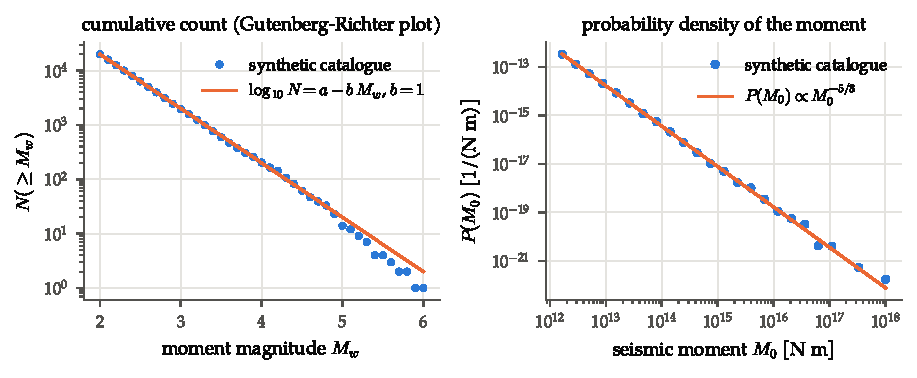
\includegraphics[width=\linewidth]{soc/gutenberg_richter.pdf}
  \caption{The two forms of the Gutenberg--Richter law, illustrated with a synthetic catalogue of
  $20\,000$ events generated with $b=1$ (not real data). Left: number of events with magnitude at
  least $M_w$, on a logarithmic vertical axis; the slope is $-b$. Right: the same events
  as a probability density of the seismic moment, on logarithmic axes; the slope is $-\tau=-5/3$.
  The scatter at the largest sizes is the statistical noise of the few largest events.}
  \label{fig:GR}
\end{figure}

\subsection{What the law means}

A probability density of the form $P(x)\propto x^{-\tau}$ is called a \emph{power law}, and $\tau$ is
its \emph{exponent}. Chapter~\ref{ch:soc} explains in detail why power laws are special. The main
point can be stated already: a power law has \emph{no characteristic scale}. There is no
``typical'' earthquake size, in the sense in which there is a typical height of a person; there
are simply fewer large events than small ones, in a fixed ratio for every factor of size.

A second consequence concerns which events dominate. The total moment released by all earthquakes
with moments between $M_{\min}$ and $M_{\max}$ is proportional to
\begin{equation}
  \int_{M_{\min}}^{M_{\max}} M_0\, P(M_0)\, \dd M_0 \;\propto\; \int_{M_{\min}}^{M_{\max}} M_0^{1-\tau}\,\dd M_0
  = \frac{M_{\max}^{2-\tau} - M_{\min}^{2-\tau}}{2-\tau} \;\approx\; \frac{M_{\max}^{1/3}}{1/3}
\end{equation}
for $\tau = 5/3$ and $M_{\max}\gg M_{\min}$. The result depends on the \emph{largest} events and hardly
at all on the smallest. Although small earthquakes are far more numerous, most of the slip on a fault
is accomplished by its few largest earthquakes.

\subsection{The magnitude used by Carlson and Langer}

The papers on the Burridge--Knopoff model that this thesis builds on~\cite{CarlsonLanger1989,Carlson1991}
use a different, simpler magnitude: the natural logarithm of the model's moment,
\begin{equation}
  \mu = \ln M .
\end{equation}
(Here $M$ is the moment of the model, defined in Chapter~4; $\mu$ is unrelated to the shear
modulus $\mu_{\mathrm s}$.) They write their results as a frequency density in $\mu$,
$\mathcal R(\mu)\propto e^{-b\mu}$, and call $b$ the $b$-value. To relate this to a power law in $M$,
note that the same events are counted whether we use $\mu$ or $M$:
$\mathcal R(\mu)\,\dd\mu = P(M)\,\dd M$. Since $\dd\mu = \dd M/M$,
\begin{equation}
  P(M) = \mathcal R(\mu)\frac{\dd\mu}{\dd M} = \frac{e^{-b\ln M}}{M} = M^{-(1+b)} .
  \label{eq:CL-b-tau}
\end{equation}
So in Carlson and Langer's language, ``$b=1$, consistent with Gutenberg--Richter'' means a moment density
$P(M)\propto M^{-2}$, i.e.\ $\tau = 2$, and \emph{not} the $\tau=5/3$ of \cref{eq:GR-density}. The two
$b$-values differ because the magnitudes are defined differently (natural logarithm and no factor
$2/3$). This difference must be kept in mind whenever results of the model are compared with
seismological data or with the exponents of sandpile models.

% ======================================================================
\section{Two kinds of models}
\label{sec:models}

Real faults are three-dimensional, heterogeneous, and only partly observable. To understand
\emph{why} the Gutenberg--Richter law holds, physicists have studied models that are deliberately
much simpler than a real fault but keep what is believed to be essential. Two families of models
are central to this thesis.

\subsection{The Burridge--Knopoff model}
\label{sec:bk-intro}

In 1967 Burridge and Knopoff~\cite{BurridgeKnopoff1967} proposed a mechanical model of a fault made of
blocks and springs (\cref{fig:bk-sketch}). A chain of $N$ identical blocks of mass $m$ rests on a rough,
fixed surface, which represents one side of the fault. Each block is connected
\begin{itemize}[nosep]
  \item to its two neighbours by \emph{coupling springs} of spring constant $k_c$, which represent the
    elastic stiffness of the rock along the fault;
  \item to a rigid upper plate by a \emph{pulling spring} of spring constant $k_p$, which represents the
    elastic connection of the fault zone to the far-away part of the moving plate.
\end{itemize}
The upper plate moves at a constant, very small velocity $v$. Between each block and the surface acts
a friction force with the stick--slip properties of \cref{sec:stickslip}: a block stays stuck until the
total spring force on it exceeds the maximum static friction $F_0$, and then slides with a kinetic
friction force that decreases with its velocity.

\begin{figure}[t]
\centering
\begin{tikzpicture}[x=10mm,y=10mm,>={Stealth[length=2mm]}]
  % floor
  \fill[pattern=north east lines,pattern color=ink2!60] (-0.4,-0.25) rectangle (10.4,0);
  \draw[ink2,thick] (-0.4,0) -- (10.4,0);
  \node[ink2,font=\footnotesize,anchor=west] at (10.5,-0.12) {fixed rough surface};
  % plate
  \fill[cblue!12] (-0.4,2.2) rectangle (10.4,2.6);
  \draw[ink2] (-0.4,2.2) rectangle (10.4,2.6);
  \node[font=\footnotesize,anchor=west] at (10.5,2.4) {plate, velocity $v$};
  \draw[->,cblueD,thick] (8.6,2.85) -- (10.0,2.85);
  % blocks
  \foreach \i in {0,...,4} {
    \pgfmathsetmacro\x{0.6+2.2*\i}
    \draw[ink2,fill=corange!20] (\x,0) rectangle (\x+1.0,0.8);
    \node[font=\footnotesize] at (\x+0.5,0.4) {$m$};
    % pulling spring
    \draw[ink2,decorate,decoration={zigzag,segment length=2.2mm,amplitude=1mm}] (\x+0.5,0.8) -- (\x+0.5,2.2);
  }
  \foreach \i in {0,...,3} {
    \pgfmathsetmacro\x{1.6+2.2*\i}
    \draw[ink2,decorate,decoration={zigzag,segment length=2.2mm,amplitude=1mm}] (\x,0.4) -- (\x+1.2,0.4);
  }
  \node[font=\footnotesize,ink2] at (2.2,0.75) {$k_c$};
  \node[font=\footnotesize,ink2,anchor=west] at (1.15,1.5) {$k_p$};
  \node[font=\footnotesize,ink2] at (5.5,-0.55) {friction $F(\dot x)$ between each block and the surface ($\dot x$: velocity of the block)};
\end{tikzpicture}
\caption{The Burridge--Knopoff model: blocks of mass $m$ connected to each other by coupling springs
$k_c$ and to a slowly moving plate by pulling springs $k_p$, sliding with stick--slip friction on a
fixed surface.}
\label{fig:bk-sketch}
\end{figure}

The dynamics is simple to state. The pulling springs are stretched slowly and uniformly by the plate.
When one block reaches the friction threshold, it slips; its motion changes the force on its neighbours
through the coupling springs, and they may slip too. The resulting cascade is a model earthquake. Its
size is measured by the moment, the sum of the displacements of all the blocks that moved, in close
analogy with \cref{eq:M0}.

Carlson and Langer~\cite{CarlsonLanger1989} studied this model in detail and found that, without any
randomness in the model, it produces a broad distribution of event sizes that is consistent with the
Gutenberg--Richter law for small and intermediate events, together with an excess of very large
events. The model and these results are the subject of Chapter~4.

\subsection{Sandpile models}

At almost the same time, Bak, Tang and Wiesenfeld~\cite{BTW1987,BTW1988} introduced a much simpler kind of
model, the \emph{sandpile model}. Grains are dropped one by one onto a lattice; when the number of grains
at a site exceeds a threshold, the site ``topples'' and passes grains to its neighbours, which may topple
in turn. The sandpile has no masses, velocities or forces, only integers and a rule. Yet it shows avalanches
of all sizes with power-law distributions, and it reaches this state by itself, without any parameter
being tuned. Bak, Tang and Wiesenfeld called this behaviour \emph{self-organized criticality} and proposed
that it explains the Gutenberg--Richter law, among many other power laws in nature. Chapter~\ref{ch:soc}
introduces these ideas in detail.

The analogy between the two kinds of models is clear: in both, a quantity (stress, grains) is loaded slowly,
released when a local threshold is exceeded, and redistributed to neighbours, producing avalanches. In 1992
Olami, Feder and Christensen~\cite{OFC1992} made the analogy precise for a two-dimensional version of the
Burridge--Knopoff model, by removing the inertia of the blocks and turning the model into a sandpile-like
automaton with continuous variables.

% ======================================================================
\section{This project}
\label{sec:project}

\subsection{The question}

The central question of this thesis is:
\begin{quote}
\emph{Can the statistics of the one-dimensional Burridge--Knopoff model be understood by mapping it onto a
sandpile model? If so, what are its critical exponents; if not, what exactly is lost in the mapping?}
\end{quote}
The mapping is attractive because sandpile models are far easier to simulate and, in some cases, to solve
exactly. But the Burridge--Knopoff model contains something that a sandpile does not: inertia. A slipping
block has kinetic energy, and Carlson and Langer showed that the largest events of the model are driven by
pulses of slip that grow as they propagate along the chain. It is therefore not obvious that a sandpile
can capture all of the model's behaviour.

\subsection{History of the project}

This thesis revives an earlier attempt at the same question. That attempt stalled at the first step: the
numerical simulations could not reproduce the size distributions published by Carlson and
Langer in 1989~\cite{CarlsonLanger1989}. Two reasons emerged. First, the 1989 paper was based on relatively
short simulations, and its later companion paper by Carlson, Langer, Shaw and Tang (1991)~\cite{Carlson1991}
uses a modified friction law and a different limit of the loading speed, with noticeably different results.
Second, a careful review of the old simulation code, carried out for this thesis, found several errors in
the numerical integration, in the boundary conditions and in the units of the parameters. The present work
therefore starts again from a clean, tested implementation.

\subsection{Aims}

The aims of this thesis are:
\begin{enumerate}[nosep]
  \item to review the theory of self-organized criticality and of sandpile models at the level needed for the
    project;
  \item to review the analysis of the Burridge--Knopoff model by Carlson and collaborators, and in particular
    to understand the differences between the 1989 and 1991 papers;
  \item to implement the Burridge--Knopoff model and the relevant sandpile models, and to verify the
    implementations against exactly known results;
  \item to reproduce the published results of the Burridge--Knopoff model;
  \item to derive the mapping from the Burridge--Knopoff model to a sandpile model, and to test by simulation
    where it holds and where it fails;
  \item to develop an approximate theory (of mean-field or branching-process type) for the exponents of the
    mapped model and to compare it with simulations.
\end{enumerate}

\subsection{Structure of the thesis}

Chapter~\ref{ch:soc} introduces power laws, critical phenomena and self-organized criticality, and studies the
Bak--Tang--Wiesenfeld sandpile in one and two dimensions, including an exact solution in one dimension.
Chapter~3 discusses how exponents are measured reliably from finite data. Chapter~4 presents the
Burridge--Knopoff model and the work of Carlson and collaborators. Chapter~5 derives the mapping to a sandpile
model. Chapter~6 describes the numerical methods and how they were validated, Chapter~7 presents the results,
Chapter~8 the approximate theory, and Chapter~9 summarises the conclusions.

\chapter{Self-organized criticality and sandpile models}
\label{ch:soc}

\newcommand{\socHeightSim}[1]{\ifcase#1 0.0738\or 0.1739\or 0.3057\or 0.4465\fi}
\newcommand{\socMeanHeightSim}{2.1249}
\newcommand{\socLmax}{512}
\newcommand{\socNav}{1{,}000{,}000}
\newcommand{\socDest}{2.81}
\newcommand{\socTauRel}{1.29}
\newcommand{\socMeanSim}{9299}
\newcommand{\socMeanExact}{9285}


This chapter develops the ideas needed to talk precisely about ``criticality'' in an
earthquake model. \Cref{sec:pl} defines probability distributions and power laws and
explains what makes power laws special. \Cref{sec:critical} recalls where power laws
appear in ordinary statistical physics, at critical points, using percolation as the
example. \Cref{sec:soc} presents the idea of self-organized criticality. The rest of the
chapter studies the Bak--Tang--Wiesenfeld (BTW) sandpile: its definition
(\cref{sec:btw-def}), its remarkable Abelian property (\cref{sec:abelian}), its long-time
behaviour (\cref{sec:stationary}), an exact formula for the mean avalanche size
(\cref{sec:mean}), a complete solution in one dimension (\cref{sec:btw1d}), and its
behaviour in two dimensions (\cref{sec:btw2d}). The chapter closes with what these results
imply for the Burridge--Knopoff model (\cref{sec:soc-implications}).

% ======================================================================
\section{Probability distributions and power laws}
\label{sec:pl}

\subsection{Basic definitions}

Throughout this thesis we deal with quantities that vary randomly from one event to the next:
the size of an avalanche, the moment of an earthquake. Let $x$ be such a quantity.

\begin{definition}
The \emph{probability density} $P(x)$ is defined so that $P(x)\,\dd x$ is the probability that
the quantity lies between $x$ and $x+\dd x$. It is non-negative and normalised,
$\int P(x)\,\dd x = 1$. If $x$ takes only integer values, as the number of topplings in an
avalanche does, $P(x)$ is the probability of the value $x$ and integrals become sums; we use the
same notation for both cases.
\end{definition}

\begin{definition}
The \emph{complementary cumulative distribution} is the probability that the quantity is at
least $x$,
\begin{equation}
  \bar F(x) = \int_x^\infty P(x')\,\dd x' , \qquad\text{so that}\qquad P(x) = -\frac{\dd \bar F}{\dd x}.
  \label{eq:Fbar}
\end{equation}
\end{definition}
The Gutenberg--Richter count $N(\geq M_w)$ of Chapter~\ref{ch:intro} is, up to the total number of
events, a complementary cumulative distribution.

\begin{definition}
The \emph{$q$-th moment} of the distribution is the average of $x^q$,
\begin{equation}
  \avg{x^q} = \int x^q P(x)\,\dd x .
\end{equation}
The first moment $\avg{x}$ is the mean.
\end{definition}

\subsection{Power laws}

\begin{definition}
A distribution is a \emph{power law} with \emph{exponent} $\tau$ if
\begin{equation}
  P(x) = C\, x^{-\tau}\qquad\text{for } x \ge x_{\min},
  \label{eq:pl}
\end{equation}
where $C$ is a normalisation constant and $x_{\min}>0$ is the smallest value considered.
\end{definition}

\paragraph{Why logarithmic axes.} Taking the logarithm of \cref{eq:pl} gives
\begin{equation}
  \log P = \log C - \tau \log x .
\end{equation}
In a plot of $\log P$ against $\log x$ (a ``log--log plot'') a power law is therefore a straight
line with slope $-\tau$. This is why distributions of avalanche and earthquake sizes are almost
always shown on logarithmic axes.

\paragraph{Normalisation.} The lower limit $x_{\min}$ is necessary: the integral of $x^{-\tau}$
diverges at $x\to0$ for every $\tau\ge1$. With $x_{\min}$ in place,
\begin{equation}
  \int_{x_{\min}}^{\infty} C x^{-\tau}\,\dd x
  = C \left[\frac{x^{1-\tau}}{1-\tau}\right]_{x_{\min}}^{\infty}
  = C\,\frac{x_{\min}^{1-\tau}}{\tau-1}\qquad(\tau>1).
\end{equation}
Setting this equal to 1 gives $C = (\tau-1)\,x_{\min}^{\tau-1}$. For $\tau\le1$ the integral diverges
at large $x$ and the distribution cannot be normalised without an upper limit as well.

\paragraph{Cumulative distribution.} Using \cref{eq:Fbar},
\begin{equation}
  \bar F(x) = \int_x^\infty (\tau-1)x_{\min}^{\tau-1}\, x'^{-\tau}\,\dd x'
  = \left(\frac{x}{x_{\min}}\right)^{-(\tau-1)} .
  \label{eq:Fbar-pl}
\end{equation}
The cumulative distribution of a power law is again a power law, with exponent smaller by one. This is
exactly the relation between the exponent $2b/3$ of the cumulative Gutenberg--Richter law and the
exponent $\tau = 1 + 2b/3$ of the density, found in \cref{eq:GR-density}.

\paragraph{The mean.} The mean of a pure power law is
\begin{equation}
  \avg{x} = \int_{x_{\min}}^{\infty} x\cdot C x^{-\tau}\,\dd x = C\left[\frac{x^{2-\tau}}{2-\tau}\right]_{x_{\min}}^{\infty}
  = \frac{\tau-1}{\tau-2}\,x_{\min}\qquad(\tau>2),
\end{equation}
and it is infinite for $\tau\le 2$. For the exponents met in this thesis ($1<\tau\le2$) the mean of a real,
finite system is therefore controlled by its \emph{largest} values. If the power law holds up to an upper
cutoff $x_c\gg x_{\min}$,
\begin{equation}
  \avg{x} \approx C\int_{x_{\min}}^{x_c} x^{1-\tau}\,\dd x = C\,\frac{x_c^{2-\tau} - x_{\min}^{2-\tau}}{2-\tau}
  \approx \frac{C}{2-\tau}\, x_c^{\,2-\tau}\qquad(1<\tau<2).
  \label{eq:mean-cutoff}
\end{equation}
The mean grows without bound as the cutoff grows. This simple formula will give an exact relation between
exponents in \cref{sec:mean}.

\subsection{Scale invariance}
\label{sec:scaleinv}

What makes power laws special is that they have \emph{no characteristic scale}. To see what this means,
compare a power law with an exponential distribution, $P(x)\propto e^{-x/\xi}$. The exponential contains a
scale $\xi$: values of $x$ much smaller than $\xi$ are common, values much larger than $\xi$ are
astronomically rare. If someone shows you a plot of the exponential over a window $[x_0, 10x_0]$, you can tell
from the shape where you are: for $x_0\ll\xi$ the curve is almost flat, for $x_0\gg\xi$ it drops like a cliff.

A power law looks the same in every window. Change the unit in which $x$ is measured by a factor $\lambda$:
\begin{equation}
  P(\lambda x) = C\,(\lambda x)^{-\tau} = \lambda^{-\tau}\,P(x).
  \label{eq:scaleinv}
\end{equation}
The rescaled function is the old function multiplied by a constant. On a plot where the vertical axis is
normalised to the value at the start of the window, all windows give the same curve
(\cref{fig:scaleinv}).

\begin{figure}[t]
  \centering
  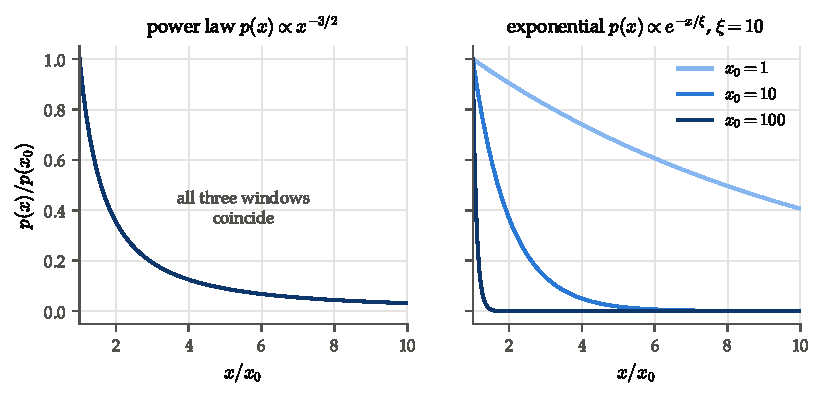
\includegraphics[width=\linewidth]{soc/scale_invariance.pdf}
  \caption{The same distribution seen through three windows $[x_0, 10x_0]$, with $x_0=1,10,100$. Each curve
  is divided by its value at the start of the window. Left: a power law gives the same curve in every window.
  Right: an exponential with scale $\xi=10$ looks completely different in each window.}
  \label{fig:scaleinv}
\end{figure}

Remarkably, the converse is also true: \emph{the power law is the only scale-invariant function}. Suppose
that rescaling $x$ by any factor $\lambda$ only multiplies $P$ by a factor $f(\lambda)$ that does not
depend on $x$:
\begin{equation}
  P(\lambda x) = f(\lambda)\,P(x)\qquad\text{for all } x,\lambda>0 .
  \label{eq:scaleinv-general}
\end{equation}
\begin{enumerate}
  \item Rescaling first by $\lambda_2$ and then by $\lambda_1$ is the same as rescaling once by
    $\lambda_1\lambda_2$. Applying \cref{eq:scaleinv-general} twice,
    $P(\lambda_1\lambda_2 x) = f(\lambda_1)f(\lambda_2)P(x)$; applying it once,
    $P(\lambda_1\lambda_2x) = f(\lambda_1\lambda_2)P(x)$. Hence
    \begin{equation}
      f(\lambda_1\lambda_2) = f(\lambda_1)\,f(\lambda_2).
    \end{equation}
  \item Differentiate with respect to $\lambda_1$ and then set $\lambda_1=1$:
    $\lambda_2 f'(\lambda_2) = f'(1)\,f(\lambda_2)$. Call the constant $f'(1) = -\tau$.
  \item The equation $\lambda f'(\lambda) = -\tau f(\lambda)$ is separable:
    $\dd f/f = -\tau\,\dd\lambda/\lambda$, so $\ln f = -\tau\ln\lambda + \text{const}$. Since $f(1)=1$,
    the constant is zero and $f(\lambda) = \lambda^{-\tau}$.
  \item Finally put $x=1$ in \cref{eq:scaleinv-general}: $P(\lambda) = \lambda^{-\tau}P(1)$. Renaming
    $\lambda\to x$, $P(x) = P(1)\,x^{-\tau}$, a power law.
\end{enumerate}

So when we observe a power law over many decades, we are observing a system in which nothing selects a
particular size. In physics, the classic situation where this happens is a critical point.

\paragraph{Cutoffs.} No real distribution is a power law for all $x$. There is always a smallest unit (one
grain, one block) and a largest possible event (set by the size of the system). A realistic form is
\begin{equation}
  P(x) = x^{-\tau}\,\mathcal{G}\!\left(\frac{x}{x_c}\right),
  \label{eq:cutoff-form}
\end{equation}
where the \emph{cutoff function} $\mathcal G(u)$ is approximately constant for $u\ll1$ and decays rapidly
for $u\gg1$, and $x_c$ is the \emph{cutoff}. The power law then holds in the window $x_{\min}\ll x\ll x_c$.
The important questions are what the exponent $\tau$ is in that window and how $x_c$ depends on the size of
the system.

% ======================================================================
\section{Power laws at critical points}
\label{sec:critical}

\subsection{Phase transitions}

A \emph{phase transition} is a qualitative change in the large-scale state of a system when a
\emph{control parameter} is varied: water boils when the temperature passes \SI{100}{\celsius} at
atmospheric pressure, and a piece of iron loses its magnetisation when heated above its Curie temperature,
about \SI{770}{\celsius}. The state on each side of the transition is characterised by an \emph{order
parameter}, a quantity that is zero in one phase and non-zero in the other, such as the magnetisation of the
iron.

Transitions come in two kinds. At a \emph{first-order} transition the order parameter jumps (liquid water
and steam have different densities at the boiling point). At a \emph{continuous} or \emph{critical}
transition it goes to zero continuously, and something remarkable happens: the system develops fluctuations
on all length scales at once. A fluid near its critical point becomes milky (``critical opalescence''),
because density fluctuations of all sizes, including sizes comparable to the wavelength of light, are present.

The quantity that makes this precise is the \emph{correlation length} $\xi$. It is the distance over which
the state of one part of the system influences the state of another part: two points much closer than $\xi$
behave in a correlated way, two points much farther apart than $\xi$ behave independently. Away from the
critical point $\xi$ is finite, a few molecular distances. At the critical point it diverges. Near the
critical point it diverges as a power of the distance from it, for example
\begin{equation}
  \xi \propto |T - T_c|^{-\nu},
\end{equation}
where $T_c$ is the critical temperature and $\nu$ is a \emph{critical exponent}. Other quantities have their
own exponents. A key discovery of the theory of critical phenomena is \emph{universality}: the critical
exponents do not depend on the details of a system, only on a few general properties such as the dimension
of space and the symmetries. The liquid--gas critical point of carbon dioxide and the critical point of a
certain class of magnets have the same exponents. This is why very simple models can predict exponents of
real systems exactly.

\subsection{Percolation: a geometric critical point}

The simplest model with a critical point is \emph{percolation}~\cite{Stauffer1994}. Each site of a lattice
is occupied with probability $p$ and empty with probability $1-p$, independently of all other sites.
Neighbouring occupied sites form \emph{clusters} (\cref{fig:percolation}). The control parameter is $p$.

\begin{figure}[t]
  \centering
  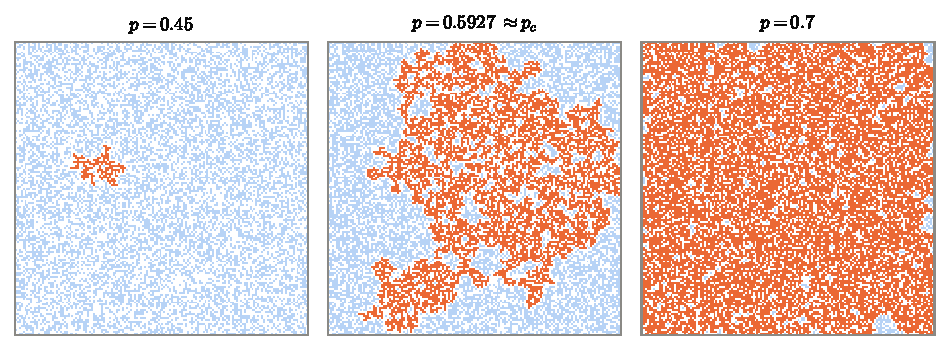
\includegraphics[width=\linewidth]{soc/percolation.pdf}
  \caption{Site percolation on a $150\times150$ square lattice. Occupied sites are light blue, and the largest
  cluster is orange. Below the threshold (left) the largest cluster is small. At the threshold
  $p_c\approx0.5927$ (middle) it is a ragged, fractal object with holes of all sizes. Above it (right) it fills
  most of the lattice.}
  \label{fig:percolation}
\end{figure}

For small $p$ the clusters are small and isolated. For $p$ close to 1 almost everything is connected into one
huge cluster. In between, at a sharp \emph{percolation threshold} $p_c$ ($p_c\approx 0.5927$ for sites of the
square lattice), an infinite cluster appears for the first time. The order parameter is the probability that a
site belongs to the infinite cluster. The correlation length is the typical radius of the finite clusters, and
it diverges at the threshold, $\xi\propto|p-p_c|^{-\nu}$ with $\nu = 4/3$ in two dimensions.

The cluster sizes are described by the \emph{cluster number} $n_s$, the number of clusters containing exactly
$s$ sites, divided by the number of lattice sites. Near $p_c$ it has the form
\begin{equation}
  n_s \simeq s^{-\tau}\,\mathcal G\!\left(\frac{s}{s_\xi}\right),\qquad s_\xi \propto \xi^{D},
  \label{eq:perc-scaling}
\end{equation}
which is exactly the cutoff form \cref{eq:cutoff-form}. In two dimensions $\tau = 187/91\approx2.06$. The
cutoff $s_\xi$ is the size of a cluster whose radius is $\xi$, and $D=91/48\approx1.90$ is the \emph{fractal
dimension} of the clusters: a cluster of radius $R$ contains about $R^{D}$ sites, fewer than the $R^2$ sites of
a filled disc, because it is full of holes (\cref{fig:percolation}, middle). Only exactly at $p=p_c$, where
$s_\xi=\infty$, is the cluster distribution a pure power law.

\subsection{One-dimensional percolation, worked out}
\label{sec:perc1d}

In one dimension percolation can be solved with elementary probability, and the solution is instructive
because the same features will appear in the one-dimensional sandpile.

\paragraph{Cluster numbers.} On a chain, a cluster of exactly $s$ sites that starts at a given site $i$ requires
sites $i,\dots,i+s-1$ to be occupied (probability $p^s$) and the two sites just outside, $i-1$ and $i+s$, to be
empty (probability $(1-p)^2$). Hence
\begin{equation}
  n_s = (1-p)^2\, p^{s} = (1-p)^2\, e^{-s/s_\xi},\qquad s_\xi = -\frac{1}{\ln p} .
\end{equation}
This is an \emph{exponential}, not a power law: for every $p<1$ there is a characteristic cluster size $s_\xi$.

\paragraph{Mean cluster size.} Pick an occupied site at random and ask for the size of its cluster. A cluster of
size $s$ contains $s$ sites, so the probability that the chosen site belongs to a cluster of size $s$ is
proportional to $s\,n_s$. The mean cluster size is therefore $S = \sum_s s^2 n_s / \sum_s s\,n_s$. Using the sums
$\sum_{s\ge1} s\,p^s = p/(1-p)^2$ and $\sum_{s\ge1}s^2p^s = p(1+p)/(1-p)^3$,
\begin{equation}
  \sum_s s\, n_s = (1-p)^2\frac{p}{(1-p)^2} = p, \qquad
  \sum_s s^2 n_s = (1-p)^2\frac{p(1+p)}{(1-p)^3} = \frac{p(1+p)}{1-p},
\end{equation}
\begin{equation}
  S = \frac{1+p}{1-p} .
\end{equation}
(The first sum is a check: it is the fraction of occupied sites, $p$.) The mean cluster size diverges as
$(1-p)^{-1}$ when $p\to1$, a power law with exponent $\gamma=1$.

\paragraph{Correlation length.} Two sites at distance $r$ belong to the same cluster only if all $r+1$ sites from
one to the other are occupied. Given that the first is occupied, this has probability $p^{r} = e^{-r/\xi}$ with
$\xi = -1/\ln p$. As $p\to1$, $\ln p\approx -(1-p)$ and $\xi\approx(1-p)^{-1}$, so $\nu = 1$.

\paragraph{Lesson.} The critical point of one-dimensional percolation is at $p_c = 1$, the very edge of the range
of $p$. There the ``critical state'' is the trivial fully occupied chain, with a single cluster. A single empty
site cuts a chain, so in one dimension it is very hard to build long-range connections. One-dimensional
systems are special in this way, and we will meet the same situation in the sandpile.

\subsection{The problem of fine tuning}

In all these examples a power law appears only at one special value of the control parameter ($T_c$, $p_c$).
An experimentalist who wants to observe it must tune the parameter to that value with great precision. But
earthquakes obey the Gutenberg--Richter law everywhere, and nobody tunes the Earth's crust. This puzzle is
the starting point of self-organized criticality.

% ======================================================================
\section{Self-organized criticality}
\label{sec:soc}

\subsection{The idea}

In 1987 Bak, Tang and Wiesenfeld~\cite{BTW1987,BTW1988} proposed that some systems are driven \emph{to} a
critical point by their own dynamics. They called this \emph{self-organized criticality} (SOC). In the
self-organized critical state a small perturbation can trigger a response, an \emph{avalanche}, of any size, and
the sizes follow a power law, without any parameter having been tuned. The systems they had in mind share four
ingredients~\cite{Jensen1998,Charbonneau2017}:
\begin{enumerate}
  \item \textbf{Slow driving.} Some quantity (sand, stress, energy) is added to the system slowly, a little at a
    time.
  \item \textbf{A local threshold.} Nothing happens at a point of the system until a local variable exceeds a
    critical value. Below the threshold the system is stable; it can store the added quantity.
  \item \textbf{Fast local relaxation.} When the threshold is exceeded at a point, the quantity stored there is
    passed to the neighbouring points. They may exceed their own threshold and pass it on, and so on: this
    chain reaction is the avalanche.
  \item \textbf{Dissipation.} The quantity must be able to leave the system, for example through its boundary;
    otherwise it would accumulate forever and no steady state could exist.
\end{enumerate}
The driving must be slow compared with the relaxation: an avalanche must be finished before the next unit is
added, so that avalanches are distinct events. This is the \emph{separation of time scales}.

\Cref{tab:soc-analogy} shows how these ingredients appear in a sandpile and in an earthquake fault. The
separation of time scales on a real fault, estimated in \cref{sec:stickslip}, is about $10^{-8}$.

\begin{table}[t]
\centering
\caption{The ingredients of self-organized criticality in a sandpile and in an earthquake fault.}
\label{tab:soc-analogy}
\begin{tabular}{@{}p{22mm}p{50mm}p{70mm}@{}}
\toprule
ingredient & sandpile & earthquake fault (BK model) \\
\midrule
slow drive & grains added one at a time & plate moves at velocity $v$ \\
threshold & critical height $z_c$ & maximum static friction $F_0$ \\
relaxation & toppling to neighbours & slip; force passed through coupling springs $k_c$ \\
dissipation & grains leave at the boundary & energy lost to friction; stress taken up by pulling springs $k_p$ \\
\bottomrule
\end{tabular}
\end{table}

\subsection{Why the critical point is an attractor}

The reason a system can organise itself to a critical point can be understood with a feedback argument.
Think of a sandpile with some average density of grains $\zeta$. If the density is low, an added grain causes
only a small avalanche, which does not reach the boundary: grains accumulate and $\zeta$ increases. If the
density is high, added grains cause huge avalanches that carry many grains out through the boundary: $\zeta$
decreases. The density is pushed towards the special value $\zeta_c$ between the two regimes, where avalanches
are just barely able to propagate to any distance. That value is a critical point, and the slow drive and the
boundary dissipation together hold the system there.

This argument also shows the limits of the idea. The critical density is reached only if the drive is slow
enough (otherwise avalanches overlap and the system is pushed above $\zeta_c$) and if grains are lost only at the
boundary (if grains are lost inside the system, avalanches die out before they reach a large size, and the
system settles below $\zeta_c$). In a precise sense, then, ``self-organized'' criticality still needs two
parameters to be at a limiting value: the driving rate and the bulk dissipation must both go to zero. This view,
that SOC is an ordinary critical point whose control parameter is tuned automatically by a feedback, was made
precise by Dickman, Vespignani and Zapperi~\cite{DickmanVespignaniZapperi1998}. It is directly relevant to
earthquake models, in which the pulling springs remove stress inside the system: we will see in Chapter~4 that
Carlson and collaborators found the size of the largest ``critical'' events of the Burridge--Knopoff model to be
controlled by exactly such parameters.

% ======================================================================
\section{The Bak--Tang--Wiesenfeld sandpile}
\label{sec:btw-def}

\subsection{Definition}

The BTW sandpile is defined on a lattice: a chain of $L$ sites in one dimension, or a square grid of $L\times L$
sites in two dimensions. The sites are numbered $i=1,\dots,N$, with $N=L$ or $N = L^2$. Each site has a set of
\emph{neighbours}: on the chain, the sites to its left and right; on the square lattice, the four sites above,
below, left and right. The number of neighbours of a site in the interior is called $k$ ($k=2$ in one dimension,
$k=4$ in two). Sites on the edge of the lattice have fewer neighbours inside the lattice; we say that their
missing neighbours are ``outside''.

The state of the system is described by integers $z_i\ge0$, called \emph{heights}, which we picture as the
number of grains of sand at each site. The dynamics has two parts.
\begin{enumerate}
  \item \textbf{Driving.} Choose a site $j$ at random, each site with equal probability $1/N$, and add one grain:
    $z_j\to z_j+1$.
  \item \textbf{Toppling.} A site is \emph{stable} if $z_i < z_c$ and \emph{unstable} if $z_i\ge z_c$, where
    $z_c = k$ is the \emph{critical height}. An unstable site \emph{topples}: it loses $k$ grains, and each of its
    $k$ neighbours gains one grain,
    \begin{equation}
      z_i \to z_i - k,\qquad z_{m} \to z_{m}+1 \ \text{ for every neighbour } m \text{ of } i.
    \end{equation}
    If $i$ is on the edge, the grains sent to its missing neighbours fall off the lattice and are lost.
\end{enumerate}
After a grain is added, topplings continue until all sites are stable again. The sequence of topplings caused by
one added grain is an \emph{avalanche}. Only when the avalanche is over is the next grain added: this is the
separation of time scales of \cref{sec:soc}, built into the rules. Grains are conserved in every toppling except
those of edge sites, so the edges play the role of dissipation. A lattice whose edges lose grains in this way is
said to have \emph{open boundaries}.

The possible heights of a stable site are $0,1,\dots,k-1$: $0$ or $1$ on the chain, and $0,1,2,3$ on the square
lattice. The toppling rule is illustrated in \cref{fig:toppling}.

\begin{figure}[t]
\centering
\begin{tikzpicture}[x=9mm,y=9mm,>={Stealth[length=1.6mm]}]
  \foreach \i/\h in {1/1,2/1,3/2,4/0,5/1} {
    \draw[ink2,fill=\ifnum\h>1 corange!25\else cblue!10\fi] (\i-0.4,0) rectangle (\i+0.4,0.7);
    \node[font=\small] at (\i,0.35) {\h};
  }
  \node[font=\small,ink2] at (-0.1,0.35) {outside};
  \node[font=\small,ink2] at (6.1,0.35) {outside};
  \draw[->,corange,thick] (3,0.85) to[bend right=40] (2,0.85);
  \draw[->,corange,thick] (3,0.85) to[bend left=40] (4,0.85);
  \node[font=\footnotesize,ink2,align=center] at (3,-0.6) {chain, $k=2$: site 3 is unstable;\\it loses 2 grains, sites 2 and 4 gain 1 each};
  \begin{scope}[xshift=72mm,yshift=-4mm]
  \foreach \x in {0,1,2} \foreach \y in {0,1,2} {
    \pgfmathtruncatemacro\c{(\x==1 && \y==1)}
    \ifnum\c=1 \def\fillc{corange!25}\else\def\fillc{cblue!10}\fi
    \draw[ink2,fill=\fillc] (\x-0.4,\y-0.4) rectangle (\x+0.4,\y+0.4);
  }
  \node[font=\small] at (1,1) {4};
  \foreach \dx/\dy in {1/0,-1/0,0/1,0/-1} \draw[->,corange,thick] (1+0.25*\dx,1+0.25*\dy) -- (1+0.75*\dx,1+0.75*\dy);
  \node[font=\footnotesize,ink2,align=center] at (1,-1.1) {square lattice, $k=4$:\\one grain to each neighbour};
  \end{scope}
\end{tikzpicture}
\caption{The toppling rule of the BTW sandpile.}
\label{fig:toppling}
\end{figure}

\subsection{Measuring an avalanche}

For each added grain we record four numbers:
\begin{itemize}[nosep]
  \item the \textbf{size} $s$: the total number of topplings;
  \item the \textbf{area} $a$: the number of different sites that toppled at least once;
  \item the \textbf{duration} $T$: the number of time steps, where in each time step all the sites that are
    unstable at the beginning of the step topple once, simultaneously (the \emph{parallel update});
  \item the number of grains \textbf{lost} through the boundary.
\end{itemize}

\begin{example}
\label{ex:avalanche}
Take a chain of $L=5$ sites with heights $(1,1,1,1,0)$ and add a grain at site $j=2$. The avalanche proceeds as
follows (unstable sites in bold):
\begin{center}
\begin{tabular}{clc}
\toprule
step & heights & sites that topple \\
\midrule
start & $(1,\mathbf{2},1,1,0)$ & 2 \\
1 & $(\mathbf{2},0,\mathbf{2},1,0)$ & 1, 3 \\
2 & $(0,\mathbf{2},0,\mathbf{2},0)$ & 2, 4 \\
3 & $(1,0,\mathbf{2},0,1)$ & 3 \\
4 & $(1,1,0,1,1)$ & --- \\
\bottomrule
\end{tabular}
\end{center}
In step 1, site 2 toppled and gave one grain each to sites 1 and 3. In step 2, sites 1 and 3 toppled together;
site 1 sent one of its two grains outside, where it was lost. The avalanche has size $s = 1+2+2+1 = 6$, area $a=4$
(sites 1--4 toppled), duration $T=4$, and one grain was lost. Grain count: $4$ grains at the start, plus one added,
minus one lost, equals the $4$ grains at the end.
\end{example}

\subsection{The toppling matrix}

It is convenient to write the toppling rule with a matrix. The \emph{toppling matrix} $\Delta$ is the $N\times N$
matrix with
\begin{equation}
  \Delta_{ii} = k, \qquad \Delta_{im} = -1 \text{ if $i$ and $m$ are neighbours},\qquad \Delta_{im}=0 \text{ otherwise}.
\end{equation}
Toppling site $i$ changes the heights by $z_m \to z_m - \Delta_{im}$ for every $m$: site $i$ loses $k$, each
neighbour gains $1$. For example, for a chain of $L=3$ sites,
\begin{equation}
  \Delta = \begin{pmatrix} 2 & -1 & 0\\ -1 & 2 & -1 \\ 0 & -1 & 2 \end{pmatrix}.
  \label{eq:Delta3}
\end{equation}
Row 1 shows that toppling site 1 removes two grains from it and gives one to site 2; the second grain goes outside
and does not appear in the matrix.

Now suppose a grain is added at site $j$ and, during the avalanche, each site $i$ topples $n_i$ times. Every toppling
of $i$ subtracts row $i$ of $\Delta$ from the configuration, so the heights after the avalanche are
\begin{equation}
  z^{\text{after}} = z^{\text{before}} + e_j - \Delta\, n ,
  \label{eq:balance}
\end{equation}
where $e_j$ is the vector with a 1 at position $j$ and zeros elsewhere, and $n=(n_1,\dots,n_N)$ is the vector of
toppling numbers. (We used that $\Delta$ is symmetric.) This \emph{balance equation} is the basis of all the exact
results below. Up to the sign, $\Delta$ is the discrete Laplacian, the lattice version of $\nabla^2$, with the
condition that the function vanishes outside the lattice. Because the edges lose grains, $\Delta$ is invertible; its
inverse
\begin{equation}
  G = \Delta^{-1}
\end{equation}
is called the \emph{Green function} of the lattice. For the chain of \cref{eq:Delta3} one finds
\begin{equation}
  G = \frac14\begin{pmatrix} 3 & 2 & 1\\ 2 & 4 & 2 \\ 1 & 2 & 3 \end{pmatrix},
  \label{eq:G3}
\end{equation}
as can be checked by multiplying with $\Delta$.

% ======================================================================
\section{The Abelian property}
\label{sec:abelian}

During an avalanche several sites can be unstable at the same time. Does it matter which one topples first? For the
BTW sandpile the remarkable answer, found by Dhar~\cite{Dhar1990}, is no.

\begin{example}
Take a chain of $L=3$ sites with heights $(2,0,2)$: sites 1 and 3 are unstable.
\begin{center}
\begin{tabular}{ll@{\qquad}ll}
\toprule
\multicolumn{2}{c}{site 1 first} & \multicolumn{2}{c}{site 3 first} \\
\midrule
topple 1: & $(0,1,2)$ & topple 3: & $(2,1,0)$ \\
topple 3: & $(0,2,0)$ & topple 1: & $(0,2,0)$ \\
topple 2: & $(1,0,1)$ & topple 2: & $(1,0,1)$ \\
\bottomrule
\end{tabular}
\end{center}
Both orders give the same final configuration $(1,0,1)$, with the same three topplings, one at each site.
\end{example}

The reason is simple. Toppling a site only \emph{adds} grains to other sites, so it can never make another unstable
site stable; and the effect of a toppling is to subtract a fixed vector, a row of $\Delta$, and subtractions can be
done in any order. Dhar turned this into a theorem.

\begin{theorem}[Abelian property~\cite{Dhar1990}]
\label{thm:abelian}
Whatever order is used to topple unstable sites, an avalanche ends in the same stable configuration, and every site
topples the same number of times. Consequently the size $s$ and the area $a$ of an avalanche do not depend on the order.
\end{theorem}

\begin{proof}
Let $\alpha$ and $\beta$ be two ways of toppling (each toppling being of a site that is unstable at that moment), both
continued until every site is stable. Let $n^\alpha_x$ be the number of times site $x$ topples in $\alpha$.

We show first that $\beta$ never topples a site more often than $\alpha$ does. Suppose this were false, and look at the
first moment in $\beta$ at which some site $x$ is about to topple for the $(n^\alpha_x+1)$-th time. Up to that moment
every other site has toppled in $\beta$ at most as often as in all of $\alpha$. Compare two configurations: the one
just before this toppling in $\beta$, and the final configuration of $\alpha$. In both, site $x$ has toppled
$n^\alpha_x$ times, so it has lost the same number of grains. But in $\alpha$ each neighbour of $x$ has toppled at least
as often as in $\beta$ so far, so in $\alpha$ site $x$ has \emph{received} at least as many grains. Hence the height of
$x$ at the end of $\alpha$ is at least its height now in $\beta$, which is $\ge z_c$ because $x$ is about to topple. That
contradicts the fact that $\alpha$ ends with all sites stable.

Exchanging the roles of $\alpha$ and $\beta$ shows that $\alpha$ never topples a site more often than $\beta$. So both
topple every site the same number of times: they have the same vector $n$, and by \cref{eq:balance} they end in the
same configuration. The size $s = \sum_x n_x$ and the area (the number of $x$ with $n_x>0$) are therefore the same.
\end{proof}

Two consequences are worth stating. First, if we call $A_j$ the operation ``add a grain at $j$ and relax'', then
$A_jA_m = A_mA_j$: adding two grains gives the same result in either order. Operations that commute are called
\emph{Abelian} in mathematics, hence the name \emph{Abelian sandpile model}. Second, the theorem says nothing about the
duration $T$, which does depend on the order of topplings; that is why the parallel update is fixed in its definition.

% ======================================================================
\section{The long-time behaviour}
\label{sec:stationary}

\subsection{Transient and recurrent configurations}

If we keep adding grains, the sandpile wanders through its stable configurations. Its future depends only on the
present configuration and on the random choice of the next site, so the sequence of configurations is a
\emph{Markov chain}. Some configurations are visited only at the beginning and never again; they are called
\emph{transient}. The others are visited again and again for ever; they are called \emph{recurrent}. After a long
time the system is found only in recurrent configurations, and the fraction of time it spends in each of them
settles down to a fixed value. This long-time situation is the \emph{stationary state}, and all the statistics in
this thesis are measured in it.

\begin{example}
\label{ex:L2}
For a chain of $L=2$ sites there are four stable configurations: $(0,0)$, $(0,1)$, $(1,0)$ and $(1,1)$. Working out
all possible additions gives the transitions
\begin{center}
\begin{tabular}{lll}
\toprule
from & grain at site 1 & grain at site 2 \\
\midrule
$(0,0)$ & $(1,0)$ & $(0,1)$ \\
$(0,1)$ & $(1,1)$ & $(1,0)$ \\
$(1,0)$ & $(0,1)$ & $(1,1)$ \\
$(1,1)$ & $(1,0)$ & $(0,1)$ \\
\bottomrule
\end{tabular}
\end{center}
For instance, from $(1,1)$ a grain at site 1 gives $(2,1)$; site 1 topples to $(0,2)$, losing a grain; then site 2
topples to $(1,0)$, losing another. The configuration $(0,0)$ does not appear in the last two columns: once the system
has left it, it never returns. So $(0,0)$ is transient and the other three are recurrent. Each of the three is
reached from the other two with equal probability, so in the stationary state each is found $1/3$ of the time.
\end{example}

\subsection{Dhar's results}

For the BTW model on any lattice, Dhar proved the following general results~\cite{Dhar1990,Dhar2006}:
\begin{enumerate}
  \item In the stationary state \textbf{all recurrent configurations are equally likely}.
  \item The \textbf{number of recurrent configurations} equals $\det\Delta$. (For $L=2$,
    $\det\begin{pmatrix}2&-1\\-1&2\end{pmatrix} = 3$, in agreement with \cref{ex:L2}.)
  \item A stable configuration is recurrent if and only if it contains no \textbf{forbidden subconfiguration}: a
    group $F$ of sites such that every site of $F$ has a height smaller than the number of its neighbours that
    belong to $F$. In \cref{ex:L2}, $(0,0)$ is forbidden with $F=\{1,2\}$: each site has height 0 but one neighbour in $F$.
\end{enumerate}
The intuition behind the last point is that a toppling always leaves grains on the neighbours of the toppled site, so
a group of sites that are all ``too empty'' relative to each other cannot be produced by topplings. In practice
these results tell us how to start a simulation: the configuration with every $z_i=k-1$ is always recurrent, so we
start from it and let the system run long enough to forget the starting point.

% ======================================================================
\section{An exact formula for the mean avalanche size}
\label{sec:mean}

The Abelian structure makes it possible to compute the mean avalanche size exactly, on any lattice and in any
dimension. Let $n_{ij}$ be the number of times site $i$ topples when a grain is added at site $j$. It depends on the
configuration at the moment the grain is added, so it is a random quantity. Its average over the stationary state can
be found in three steps.

\begin{enumerate}
  \item Write the balance equation \cref{eq:balance} for a grain added at $j$, component by component:
    $z_i^{\text{after}} = z_i^{\text{before}} + \delta_{ij} - \sum_m \Delta_{im} n_{mj}$.
  \item Average over the stationary state. In the stationary state the average height of each site does not change
    when a grain is added, $\avg{z_i^{\text{after}}} = \avg{z_i^{\text{before}}}$. (This needs one small observation:
    because all recurrent configurations are equally likely and $A_j$ maps recurrent configurations one-to-one onto
    recurrent configurations, the configuration after the addition is again distributed according to the stationary
    state.) Therefore
    \begin{equation}
      0 = \delta_{ij} - \sum_m \Delta_{im}\avg{n_{mj}} .
    \end{equation}
  \item In matrix form this reads $\Delta\avg{n} = I$, where $I$ is the identity matrix, so
    \begin{equation}
      \boxed{\;\avg{n_{ij}} = G_{ij},\qquad G=\Delta^{-1}.\;}
      \label{eq:nG}
    \end{equation}
\end{enumerate}
The average number of topplings at $i$ caused by a grain at $j$ is just the Green function. Summing over $i$, the mean
size of an avalanche started at $j$ is $g_j = \sum_i G_{ij}$, and for random (uniform) seeding
\begin{equation}
  \avg{s} = \frac1N\sum_{j} g_j = \frac1N\sum_{i,j} G_{ij}.
  \label{eq:mean-s}
\end{equation}

\begin{example}
For the chain of three sites, \cref{eq:G3} gives $g_1 = \tfrac14(3+2+1)=\tfrac32$, $g_2 = \tfrac14(2+4+2)=2$,
$g_3=\tfrac32$, and $\avg{s} = \tfrac13(\tfrac32+2+\tfrac32)=\tfrac53$. We will confirm this by listing every avalanche
in \cref{sec:btw1d}.
\end{example}

\paragraph{Intuition: a random walk.} Why should a Green function appear? Follow one particular grain through an
avalanche. Every time the site holding it topples, the grain is sent to a neighbour; since all grains at a site are
alike, we may take that neighbour to be chosen at random. So the grain performs a \emph{random walk} on the lattice
until it falls off the edge. The Green function of the Laplacian is exactly the quantity that counts how often such a
walk visits each site: $k\,G_{ij}$ is the average number of visits to site $i$ of a random walk that starts at $j$ and
stops when it leaves the lattice. In the stationary state, adding one grain causes on average as many topplings as the
walk of that grain makes steps.

\paragraph{How $\avg{s}$ grows with the system size.} A random walk moves a distance of order $\sqrt{t}$ in $t$ steps,
so to travel the distance $L$ to the boundary it needs about $L^2$ steps. Therefore
\begin{equation}
  \avg{s}\propto L^{2}\qquad\text{in every dimension}.
  \label{eq:mean-L2}
\end{equation}
The constant can be found from the continuum limit. For large $L$, $\Delta$ acts on smooth functions as $-\nabla^2$, so
$g$ solves the Poisson equation $-\nabla^2 g = 1$ inside the system with $g = 0$ on the boundary. Writing $g = L^2 w(x)$
with $x = j/L$ the position measured in units of $L$, the function $w$ solves $-\nabla^2 w = 1$ on the unit interval or
unit square, and $\avg{s}\simeq L^2\int w$. In one dimension $-w'' = 1$ with $w(0)=w(1)=0$ gives $w = x(1-x)/2$ and
$\int_0^1 w\,\dd x = 1/12$, so $\avg{s}\simeq L^2/12$. In two dimensions the same calculation with a Fourier series gives
$\int w \approx 0.0351$, so $\avg{s}\simeq0.0351\,L^2$.

\paragraph{A relation between exponents.} Suppose the avalanche sizes follow the cutoff form \cref{eq:cutoff-form},
\begin{equation}
  P(s) = s^{-\tau}\,\mathcal G\!\left(\frac{s}{s_c}\right),\qquad s_c\propto L^{D},
  \label{eq:fss}
\end{equation}
with $1<\tau<2$: the cutoff $s_c$ is set by the system size, and $D$ says how fast it grows. By \cref{eq:mean-cutoff},
$\avg{s}\propto s_c^{2-\tau}\propto L^{D(2-\tau)}$. Comparing with \cref{eq:mean-L2},
\begin{equation}
  \boxed{\;D\,(2-\tau) = 2.\;}
  \label{eq:scaling-relation}
\end{equation}
Of the two exponents $\tau$ and $D$, only one is independent. This exact relation is a direct consequence of grain
conservation in the bulk; we will see in \cref{sec:soc-implications} why it does not carry over to the
Burridge--Knopoff model.

% ======================================================================
\section{The one-dimensional sandpile: an exact solution}
\label{sec:btw1d}

On a chain ($k=2$, $z_c=2$, heights $0$ or $1$) the BTW model can be solved completely. We first find the recurrent
configurations, then compute what a single added grain does, and finally obtain the distribution of avalanche sizes.

\subsection{The recurrent configurations}

\paragraph{At most one empty site.} Suppose a configuration has two empty sites (height 0), and take two that have no
other empty site between them. Let $F$ be the set of sites from the first to the second. The two end sites of $F$ have
height 0 and one neighbour in $F$; the sites in between have height 1 and two neighbours in $F$. Every site of $F$ has a
height smaller than its number of neighbours in $F$, so $F$ is forbidden and the configuration is transient. Therefore a
recurrent configuration has \emph{at most one} empty site.

\paragraph{All of them are recurrent.} There are $L+1$ such configurations: the one with no empty site, and the $L$ with a
single empty site. To show that all of them are recurrent we use Dhar's result $|\mathcal R| = \det\Delta$. Call $d_L$ the
determinant of the $L\times L$ matrix $\Delta$. Expanding along the first row,
\begin{equation}
  d_L = 2\,d_{L-1} - d_{L-2},
\end{equation}
with $d_1 = 2$ and $d_2 = 3$. Then $d_3 = 2\cdot3-2 = 4$, $d_4 = 2\cdot4-3 = 5$, and in general $d_L = L+1$. So there are
exactly $L+1$ recurrent configurations, and these are all the configurations with at most one empty site. In the
stationary state each of them has probability $1/(L+1)$.

We label them by the position $l$ of the empty site, $l = 1,\dots,L$, and use $l=0$ for the configuration with no empty
site. For $L=3$:
\[
  l=0:\ (1,1,1),\qquad l=1:\ (0,1,1),\qquad l=2:\ (1,0,1),\qquad l=3:\ (1,1,0).
\]

\subsection{The Green function of the chain}

To use \cref{eq:balance} we need $G=\Delta^{-1}$ for the chain. Fix $j$ and look for the column $G_{ij}$ as a function of $i$.
It must satisfy $(\Delta G)_{ij} = \delta_{ij}$, that is,
\begin{equation}
  2G_{ij} - G_{i-1,j} - G_{i+1,j} = \delta_{ij},\qquad i=1,\dots,L,
  \label{eq:G-eq}
\end{equation}
with $G_{0j} = G_{L+1,j} = 0$ (there are no grains outside the chain).
\begin{enumerate}
  \item For $i\neq j$ the right-hand side is zero, so $G_{i+1,j}-G_{ij} = G_{ij}-G_{i-1,j}$: the differences are constant
    and $G_{ij}$ is a \emph{straight line} in $i$ on each side of $j$.
  \item The boundary conditions fix the lines to pass through zero at the two ends:
    $G_{ij} = A\,i$ for $i\le j$ and $G_{ij} = B\,(L+1-i)$ for $i\ge j$.
  \item The two lines must meet at $i=j$: $A j = B(L+1-j)$.
  \item At $i=j$ the equation has right-hand side 1. Inserting $G_{jj}=Aj$, $G_{j-1,j}=A(j-1)$ and
    $G_{j+1,j}=B(L-j)$ gives
    \[
      2Aj - A(j-1) - B(L-j) = Aj + A - B(L-j) = 1 .
    \]
    Replacing $Aj$ by $B(L+1-j)$ (step 3), the left-hand side becomes $B(L+1-j) + A - B(L-j) = A + B$, so $A+B = 1$.
  \item Solving $A+B=1$ together with $Aj = B(L+1-j)$ gives $B = j/(L+1)$ and $A = (L+1-j)/(L+1)$. For $i\le j$,
    $G_{ij} = Ai = i - ij/(L+1)$; for $i\ge j$, $G_{ij} = B(L+1-i) = j - ij/(L+1)$.
\end{enumerate}
Both cases combine into one formula:
\begin{equation}
  G_{ij} = \min(i,j) - \frac{i\,j}{L+1}.
  \label{eq:G1d}
\end{equation}
For $L=3$ this reproduces \cref{eq:G3}; for example $G_{11} = 1 - \tfrac14 = \tfrac34$ and $G_{22} = 2-1 = 1$. Summing over $i$,
\begin{equation}
  g(j) \equiv \sum_{i=1}^{L} G_{ij} = \frac{j\,(L+1-j)}{2},
  \label{eq:g1d}
\end{equation}
which is the mean avalanche size for a grain added at $j$. It is largest in the middle of the chain.

\subsection{All avalanches of the three-site chain}

Before treating general $L$, it is useful to look at every possible avalanche for $L=3$. There are four recurrent
configurations and three sites at which the grain can be added, so twelve cases, all equally likely.
Working each of them out by hand, as in \cref{ex:avalanche}, gives \cref{tab:L3}.

\begin{table}[t]
\centering
\caption{All twelve avalanches of the three-site chain in the stationary state: the initial configuration (labelled by the
position $l$ of its empty site), the site $j$ where the grain is added, the avalanche size $s$, and the label $l'$ of the
final configuration.}
\label{tab:L3}
\begin{tabular}{cc@{\qquad}ccc@{\qquad}ccc@{\qquad}ccc}
\toprule
& & \multicolumn{2}{c}{$j=1$} & & \multicolumn{2}{c}{$j=2$} & & \multicolumn{2}{c}{$j=3$} \\
$l$ & configuration & $s$ & $l'$ & & $s$ & $l'$ & & $s$ & $l'$ \\
\midrule
0 & $(1,1,1)$ & 3 & 3 & & 4 & 2 & & 3 & 1 \\
1 & $(0,1,1)$ & 0 & 0 & & 2 & 3 & & 2 & 2 \\
2 & $(1,0,1)$ & 1 & 1 & & 0 & 0 & & 1 & 3 \\
3 & $(1,1,0)$ & 2 & 2 & & 2 & 1 & & 0 & 0 \\
\bottomrule
\end{tabular}
\end{table}

Two patterns are visible in the table. First, the sum of all twelve sizes is $10+4+2+4 = 20$, so $\avg{s}= 20/12 = 5/3$, as
predicted by \cref{eq:mean-s}. Second, the final label $l'$ follows a simple rule: in every row and column, $l'$ equals
$l-j$, counted modulo 4 (for example $l=0$, $j=1$: $0-1 = -1\equiv 3$). The empty site \emph{moves $j$ places to the left},
wrapping around through the label 0. We now show that this is true for every $L$.

\subsection{Where the empty site goes}

Start from the configuration with the empty site at $l$, add a grain at $j$, and let the result have its empty site at $l'$.
Only two heights change: site $l$ goes from 0 to 1 (unless $l=0$, or $l=l'$), and site $l'$ goes from 1 to 0 (unless $l'=0$).
Hence
\begin{equation}
  z^{\text{after}} - z^{\text{before}} = e_l - e_{l'},
\end{equation}
with the convention that $e_0$ is the zero vector. Substituting into the balance equation \cref{eq:balance},
\begin{equation}
  e_l - e_{l'} = e_j - \Delta n\qquad\Longrightarrow\qquad \Delta n = e_j + e_{l'} - e_l ,
\end{equation}
and multiplying by $G = \Delta^{-1}$,
\begin{equation}
  n_i = G_{ij} + G_{il'} - G_{il}.
  \label{eq:n1d}
\end{equation}
This gives the full toppling profile of the avalanche, once $l'$ is known. To find $l'$ we use the fact that $n_i$ is the
number of topplings and therefore \emph{an integer}. Inserting \cref{eq:G1d},
\begin{equation}
  n_i = \underbrace{\min(i,j) + \min(i,l') - \min(i,l)}_{\text{integer}} \;-\; \frac{i\,(j + l' - l)}{L+1}.
\end{equation}
For $i=1$ the last term is $(j+l'-l)/(L+1)$, which must be an integer. Since $j$, $l$ and $l'$ lie between $0$ and $L$,
this means $j + l' - l$ is a multiple of $L+1$, which determines $l'$ uniquely:
\begin{equation}
  \boxed{\; l' = (l - j) \bmod (L+1). \;}
  \label{eq:zero-moves}
\end{equation}
This is the rule seen in \cref{tab:L3}. Summing \cref{eq:n1d} over $i$ and using \cref{eq:g1d} gives the avalanche size:
\begin{equation}
  \boxed{\; s(l,j) = g(j) + g(l') - g(l),\qquad g(m) = \frac{m(L+1-m)}{2},\quad g(0)=0. \;}
  \label{eq:s1d}
\end{equation}
For $L=3$, $g(1)=g(3)=\tfrac32$ and $g(2)=2$. For example, $l=0$, $j=2$ gives $l'=2$ and $s = g(2)+g(2)-0 = 4$, and $l=1$,
$j=2$ gives $l' = 3$ and $s = 2 + \tfrac32 - \tfrac32 = 2$, both as in the table.

\paragraph{The shape of an avalanche.} By \cref{eq:n1d}, the number of topplings $n_i$ is a sum of three ``tents'', each
piecewise linear with a kink at $j$, $l'$ or $l$. So $n_i$ is a piecewise straight line with kinks only at these three sites.
\Cref{fig:btw1d-profile} shows an example on a chain of 40 sites: the grain enters at $j=12$, the empty site moves from $l=30$
to $l'=18$, and the region between $j$ and $l'$ topples the same number of times.

\begin{figure}[t]
  \centering
  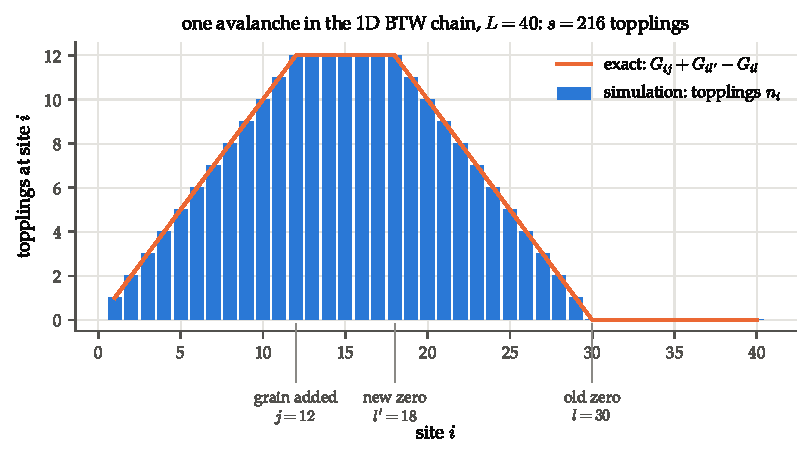
\includegraphics[width=\linewidth]{soc/btw1d_profile.pdf}
  \caption{Number of topplings at each site in one avalanche of the chain with $L=40$, $l=30$, $j=12$. Bars: simulation.
  Line: \cref{eq:n1d}. The profile is made of straight segments with kinks at the three special sites.}
  \label{fig:btw1d-profile}
\end{figure}

\subsection{The distribution of avalanche sizes}

In the stationary state each pair $(l,j)$ occurs with probability $\frac{1}{L+1}\cdot\frac1L$, so \cref{eq:s1d} determines
the whole size distribution. Its mean follows quickly: as $l$ runs over its $L+1$ values, so does $l' = (l-j)\bmod(L+1)$, so the
averages of $g(l')$ and $g(l)$ are equal and cancel, leaving
\begin{equation}
  \avg{s} = \avg{g(j)} = \frac1L\sum_{j=1}^{L}\frac{j(L+1-j)}{2} = \frac{(L+1)(L+2)}{12},
\end{equation}
in agreement with Ruelle and Sen~\cite{RuelleSen1992} and with \cref{eq:mean-s}.

To see the \emph{shape} of the distribution, let $L$ be large and measure positions in units of $L$: $x = j/L$ and
$\lambda = l/L$ are then independent and uniformly distributed between 0 and 1. Since $g(m)/L^2\to\tfrac12\,\tfrac mL(1-\tfrac mL)$,
the natural variable is the size measured in units of $L^2$,
\begin{equation}
  y = \frac{s}{L^2} = \tfrac12\left[x(1-x) + \lambda'(1-\lambda') - \lambda(1-\lambda)\right],
\end{equation}
where $\lambda' = l'/L$. By \cref{eq:zero-moves} there are two cases.
\begin{itemize}
  \item If $\lambda > x$ (the empty site is to the right of the added grain), then $\lambda' = \lambda - x$. Expanding,
    \begin{align*}
      x(1-x) + (\lambda-x)(1-\lambda+x) - \lambda(1-\lambda)
      &= x - x^2 + \lambda - \lambda^2 + 2\lambda x - x - x^2 - \lambda + \lambda^2 \\
      &= 2x(\lambda - x),
    \end{align*}
    so $y = x\,(\lambda-x)$.
  \item If $\lambda < x$, then $\lambda' = \lambda - x + 1$, and the same algebra gives $y = (1-x)(x-\lambda)$.
\end{itemize}
The second case is the mirror image of the first (replace $x\to1-x$, $\lambda\to1-\lambda$), so the two contribute equally to the
distribution. Consider the first. For a fixed $x$, the variable $u = \lambda - x$ is uniform on $[0,1-x]$, so $y = xu$ is uniform on
$[0,\,x(1-x)]$ and has density $1/x$ there. A given value $y$ can be produced only by those $x$ with $x(1-x)>y$, i.e.\ by
$x_-<x<x_+$ with $x_\pm = \tfrac12\bigl(1\pm\sqrt{1-4y}\bigr)$. Integrating over these $x$ and doubling for the mirror case,
\begin{equation}
  \boxed{\; f(y) = 2\int_{x_-}^{x_+}\frac{\dd x}{x} = 2\ln\frac{x_+}{x_-} = 2\ln\frac{1+\sqrt{1-4y}}{1-\sqrt{1-4y}},\qquad 0<y<\tfrac14. \;}
  \label{eq:fy}
\end{equation}
This is the result of Ruelle and Sen~\cite{RuelleSen1992}, here obtained in a more elementary way. The largest possible value $y=1/4$
corresponds to $x = 1/2$, $\lambda=1$: a grain added in the middle of the chain when the empty site is at the far end. Near $y=0$ the
density has a mild (logarithmic) divergence, and near $y = 1/4$ it goes to zero like a square root. Ruelle and Sen also found that the
duration, measured in units of $L$, has the density $2t$ on $0<t<1$. \Cref{fig:btw1d-dist} compares both results with simulations.

\begin{figure}[t]
  \centering
  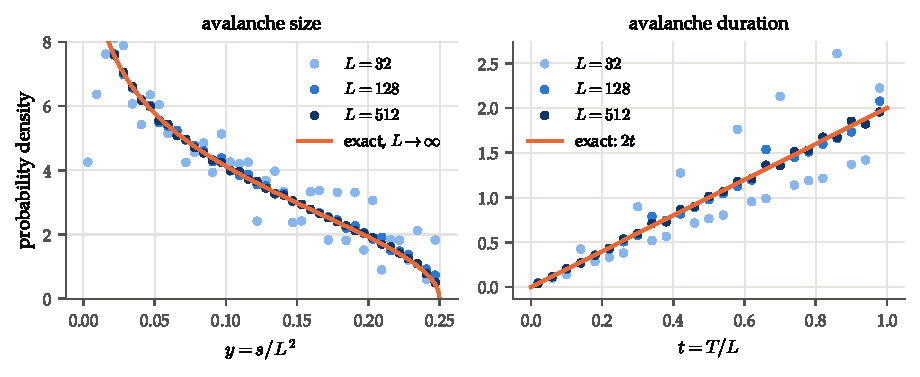
\includegraphics[width=\linewidth]{soc/btw1d_distribution.pdf}
  \caption{The one-dimensional sandpile. Left: density of the scaled avalanche size $s/L^2$ from simulations with $L = 32$, 128 and
  512 (points), and the exact large-$L$ result \cref{eq:fy} (line). Right: density of the scaled duration $T/L$ and the exact result
  $2t$. The points for $L=32$ scatter because $s$ takes only integer values. The curves for different $L$ coincide after the rescaling:
  the only scale in the problem is the system size.}
  \label{fig:btw1d-dist}
\end{figure}

\subsection{What the one-dimensional solution means}

The one-dimensional sandpile is ``critical'' only in a restricted sense. Avalanches of all sizes up to the system size occur, and there
is no length scale other than $L$. But the size distribution is \emph{not a power law}. It has the form
\begin{equation}
  P(s) = \frac{1}{L^2}\, f\!\left(\frac{s}{L^2}\right),
\end{equation}
so almost all avalanches have sizes of order $L^2$; there is no range of sizes in which $P(s)\propto s^{-\tau}$ with $\tau>1$. Compared with
\cref{eq:fss}, this corresponds to $D=2$ and an exponent $\tau=0$, and the relation \cref{eq:scaling-relation} does not apply because it
assumed $\tau>1$. The situation is similar to one-dimensional percolation (\cref{sec:perc1d}): in one dimension a single empty site can stop
or redirect an avalanche, and the critical state is too simple to produce scale-free behaviour.

This has a practical lesson for the analysis of data. Over one or two decades, a distribution like \cref{eq:fy} can look roughly straight
on a log--log plot. A straight piece of a log--log plot is therefore not proof of a power law. The reliable test is to change the system
size: a true power law extends to larger sizes with the \emph{same} slope, while a distribution like \cref{eq:fy} simply shifts as a whole.
Chapter~3 develops this into a systematic method.

% ======================================================================
\section{The two-dimensional sandpile}
\label{sec:btw2d}

On the square lattice ($k=4$, $z_c=4$, heights $0,\dots,3$) the BTW model is genuinely critical, but its exponents are not known exactly.
We present simulations with $L$ from 32 to $\socLmax$, with $\socNav$ avalanches for each $L$ after the system has reached its stationary
state. The simulation program is described in Chapter~6. We first compare with the exact results that do exist, then examine the avalanches,
and finally measure the exponents.

\subsection{Comparison with exact results}

\paragraph{Height probabilities.} For an infinitely large lattice, the probability that a site in the stationary state has height 0 was
calculated exactly by Majumdar and Dhar~\cite{MajumdarDhar1991},
\begin{equation}
  P_0 = \frac{2}{\pi^2} - \frac{4}{\pi^3} \approx 0.0736 .
\end{equation}
The probabilities of the other heights were obtained later~\cite{Priezzhev1994,JengPirouxRuelle2006}, and the mean height is exactly
$17/8 = 2.125$. (The literature uses heights $1,\dots,4$; we subtract 1.) \Cref{tab:heights} compares them with our simulation on a
$\socLmax\times\socLmax$ lattice, measured on its central part to avoid the influence of the edges. The agreement is to the third decimal.

\begin{table}[t]
\centering
\caption{Probability of each height in the stationary state of the two-dimensional BTW model.}
\label{tab:heights}
\begin{tabular}{lccccc}
\toprule
height & 0 & 1 & 2 & 3 & mean \\
\midrule
exact, infinite lattice & 0.0736 & 0.1739 & 0.3063 & 0.4462 & 2.1250 \\
simulation, $L=\socLmax$ & \socHeightSim{0} & \socHeightSim{1} & \socHeightSim{2} & \socHeightSim{3} & \socMeanHeightSim \\
\bottomrule
\end{tabular}
\end{table}

\paragraph{Mean avalanche size.} \Cref{eq:mean-s} can be evaluated for each $L$ by solving one linear system. For $L=\socLmax$ it gives
$\avg{s} = \socMeanExact$, and the simulation gives $\socMeanSim$. \Cref{fig:btw2d-moments} (left) shows the comparison for all $L$:
$\avg{s}$ grows as $L^2$, as \cref{eq:mean-L2} requires, and the simulation agrees with the exact value at every size.

\subsection{The avalanches}

\Cref{fig:btw2d-snapshot} shows one large avalanche. The region that toppled is compact, and the number of topplings per site increases in
nested, roughly concentric layers towards the site where the grain was added. Each layer corresponds to a ``wave'': the starting site
topples, a wave of topplings spreads out, and when it has died the starting site may be unstable again and start the next wave. Priezzhev,
Ktitarev and Ivashkevich~\cite{Priezzhev1996} showed that single waves are much simpler objects than whole avalanches (the exponent of their
size distribution, $11/8$, can be calculated exactly), and that the difficulty of the BTW model lies in how waves stack up into avalanches.

\begin{figure}[t]
  \centering
  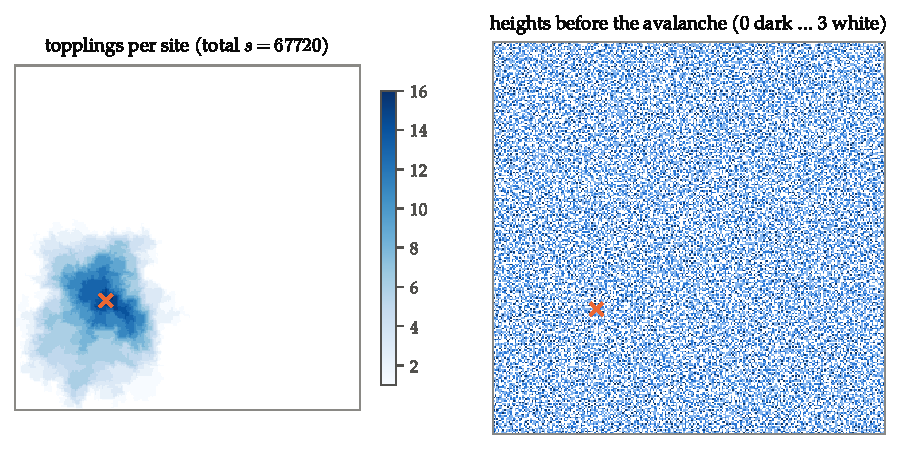
\includegraphics[width=\linewidth]{soc/btw2d_snapshot.pdf}
  \caption{One large avalanche on a $256\times256$ lattice; the grain was added at the site marked $\times$. Left: number of topplings at each
  site. Right: the heights just before the grain was added.}
  \label{fig:btw2d-snapshot}
\end{figure}

\Cref{fig:btw2d-dist} shows the distributions of size, area and duration. Unlike in one dimension, each distribution has a straight
section on the log--log plot whose slope \emph{does not change} with $L$; increasing $L$ only extends the straight section to larger
values, as in \cref{eq:fss}. This is the signature of genuine critical behaviour. A guide line with slope $-1.2$ is drawn for the size
distribution, but its local slope drifts slowly, and fitting a straight line by eye is not a reliable way to obtain $\tau$.

\begin{figure}[t]
  \centering
  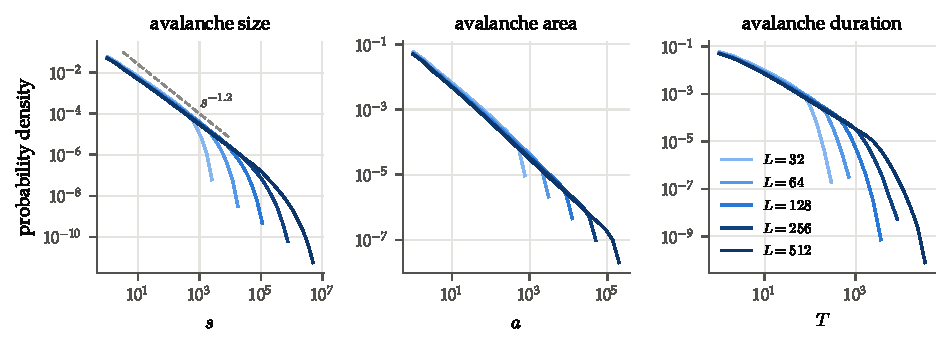
\includegraphics[width=\linewidth]{soc/btw2d_distributions.pdf}
  \caption{Two-dimensional BTW sandpile: probability densities of avalanche size, area and duration for $L = 32$, 64, 128, 256 and 512
  (light to dark). Logarithmically spaced bins are used so that each decade has the same number of points.}
  \label{fig:btw2d-dist}
\end{figure}

\subsection{Measuring the exponents with moments}

A more reliable method uses the moments of the distribution instead of its shape. Assume the form \cref{eq:fss},
$P(s) = s^{-\tau}\mathcal G(s/s_c)$ with $s_c = c\,L^{D}$. The $q$-th moment is
\begin{equation}
  \avg{s^q} = \int s^{q}\, s^{-\tau}\,\mathcal G\!\left(\frac{s}{s_c}\right)\dd s .
\end{equation}
Substitute $s = s_c u$, $\dd s = s_c\,\dd u$:
\begin{equation}
  \avg{s^q} = s_c^{\,q+1-\tau}\int u^{q-\tau}\,\mathcal G(u)\,\dd u \;\propto\; L^{D(q+1-\tau)} .
\end{equation}
The remaining integral is a number independent of $L$, provided $q>\tau-1$ so that it converges at small $u$ (for smaller $q$ the small
avalanches dominate and the moment does not grow with $L$). Defining the \emph{moment exponent} $\sigma(q)$ by $\avg{s^q}\propto L^{\sigma(q)}$,
\begin{equation}
  \sigma(q) = D\,(q+1-\tau) .
  \label{eq:moments}
\end{equation}
So $\sigma(q)$ is a straight line in $q$ with slope $D$. Each $\sigma(q)$ is measured as the slope of $\log\avg{s^q}$ against $\log L$. This uses
all the data, requires no binning and no choice of a fitting window in $s$. As a check, $\sigma(1) = D(2-\tau)$ must equal 2 by
\cref{eq:scaling-relation}.

\Cref{fig:btw2d-moments} (right) shows the measured $\sigma(q)$. The value at $q=1$ is 2, as it must be, and the slope for $q\ge2$ gives
$D\approx\socDest$. With \cref{eq:scaling-relation}, $\tau = 2-2/D \approx \socTauRel$. Large-scale simulations by Lübeck and
Usadel~\cite{LubeckUsadel1997} give $\tau\approx1.29$ and $D\approx2.73$. Our $\tau$ agrees; our $D$ is about 3\% larger, which is not
surprising for system sizes up to $\socLmax$ and a slope estimated from three sizes. Part of the difference, however, is a real property of
the model: on close inspection $\sigma(q)$ is not exactly a straight line. Tebaldi, De Menech and Stella~\cite{Tebaldi1999} showed that the BTW
model does not follow the simple form \cref{eq:fss} exactly: small and large avalanches scale with slightly different exponents, a property
called \emph{multifractality}. For the BTW model, therefore, ``the'' value of $\tau$ depends somewhat on how it is measured. Other sandpile
models, such as the stochastic Manna model, follow \cref{eq:fss} much more cleanly.

\begin{figure}[t]
  \centering
  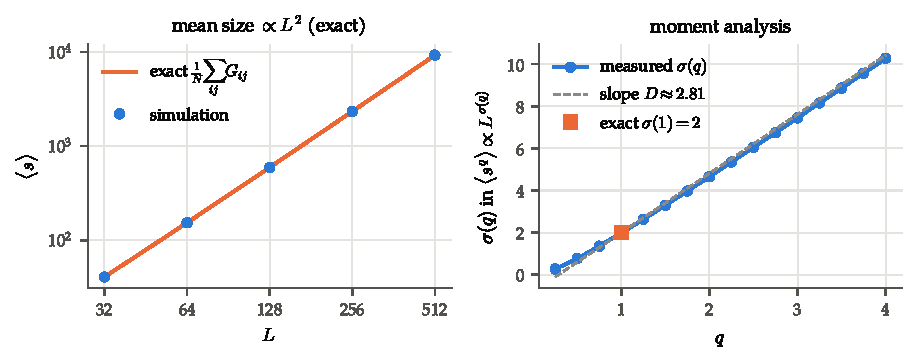
\includegraphics[width=\linewidth]{soc/btw2d_moments.pdf}
  \caption{Two-dimensional BTW sandpile. Left: mean avalanche size against $L$; the line is the exact \cref{eq:mean-s}, the points are
  simulations. Right: moment exponents $\sigma(q)$, obtained from the three largest system sizes; the dashed line has the slope $D$ fitted for
  $q\ge2$, and the square marks the exact value $\sigma(1)=2$.}
  \label{fig:btw2d-moments}
\end{figure}

% ======================================================================
\section{Summary and implications for the Burridge--Knopoff model}
\label{sec:soc-implications}

The main points of this chapter are:
\begin{itemize}
  \item A power law $P(x)\propto x^{-\tau}$ is the only distribution without a characteristic scale. In ordinary statistical physics it appears
    only at a critical point, which must be reached by tuning a control parameter.
  \item Self-organized criticality is the proposal that slow driving, a local threshold, fast local relaxation and dissipation drive a system to
    its critical point without tuning. The feedback argument of \cref{sec:soc} shows why, and also that it requires the limits of vanishing
    driving rate and vanishing bulk dissipation.
  \item The BTW sandpile is Abelian. This gives exact results: all recurrent configurations are equally likely, the mean number of topplings is
    the Green function, $\avg{s}\propto L^2$, and $D(2-\tau)=2$.
  \item In one dimension the BTW model is solved exactly: an added grain moves the single empty site by $j$ places, the avalanche size is
    $s = g(j) + g(l') - g(l)$, and the size distribution is a function of $s/L^2$ that is \emph{not} a power law.
  \item In two dimensions the BTW model is critical, with $\tau\approx1.2$--$1.3$ and $D\approx2.7$--$2.8$, and small deviations from simple
    scaling.
\end{itemize}

Three of these points shape the rest of this thesis.

\emph{One dimension.} The Burridge--Knopoff model studied here is one-dimensional, and the simplest one-dimensional sandpile is not
critical. Whatever broad distribution of event sizes the Burridge--Knopoff model produces must therefore come from features that the
one-dimensional BTW model does not have: continuous rather than integer variables, deterministic rather than random driving, or the inertia of
the blocks.

\emph{Bulk dissipation.} In the sandpile, grains are lost only at the edges, and this is what makes $\avg{s}\propto L^2$ and the cutoff grow with
the system size. In the Burridge--Knopoff model every block is attached to the moving plate by a pulling spring. When a block slips, part of the
force it releases goes into its own pulling spring rather than to its neighbours, so stress is lost \emph{inside} the system. In the language of
the random-walk picture of \cref{sec:mean}, a grain that is lost with probability $\epsilon$ at each step travels on average only a distance of
order $\epsilon^{-1/2}$ before it disappears. Such bulk dissipation introduces a length scale that does not depend on $L$, and avalanches larger
than this scale are suppressed. For the Burridge--Knopoff model this length turns out to be set by the ratio of the two spring constants,
$\ell = \sqrt{k_c/k_p}$, as will be shown in Chapters~4 and~5.

\emph{Uniform driving.} In the sandpile, grains are added at random sites; in the Burridge--Knopoff model the plate loads all blocks
simultaneously and deterministically. The model that combines continuous variables, uniform driving and bulk dissipation is the
Olami--Feder--Christensen model~\cite{OFC1992}, which will be the starting point of the mapping in Chapter~5.

\chapter{Measuring exponents from finite data}
\label{ch:measuring}

\newcommand{\stestLSlinMean}{0.893}
\newcommand{\stestLSlinStd}{0.124}
\newcommand{\stestLSlogMean}{1.907}
\newcommand{\stestLSlogStd}{0.080}
\newcommand{\stestLScumMean}{1.992}
\newcommand{\stestLScumStd}{0.032}
\newcommand{\stestMLEMean}{2.000}
\newcommand{\stestMLEStd}{0.023}
\newcommand{\stxminBest}{10.0}
\newcommand{\stxminTau}{2.496}
\newcommand{\stxminErr}{0.011}
\newcommand{\stxminTauOne}{1.58}
\newcommand{\stbtwWinTau}{1.123}
\newcommand{\stbtwWinErr}{0.002}
\newcommand{\stbtwWinP}{0.15}
\newcommand{\stcorrRatio}{0.2}
\newcommand{\stcorrAcfOne}{-0.007}
\newcommand{\stcorrSeed}{0.14}
\newcommand{\stsynTau}{1.608}
\newcommand{\stsynD}{2.056}
\newcommand{\stsynCost}{0.8}
\newcommand{\stmomD}{2.81}
\newcommand{\stmomTau}{1.29}
\newcommand{\stmomCost}{1197}
\newcommand{\stcollATau}{1.15}
\newcommand{\stcollAD}{2.21}
\newcommand{\stcollACost}{109}
\newcommand{\stcollBTau}{1.69}
\newcommand{\stcollBD}{3.21}
\newcommand{\stcollBCost}{3}
\newcommand{\stDloc}{2.70, 2.69, 2.88, 2.73}
\newcommand{\stDerr}{0.02, 0.04, 0.05, 0.08}


The previous chapter showed that the central claims about a critical system are statements about
exponents: the exponent $\tau$ of the size distribution, the exponent $D$ that says how the cutoff
grows with the system size. A simulation produces a finite list of numbers, and turning that list
into an exponent with an honest error bar is harder than it looks. Three difficulties appear in
every case:
\begin{enumerate}[nosep]
  \item \textbf{Statistical noise.} Large events are rare, so the tail of a distribution is always
    poorly sampled.
  \item \textbf{A finite range.} The power law holds only between a lower scale (the lattice, one
    block) and an upper cutoff (the system size, the correlation length). Outside this range the
    distribution bends, and a fit that ignores this is biased.
  \item \textbf{A finite system.} Even inside the range, the exponents measured at finite size
    differ from their asymptotic values by \emph{corrections to scaling} that disappear only slowly.
\end{enumerate}
A fourth, more technical difficulty is that consecutive events in a simulation are not independent.

This chapter develops the methods used in the rest of the thesis to deal with these problems. To
know whether a method works, it must be tried on data whose answer is known. We therefore test every
method first on \emph{synthetic data}, random numbers drawn from a distribution chosen by us, and then
apply it to the two-dimensional BTW sandpile of Chapter~\ref{ch:soc}. The methods follow
Clauset, Shalizi and Newman~\cite{Clauset2009}, Newman~\cite{Newman2005}, and the standard literature on
finite-size scaling. The chapter ends (\cref{sec:protocol}) with the procedure adopted for the
Burridge--Knopoff model.

% ======================================================================
\section{Estimating a probability density: histograms}
\label{sec:histograms}

\subsection{Counts and densities}

Suppose we have $N$ measured values $x_1,\dots,x_N$ (for example, the sizes of $N$ avalanches). To estimate
the probability density $P(x)$, divide the $x$-axis into intervals called \emph{bins}, with edges
$e_0<e_1<\dots$, and count the number $n_k$ of values that fall into bin $k$, the interval $[e_k,e_{k+1})$.
The fraction $n_k/N$ estimates the probability of falling into the bin, which is $\int_{e_k}^{e_{k+1}}P(x)\,\dd x
\approx P(x)\,w_k$, where $w_k = e_{k+1}-e_k$ is the width of the bin. Hence
\begin{equation}
  \hat P(x_k) = \frac{n_k}{N\,w_k}
  \label{eq:hist}
\end{equation}
is an estimate of the density at a point $x_k$ inside the bin. Dividing by the width is essential: without
it, wider bins would show more counts simply because they are wider.

\paragraph{The error of a bin.} Each of the $N$ values falls into bin $k$ with a small probability, independently
of the others. The number $n_k$ is then (to a very good approximation) a \emph{Poisson} random variable, whose
standard deviation is the square root of its mean. The statistical error of a bin is therefore
\begin{equation}
  \delta n_k \approx \sqrt{n_k}, \qquad \frac{\delta\hat P}{\hat P} = \frac{1}{\sqrt{n_k}}.
\end{equation}
A bin with 100 counts is known to 10\%; a bin with one count is known only to within a factor of two or so.

\subsection{Linear and logarithmic bins}

The simplest choice is bins of equal width. For a power law this is a poor choice (\cref{fig:binning}, left).
Because $P(x)$ falls by many orders of magnitude, the bins in the tail contain zero or one event. Bins with
zero events cannot even be drawn on a logarithmic axis, and those with one event pile up on a horizontal line
at $\hat P = 1/(Nw)$: the ``floor'' of the histogram. This floor has nothing to do with the true distribution.

\begin{figure}[t]
  \centering
  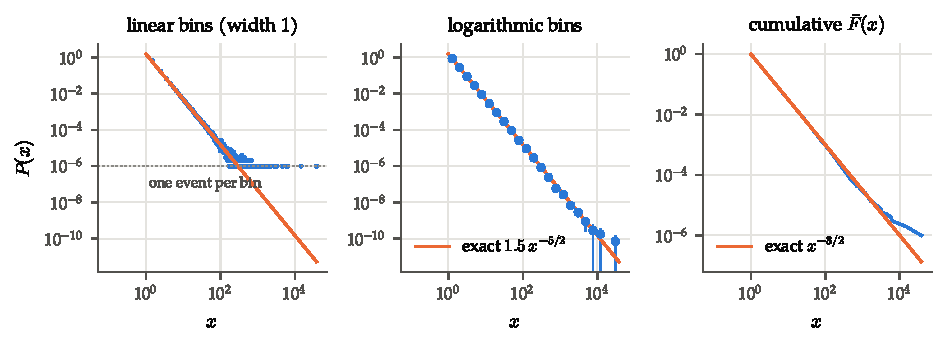
\includegraphics[width=\linewidth]{stats/binning.pdf}
  \caption{One million values drawn from the power law $P(x) = 1.5\,x^{-5/2}$, $x\ge1$, shown in three ways.
  Left: bins of width 1; the tail is dominated by bins with a single event (dotted line). Middle: logarithmic
  bins, five per decade, with Poisson error bars. Right: the complementary cumulative distribution, which needs
  no bins.}
  \label{fig:binning}
\end{figure}

The remedy is \emph{logarithmic binning}: bins whose edges are equally spaced in $\log x$,
\begin{equation}
  e_k = x_{\min}\, 10^{k/m},
\end{equation}
with $m$ bins per decade. The width of a bin is then proportional to its position, $w_k\propto e_k$, so bins in
the tail are wide and collect many events. For a power law the expected count in a bin is
$N P(x) w \propto x^{-\tau}\cdot x = x^{1-\tau}$, which falls much more slowly than $P(x)$ itself. On a log--log
plot the bins are equally spaced, and the points have comparable error bars over many decades
(\cref{fig:binning}, middle).

For \emph{integer} data such as numbers of topplings, the edges must be rounded to integers, and the width $w_k$ in
\cref{eq:hist} is the number of integers in the bin; otherwise the first few bins, which contain only one or two
integers, are distorted.

\paragraph{The magnitude histograms of Carlson and Langer.} Carlson and Langer plot the frequency of events as a
function of $\mu = \ln M$, using bins of equal width in $\mu$. Equal bins in $\ln M$ are exactly logarithmic bins in
$M$. Their density per unit $\mu$ is $\mathcal R(\mu) = M P(M)$ (\cref{eq:CL-b-tau}), so for a power law
$\mathcal R \propto M^{1-\tau} = e^{-(\tau-1)\mu}$. A straight line of slope $-b$ in their plots therefore
corresponds to
\begin{equation}
  \tau = 1 + b ,
\end{equation}
as found in Chapter~\ref{ch:intro}.

\subsection{The cumulative distribution}

The complementary cumulative distribution $\bar F(x)$ is estimated without any binning: sort the values, and for
the $r$-th smallest value set $\hat{\bar F}(x_{(r)}) = (N-r+1)/N$, the fraction of values at least as large.
For a power law $\bar F\propto x^{-(\tau-1)}$ (\cref{eq:Fbar-pl}), a straight line on a log--log plot
(\cref{fig:binning}, right). The cumulative plot is smooth and is very useful to judge by eye whether the tail
follows a power law. Its points are, however, strongly correlated with each other, since each point counts all
the values above it; this matters when a line is fitted through them.

% ======================================================================
\section{Why straight-line fits on log--log plots fail}
\label{sec:ls}

The most common way to estimate an exponent is to fit a straight line through the points of a log--log plot by
least squares and read off the slope. Least squares is the right method when the points are independent and have
Gaussian errors of the same size. None of these conditions holds here:
\begin{itemize}[nosep]
  \item the relative error of a histogram bin, $1/\sqrt{n_k}$, varies by orders of magnitude between the
    head and the tail, and the error of $\log n_k$ is not Gaussian when $n_k$ is small;
  \item empty bins must be discarded (their logarithm is $-\infty$), which removes precisely the bins that are
    below average and biases the tail upwards;
  \item the points of a cumulative plot are not independent.
\end{itemize}

To see how much this matters, we drew 1000 independent samples of $N=2000$ values each from a power law with
$\tau = 2$ and $x_{\min}=1$, and estimated $\tau$ in four ways for every sample. The results are shown in
\cref{fig:estimators}:

\begin{center}
\begin{tabular}{lcc}
\toprule
method & mean of $\hat\tau$ & spread (std) \\
\midrule
least squares, linear bins of width 1 & \stestLSlinMean & \stestLSlinStd \\
least squares, logarithmic bins & \stestLSlogMean & \stestLSlogStd \\
least squares, cumulative distribution & \stestLScumMean & \stestLScumStd \\
maximum likelihood (\cref{sec:mle}) & \stestMLEMean & \stestMLEStd \\
\bottomrule
\end{tabular}
\end{center}

\begin{figure}[t]
  \centering
  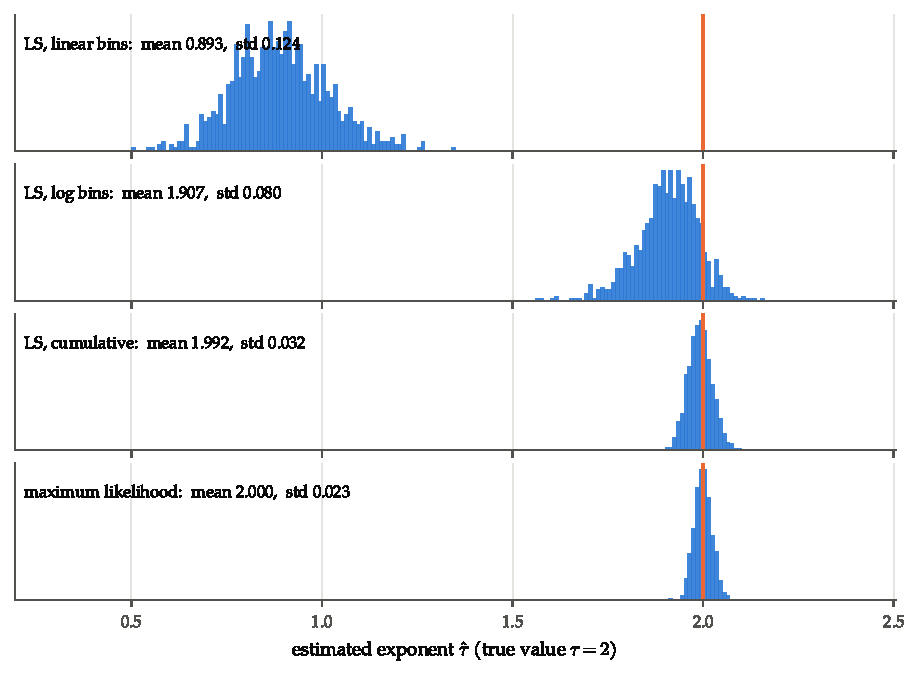
\includegraphics[width=\linewidth]{stats/estimators.pdf}
  \caption{Estimates of $\tau$ from 1000 independent synthetic samples of 2000 values with true exponent $\tau=2$
  (vertical line), using four methods.}
  \label{fig:estimators}
\end{figure}

Least squares on a linear histogram is useless: it does not even get close to the right answer. With logarithmic
bins the result is biased by about 5\%, and the spread is large. The cumulative distribution does better, but the
maximum-likelihood method, described next, is both unbiased and the most precise.

% ======================================================================
\section{Maximum likelihood}
\label{sec:mle}

\subsection{The idea}

Suppose we have a model for the distribution, $P(x\,|\,\tau)$, that depends on an unknown parameter $\tau$. For a
given value of $\tau$, the probability (density) of having observed exactly our data $x_1,\dots,x_N$ is, if the values are
independent,
\begin{equation}
  \mathcal L(\tau) = \prod_{i=1}^N P(x_i\,|\,\tau).
\end{equation}
Seen as a function of $\tau$, this is called the \emph{likelihood}. The \emph{maximum-likelihood estimate} $\hat\tau$ is the
value of $\tau$ that makes the observed data most probable. It is usually easier to maximise the logarithm,
$\ln\mathcal L = \sum_i \ln P(x_i\,|\,\tau)$, which has its maximum at the same place.

\subsection{Continuous power law}

For the normalised power law $P(x) = \frac{\tau-1}{x_{\min}}\left(\frac{x}{x_{\min}}\right)^{-\tau}$ on $x\ge x_{\min}$,
\begin{equation}
  \ln\mathcal L(\tau) = N\ln(\tau-1) - N\ln x_{\min} - \tau\sum_{i=1}^N \ln\frac{x_i}{x_{\min}} .
\end{equation}
Setting the derivative with respect to $\tau$ to zero,
\begin{equation}
  \frac{\dd\ln\mathcal L}{\dd\tau} = \frac{N}{\tau-1} - \sum_i\ln\frac{x_i}{x_{\min}} = 0
  \quad\Longrightarrow\quad
  \boxed{\;\hat\tau = 1 + \frac{N}{\sum_{i=1}^N \ln(x_i/x_{\min})}.\;}
  \label{eq:mle}
\end{equation}

\paragraph{Intuition.} Change variables to $u = \ln(x/x_{\min})$, the logarithm of the size. Since $\dd u = \dd x/x$,
\[
  P(u) = P(x)\frac{\dd x}{\dd u} = x\,P(x) = (\tau-1)\left(\frac{x}{x_{\min}}\right)^{1-\tau} = (\tau-1)\,e^{-(\tau-1)u}.
\]
The logarithm of a power-law variable is \emph{exponentially} distributed, with mean $1/(\tau-1)$. \Cref{eq:mle} simply
says: estimate $\tau-1$ as one over the average of $\ln(x/x_{\min})$. Every value contributes, each with the same weight;
nothing is binned and nothing is thrown away.

\paragraph{The error.} The width of the peak of $\ln\mathcal L$ tells how well $\tau$ is determined: a sharp peak means
that values of $\tau$ slightly different from $\hat\tau$ make the data much less probable. For large $N$, $\ln\mathcal L$
is close to a parabola near its maximum, and the standard error is
\begin{equation}
  \sigma_\tau = \left(-\frac{\dd^2\ln\mathcal L}{\dd\tau^2}\right)^{-1/2} = \left(\frac{N}{(\tau-1)^2}\right)^{-1/2}
  = \frac{\hat\tau-1}{\sqrt N} .
  \label{eq:mle-err}
\end{equation}
The error decreases as $1/\sqrt N$, as for any average. We checked that this error bar is correct by repeating the fit
on 400 independent synthetic samples: the true value lies within $\pm\sigma_\tau$ of the estimate in $68\%$ of the cases,
as it should for a Gaussian error.

\subsection{Discrete data}

Avalanche sizes are integers, and for small sizes the continuous formula is wrong: it treats all values between 1 and 2 as
if they were spread over the interval, whereas the data sit exactly at 1. For integers the normalised power law is
\begin{equation}
  P(s) = \frac{s^{-\tau}}{\zeta(\tau, s_{\min})}, \qquad
  \zeta(\tau, s_{\min}) = \sum_{s=s_{\min}}^{\infty} s^{-\tau},
\end{equation}
where $\zeta(\tau, s_{\min})$ is the \emph{Hurwitz zeta function}, available in standard numerical libraries. The
log-likelihood
\begin{equation}
  \ln\mathcal L(\tau) = -N\ln\zeta(\tau,s_{\min}) - \tau\sum_i\ln s_i
\end{equation}
has no closed-form maximum, but it is easily maximised numerically, and the error again follows from its curvature. The
difference is not small: for $10^5$ integers drawn from $P(s)\propto s^{-1.7}$, $s\ge1$, the continuous formula gives
$\hat\tau=2.04$, while the discrete likelihood gives the correct $1.701\pm0.002$.

\subsection{Fitting a window: the truncated power law}

Real distributions follow a power law only up to a cutoff. If a fit assumes that the power law continues to infinity, the
missing tail is interpreted as a steeper decay, and $\hat\tau$ comes out too large. For $10^5$ values drawn from a power law
with $\tau=1.25$ that ends sharply at $x=1000$, the untruncated fit gives $\hat\tau = 1.40$. The correct procedure is to fit
only a window $[x_{\min}, x_{\max}]$ and to normalise the model on that window:
\begin{equation}
  P(x) = \frac{x^{-\tau}}{Z(\tau)}, \qquad Z(\tau) = \int_{x_{\min}}^{x_{\max}} x^{-\tau}\,\dd x =
  \frac{x_{\min}^{1-\tau} - x_{\max}^{1-\tau}}{\tau-1}
\end{equation}
(for integers, $Z = \zeta(\tau, s_{\min}) - \zeta(\tau, s_{\max}+1)$). With this model the same data give $1.249\pm0.002$.
A useful by-product is that in a window the exponent can take any value, also $\tau\le1$, which is impossible for an
untruncated power law.

% ======================================================================
\section{Where does the power law start? Goodness of fit}
\label{sec:xmin}

\subsection{Choosing the lower limit}

At small sizes, lattice effects make the distribution deviate from the power law. The lower limit $x_{\min}$ of the fit must
be chosen above this region. Choosing it by eye is subjective; a systematic method is to choose the $x_{\min}$ for which the
fitted power law is closest to the data~\cite{Clauset2009}. ``Closest'' is measured by the \emph{Kolmogorov--Smirnov (KS)
distance}
\begin{equation}
  D_{\mathrm{KS}} = \max_{x\ge x_{\min}}\left|\hat F(x) - F_{\text{model}}(x)\right| ,
\end{equation}
the largest vertical gap between the measured cumulative distribution of the data above $x_{\min}$ and that of the fitted
power law. For each candidate $x_{\min}$ we fit $\tau$ by maximum likelihood and compute $D_{\mathrm{KS}}$; the best $x_{\min}$ is
the one with the smallest distance.

\Cref{fig:xmin} shows how this works on synthetic data: an exponential ``body'' below $x=10$ followed by a power-law tail with
$\tau=2.5$. If the fit starts at $x_{\min}=1$, the body is mistaken for part of the power law and $\hat\tau = \stxminTauOne$.
The KS distance drops sharply at the true onset; its minimum is at $x_{\min}=\stxminBest$, where
$\hat\tau=\stxminTau\pm\stxminErr$. Above the onset, $\hat\tau$ is flat in $x_{\min}$ (right panel); a flat region of this kind is
itself a good sign that a power law is present.

\begin{figure}[t]
  \centering
  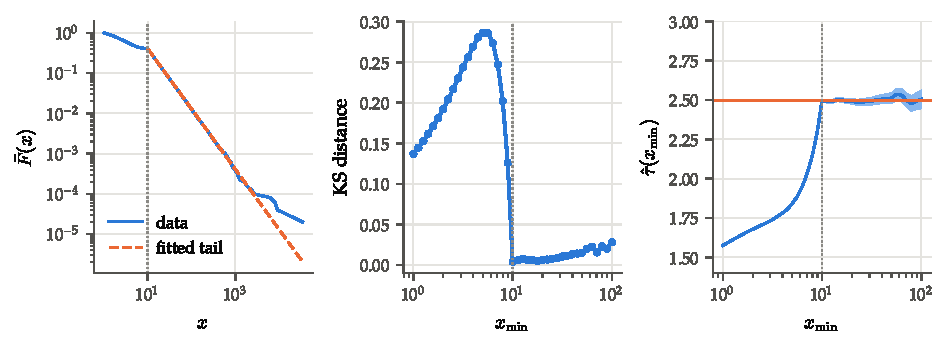
\includegraphics[width=\linewidth]{stats/xmin.pdf}
  \caption{Choosing $x_{\min}$. Synthetic data with an exponential body below 10 and a power-law tail with $\tau=2.5$. Left:
  cumulative distribution and the fitted tail. Middle: KS distance as a function of the lower limit. Right: fitted exponent with
  its error band; the horizontal line is the true value.}
  \label{fig:xmin}
\end{figure}

\subsection{Is it a power law at all?}

A fit always returns a number, even if the data do not follow a power law. To test the hypothesis itself we ask: if the data
really came from the fitted power law, how often would a sample of the same size have a KS distance as large as the one observed?
This probability, the $p$-value, is computed by a \emph{parametric bootstrap}~\cite{Efron1979,Clauset2009}:
\begin{enumerate}[nosep]
  \item fit the data, obtaining $\hat\tau$ and the observed distance $D_{\mathrm{obs}}$;
  \item draw many synthetic samples, of the same size, from the power law with exponent $\hat\tau$;
  \item fit each synthetic sample in the same way and compute its KS distance;
  \item the $p$-value is the fraction of synthetic samples whose distance is at least $D_{\mathrm{obs}}$.
\end{enumerate}
If $p$ is small (we use $p<0.1$), data of this kind rarely come from a power law, and the hypothesis is rejected. A large $p$
does not prove that the distribution is a power law; it only says that the data are consistent with one.

% ======================================================================
\section{Statistical errors of correlated data}
\label{sec:correlated}

\subsection{Why independence fails}

The error formula $\sigma/\sqrt N$ for a mean assumes independent values. In a simulation of a sandpile or of a fault, events are
produced one after the other by the same system, and the state left behind by one event is the starting state of the next. Events
can therefore be correlated in time. The \emph{autocorrelation function}
\begin{equation}
  C(\Delta) = \frac{\avg{(x_t-\avg{x})(x_{t+\Delta}-\avg{x})}}{\avg{(x-\avg{x})^2}}
\end{equation}
measures how similar two events separated by $\Delta$ steps are; $C(0)=1$, and $C(\Delta)=0$ for independent events. For a series
of $N$ correlated values the variance of the mean is
\begin{equation}
  \mathrm{Var}(\bar x) = \frac{\sigma^2}{N}\Bigl(1 + 2\sum_{\Delta\ge1} C(\Delta)\Bigr),
  \label{eq:var-corr}
\end{equation}
so positive correlations increase the error and negative ones decrease it. Even very small correlations matter if they last
long, because \cref{eq:var-corr} sums them over all lags.

\subsection{The blocking method}

A practical way to obtain the correct error without computing $C(\Delta)$ is the \emph{blocking} method~\cite{FlyvbjergPetersen1989}.
Divide the series into consecutive blocks of length $b$, compute the mean of each block, and estimate the error of the overall
mean from the scatter of the block means as if they were independent. For $b=1$ this is the naive error. As $b$ grows beyond the
time over which events are correlated, the block means become independent, and the estimate stops changing: the value on this
\emph{plateau} is the correct error. For quantities other than the mean, such as exponents, the same idea leads to the \emph{block
bootstrap}: resample whole blocks (with replacement) many times, recompute the quantity each time, and use the spread of the
results as the error.

\subsection{An example: the BTW sandpile}

\Cref{fig:correlations} shows the autocorrelation of avalanche sizes in the two-dimensional BTW model with $L=64$. It is tiny,
$C(1)=\stcorrAcfOne$, but negative and long-lived. The blocking analysis (right) shows that the correct error of $\avg{s}$ is not
the naive one but only about $\stcorrSeed$ of it, a factor of seven smaller.

\begin{figure}[t]
  \centering
  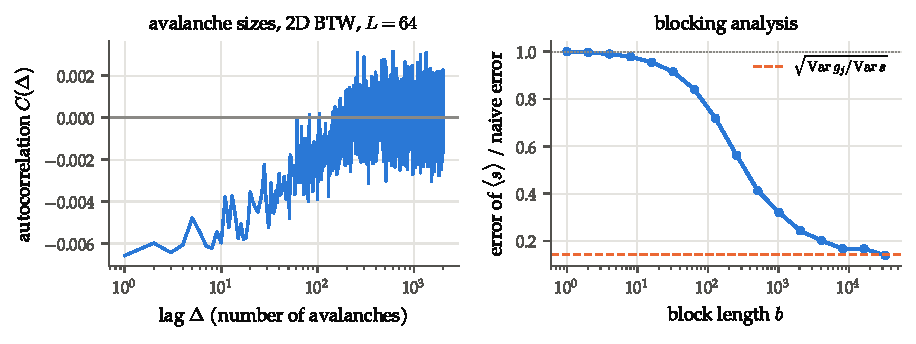
\includegraphics[width=\linewidth]{stats/correlations.pdf}
  \caption{Two-dimensional BTW model, $L=64$, $10^6$ avalanches. Left: autocorrelation of the sizes of consecutive avalanches.
  Right: error of the mean size from the blocking method, in units of the naive error $\sigma/\sqrt N$; the dashed line is the
  prediction of \cref{eq:block-sum}.}
  \label{fig:correlations}
\end{figure}

This surprising result has an exact explanation, which shows the power of the balance equation \cref{eq:balance}. Add up the balance
equations of $b$ consecutive grains, added at sites $j_1,\dots,j_b$. The heights at the end of the block are
\[
  z^{\text{end}} = z^{\text{start}} + \sum_{t=1}^b e_{j_t} - \Delta\,N_{\text{block}},
\]
where $N_{\text{block}}$ is the vector of the total numbers of topplings at each site during the block. Solving for $N_{\text{block}}$ with
$G=\Delta^{-1}$ and summing over sites,
\begin{equation}
  \sum_{t=1}^b s_t = \sum_{t=1}^b g_{j_t} + \sum_{i,m} G_{im}\bigl(z_m^{\text{start}} - z_m^{\text{end}}\bigr).
  \label{eq:block-sum}
\end{equation}
The second term is bounded, since all heights lie between 0 and 3; divided by $b$, it disappears for long blocks. The first term is a
sum of $b$ independent random numbers, because the sites $j_t$ are chosen independently. So for long blocks the fluctuation of the mean
size comes only from the randomness of \emph{where} grains are dropped, not from the avalanches themselves, and the error of the mean is
$\sqrt{\mathrm{Var}(g_j)/b}$ instead of $\sqrt{\mathrm{Var}(s)/b}$. For $L=64$ the ratio $\sqrt{\mathrm{Var}(g_j)/\mathrm{Var}(s)}$ is
$\stcorrSeed$, exactly the plateau of \cref{fig:correlations}. The anticorrelation has a simple physical meaning: an unusually large
avalanche removes many grains, and the following avalanches are smaller until the pile has been refilled.

This exact cancellation is special to a conservative sandpile, but the lesson is general: errors must always be estimated with a method
that accounts for correlations, such as blocking or the block bootstrap. Depending on the sign of the correlations, the naive error can be
too large or too small.

% ======================================================================
\section{Finite-size scaling}
\label{sec:fss}

\subsection{The scaling hypothesis}

In a finite system the power law is cut off at a size that grows with the system. The \emph{finite-size scaling} hypothesis states that
the system size $L$ is the \emph{only} scale in the problem besides the microscopic one, so that the distribution has the form
\begin{equation}
  P(s;L) = s^{-\tau}\,\mathcal G\!\left(\frac{s}{L^{D}}\right)
  \label{eq:fss3}
\end{equation}
for $s$ well above the lattice scale, with a cutoff function $\mathcal G$ that does not depend on $L$. This is the same form as the
percolation cluster distribution \cref{eq:perc-scaling}, with $L$ in place of the correlation length $\xi$: in a finite critical system,
the system size plays the role of the correlation length. In the Burridge--Knopoff model the roles will be reversed: the system can be made
much longer than the correlation length, and $\xi$ (set by the model parameters) will take the place of $L$.

\Cref{eq:fss3} has three consequences that can be tested with data from several system sizes.

\subsection{Data collapse}

Multiply \cref{eq:fss3} by $s^\tau$:
\begin{equation}
  s^{\tau}P(s;L) = \mathcal G\!\left(\frac{s}{L^{D}}\right).
\end{equation}
The right-hand side depends on $s$ and $L$ only through the combination $s/L^D$. So if we plot $s^\tau P(s;L)$ against $s/L^{D}$ for
several $L$, with the correct $\tau$ and $D$, all curves fall on top of each other: the data \emph{collapse} onto the single curve
$\mathcal G$. With wrong exponents, the curves are shifted or tilted relative to each other.

To make this quantitative, we compare the rescaled curves on a common grid of $s/L^{D}$ and compute how far they are from their (error-weighted)
mean, in units of their statistical errors~\cite{BhattacharjeeSeno2001}:
\begin{equation}
  \chi^2 = \frac{1}{N_{\text{grid}}}\sum_{\text{grid points}}\;\frac{1}{N_L-1}\sum_{L}\frac{\bigl(y_L - \bar y\bigr)^2}{\sigma_L^2},
\end{equation}
where $y_L = \ln[s^{\tau}P(s;L)]$ interpolated at the grid point, $\sigma_L$ its statistical error, $\bar y$ the weighted mean over the $N_L$
system sizes. If the curves agree within their statistical noise, $\chi^2\approx1$. The best exponents are those that minimise $\chi^2$. For
synthetic data with $\tau=1.6$ and $D=2$ (an exponential cutoff at $s = L^2$, $L$ from 32 to 256), this procedure gives
$\tau = \stsynTau$, $D=\stsynD$ with $\chi^2=\stsynCost$: a perfect collapse (\cref{fig:collapse}, left).

\subsection{Moments}

As derived in \cref{sec:btw2d}, \cref{eq:fss3} implies $\avg{s^q}\propto L^{\sigma(q)}$ with $\sigma(q) = D(q+1-\tau)$ for $q>\tau-1$. The
moment exponents are obtained as slopes of $\ln\avg{s^q}$ against $\ln L$, and their errors with the block bootstrap of
\cref{sec:correlated}. The slope of $\sigma(q)$ gives $D$, and its intercept gives $\tau$.

\subsection{Effective exponents}

Instead of fitting one exponent to all the data, it is often more informative to fit the truncated power law in a sliding window, for
example one decade $[s, 10s]$, and plot the resulting \emph{effective exponent} $\tau_{\text{eff}}$ against the position of the window.
For a true power law $\tau_{\text{eff}}$ is constant; deviations show where, and how strongly, the distribution bends.

\subsection{Corrections to scaling}

\Cref{eq:fss3} is an \emph{asymptotic} statement, valid for $L\to\infty$ and $s\to\infty$. At finite sizes there are corrections, and
when $\tau$ is close to 1 they can be surprisingly large. The reason is the normalisation. For \cref{eq:fss3} to be a normalised distribution
starting at $s=1$,
\[
  \int_1^\infty s^{-\tau}\mathcal G(s/s_c)\,\dd s \approx \frac{1}{\tau-1} - c\, s_c^{-(\tau-1)}
\]
must equal 1 for every $L$ (here $s_c = L^D$ and $c$ is a positive constant). The second term is a correction that decays as
$s_c^{-(\tau-1)}$. For $\tau=1.3$ this is $s_c^{-0.3}$: making the cutoff ten times larger reduces the correction only by a factor
$10^{0.3}\approx2$. To keep the distribution normalised, its overall amplitude must therefore change slowly with $L$, and all exponents
measured from a range of $L$ are affected.

\Cref{fig:corrections} shows this for a case where everything is known exactly: the moments of $P(s)\propto s^{-1.3}e^{-s/L^2}$, computed by
numerical integration. The local slopes $\dd\ln\avg{s^q}/\dd\ln L$ approach their asymptotic values $\sigma(q)=D(q+1-\tau)$ only slowly from
below; for $L$ around 30 the slope for $q=1$ is still about $10\%$ too small. A common way to handle this is to allow a correction term,
$\avg{s^q} = a\,L^{\sigma(q)}(1 + b\,L^{-\omega})$, or to compute effective exponents from pairs of neighbouring sizes and watch how they
change as $L$ grows.

\begin{figure}[t]
  \centering
  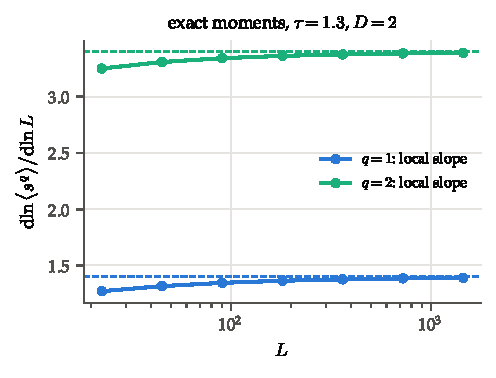
\includegraphics[width=0.55\linewidth]{stats/corrections.pdf}
  \caption{Corrections to scaling in a case known exactly: local slopes of the moments of $P(s)\propto s^{-1.3}e^{-s/L^2}$ between
  neighbouring system sizes (points), and their asymptotic values $D(q+1-\tau)$ (dashed lines).}
  \label{fig:corrections}
\end{figure}

% ======================================================================
\section{Application: the two-dimensional BTW sandpile}
\label{sec:btw2d-exponents}

We now apply these tools to the BTW data of \cref{sec:btw2d} ($L=32$ to 512, $10^6$ avalanches each). The results are a lesson in caution.

\paragraph{Effective exponents.} \Cref{fig:effective} (left) shows $\tau_{\text{eff}}$ from truncated fits in one-decade windows. For every $L$
there is a range in which $\tau_{\text{eff}}$ rises only slowly, from about $1.0$ to $1.13$, followed by a sharp rise at the cutoff. For
$L=512$, a fit of the window $[10^2,10^4]$ gives $\tau=\stbtwWinTau\pm\stbtwWinErr$ with a goodness-of-fit $p$-value of $\stbtwWinP$: in this
window the data are statistically consistent with a pure power law. The right panel shows what happens if the cutoff is ignored and all
$s\ge s_{\min}$ are fitted: $\hat\tau$ is always too large and keeps increasing with $s_{\min}$, so no stable value can be read off.

\begin{figure}[t]
  \centering
  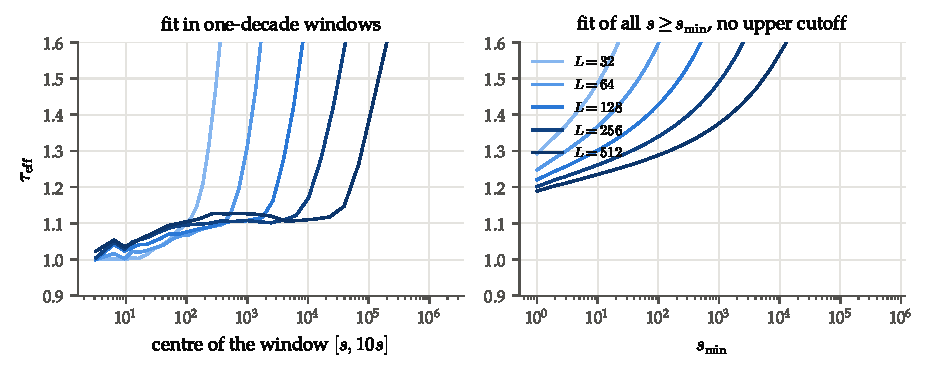
\includegraphics[width=\linewidth]{stats/effective_exponent.pdf}
  \caption{Effective exponents of the avalanche-size distribution of the two-dimensional BTW model. Left: truncated maximum-likelihood fits in
  windows $[s,10s]$, plotted at the centre of the window. Right: untruncated fits of all $s\ge s_{\min}$.}
  \label{fig:effective}
\end{figure}

\paragraph{Moments and collapse.} The moment analysis of \cref{sec:btw2d} gave $D=\stmomD$ and, through $D(2-\tau)=2$, $\tau=\stmomTau$, much
larger than the window value $1.12$. With these exponents the curves do not collapse (\cref{fig:collapse}, middle): their slopes at small $s/L^D$
differ visibly, and $\chi^2\approx\stmomCost$. Minimising $\chi^2$ over $\tau$ and $D$ does not rescue the collapse, and the result depends on which part
of the curves is used. Using the whole range gives $\tau=\stcollATau$, $D=\stcollAD$ ($\chi^2=\stcollACost$); using only the region near the cutoff
($s/L^D>10^{-2}$) gives $\tau=\stcollBTau$, $D=\stcollBD$ ($\chi^2=\stcollBCost$). Finally, the effective $D$ computed from pairs of neighbouring
sizes (\cref{fig:collapse}, right) is $\stDloc$ for the four pairs, with bootstrap errors $\stDerr$. These values scatter around the literature value
$2.73$~\cite{LubeckUsadel1997} but show no clear convergence.

\begin{figure}[t]
  \centering
  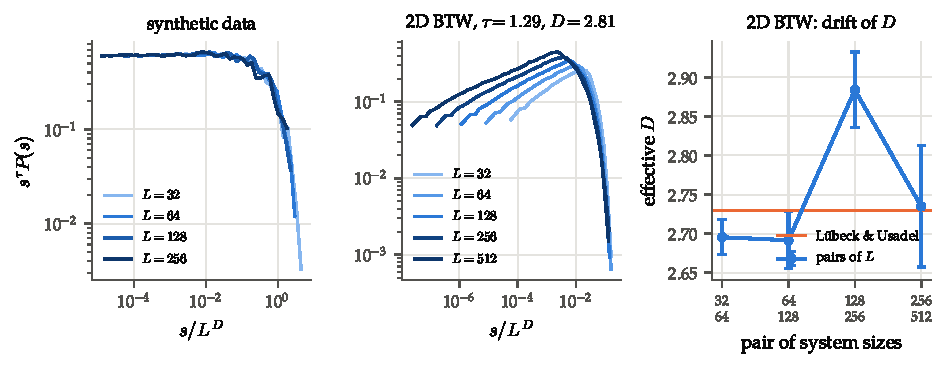
\includegraphics[width=\linewidth]{stats/collapse.pdf}
  \caption{Data collapse. Left: synthetic data that obey \cref{eq:fss3} exactly, collapsed with the fitted exponents. Middle: the two-dimensional
  BTW model, rescaled with the exponents from the moment analysis; the curves do not collapse. Right: effective fractal dimension $D$ of the BTW
  model obtained from pairs of neighbouring system sizes, with block-bootstrap errors, and the literature value.}
  \label{fig:collapse}
\end{figure}

\paragraph{Interpretation.} All the methods work correctly on synthetic data that obey \cref{eq:fss3}. Their disagreement on the BTW model is
therefore a property of the model, not of the methods: the BTW sandpile does not follow simple finite-size scaling. Small avalanches (single waves of
topplings) and large avalanches (many waves stacked on top of each other) scale differently, which is the multifractality mentioned in
\cref{sec:btw2d}~\cite{Tebaldi1999}. A single number $\tau$ cannot describe all scales, and different methods weight different scales. The general
lesson for this thesis is that an exponent should never be reported from one method alone: a value is trustworthy only when independent methods
(window fits, moments, collapse) agree within their errors.

% ======================================================================
\section{The procedure used in this thesis}
\label{sec:protocol}

For every model studied in the following chapters, distributions and exponents are obtained as follows.
\begin{enumerate}
  \item \textbf{Stationarity.} Start from a well-defined initial state, discard a transient long enough for averages to stop drifting, and record
    the events in time order.
  \item \textbf{Display.} Show densities with logarithmic bins (integer-aware for integer data) and Poisson error bars, and cumulative distributions
    for the tails. Magnitude histograms in $\mu=\ln M$ are translated with $\tau = 1+b$.
  \item \textbf{Exponents.} Estimate $\tau$ by maximum likelihood of a (discrete, if appropriate) truncated power law in a window. Choose the lower
    limit by the KS distance, test the fit with a bootstrap $p$-value, and show the effective exponent in sliding windows to make the range of validity
    visible.
  \item \textbf{Scaling.} Use several values of the parameter that sets the cutoff (the system size $L$ for sandpiles, the correlation length for the
    Burridge--Knopoff model). Measure moment exponents and test data collapse with the $\chi^2$ measure, and compute effective exponents from neighbouring
    values of the parameter to judge corrections to scaling.
  \item \textbf{Errors.} Estimate statistical errors with the block bootstrap. Report the spread between different methods as a systematic uncertainty.
  \item \textbf{Validation.} Before applying any analysis to new data, check that it returns the known answer on synthetic data generated with similar
    exponents, ranges and sample sizes.
\end{enumerate}

\chapter{The Burridge--Knopoff model}
\label{ch:bk}

This chapter presents the Burridge--Knopoff (BK) model in the form studied by Carlson,
Langer and collaborators~\cite{CarlsonLanger1989,Carlson1991}, and reviews their analysis.
We start from Newton's equations in physical units (\cref{sec:bk-eom}), reduce them to a
dimensionless form with only a few parameters (\cref{sec:bk-units}), and describe the two
friction laws used in the 1989 and 1991 papers (\cref{sec:bk-friction}). We then work out the
simplest motions of the model exactly (\cref{sec:bk-simple}), show why uniform sliding is
unstable (\cref{sec:bk-instability}), and follow Carlson and Langer's argument that leads to a
\emph{localization length}, the length that separates small, ``localized'' events from large,
``delocalized'' ones (\cref{sec:bk-pulses,sec:bk-localization}). The last part of the chapter
summarises the statistical results of the two papers, explains why they differ
(\cref{sec:bk-stats,sec:bk-differences}), and lists what a sandpile model would have to capture to
describe the BK model (\cref{sec:bk-summary}).

% ======================================================================
\section{Equations of motion}
\label{sec:bk-eom}

Consider the chain of \cref{fig:bk-sketch}: $N$ identical blocks of mass $m$, labelled
$j=1,\dots,N$, resting on a fixed rough surface. Let $X_j(t)$ be the displacement of block $j$ from
its position at time $t=0$, when all springs are relaxed. The upper plate moves with constant velocity
$v$, so at time $t$ it has moved by $vt$. Three kinds of forces act on block $j$:
\begin{itemize}
  \item \textbf{Coupling springs.} The spring to the right neighbour is stretched by $X_{j+1}-X_j$ and
    pulls block $j$ to the right with force $k_c(X_{j+1}-X_j)$; the spring to the left neighbour pulls
    with $k_c(X_{j-1}-X_j)$. Together:
    \begin{equation}
      k_c\,(X_{j+1} - 2X_j + X_{j-1}).
    \end{equation}
  \item \textbf{Pulling spring.} The leaf spring connecting the block to the plate is stretched by
    $vt - X_j$, the distance by which the plate has moved ahead of the block. It pulls the block
    forward with force $k_p\,(vt - X_j)$.
  \item \textbf{Friction.} The rough surface exerts a force $-F$ opposing the motion, described in
    \cref{sec:bk-friction}.
\end{itemize}
Newton's second law gives
\begin{equation}
  m\,\ddot X_j = k_c\,(X_{j+1} - 2X_j + X_{j-1}) + k_p\,(vt - X_j) - F_j ,
  \label{eq:bk-phys}
\end{equation}
where dots denote time derivatives. The first two terms together are the total \emph{spring force}
on the block, which we call $f_j$.

\paragraph{Boundary conditions.} Carlson and Langer use \emph{free} ends: the first and the last block
have only one coupling spring. This is expressed by defining $X_0\equiv X_1$ and $X_{N+1}\equiv X_N$ in
\cref{eq:bk-phys}, so that the missing spring exerts no force. (Setting $X_0 = X_{N+1}=0$ instead would
attach the end blocks to fixed walls, which is a different model.)

\paragraph{Friction.} The friction force depends on whether the block is moving:
\begin{itemize}
  \item A block at rest ($\dot X_j = 0$) is held by \emph{static} friction. Static friction takes whatever
    value is needed to keep the block at rest, $F_j = f_j$, as long as this is possible, i.e.\ as long as
    $f_j$ does not exceed the maximum static friction $F_0$. When $f_j$ reaches $F_0$, the block starts to
    slip.
  \item A slipping block feels \emph{kinetic} friction, which depends on its velocity:
    \begin{equation}
      F_j = F_0\,\phi\!\left(\frac{\dot X_j}{v_1}\right),
    \end{equation}
    where $\phi$ is a dimensionless function and $v_1$ is a characteristic velocity over which friction
    weakens. Since the surface is fixed, $\dot X_j$ is the velocity of the block relative to the surface.
\end{itemize}
A slipping block comes back to rest when its velocity returns to zero and the spring force is again within
the range that static friction can balance.

% ======================================================================
\section{Dimensionless form and the parameters of the model}
\label{sec:bk-units}

\Cref{eq:bk-phys} contains seven parameters: $m$, $k_c$, $k_p$, $F_0$, $v$, $v_1$ and the number of blocks
$N$. Many combinations of them give the same dynamics. To find the combinations that matter, we measure
time and displacement in natural units of the problem.

\paragraph{Unit of time.} A single block attached only to its pulling spring oscillates with angular
frequency $\omega_p = \sqrt{k_p/m}$. We use the dimensionless time
\begin{equation}
  \tau = \omega_p\, t .
\end{equation}

\paragraph{Unit of displacement.} A pulling spring exerts the maximum static friction force $F_0$ when it is
stretched by
\begin{equation}
  D_0 = \frac{F_0}{k_p} .
\end{equation}
This is the natural scale of slip: a block that slips releases a stretch of order $D_0$. We use the
dimensionless displacement $U_j = X_j/D_0$.

\paragraph{The dimensionless equation.} Substituting $X_j = D_0 U_j$ and $t=\tau/\omega_p$, time derivatives
become $\dot X_j = D_0\omega_p\,\dd U_j/\dd\tau$ and $\ddot X_j = D_0\omega_p^2\,\dd^2U_j/\dd\tau^2$. Inserting
this into \cref{eq:bk-phys} and dividing by $k_pD_0 = F_0$ (using $m\omega_p^2 = k_p$):
\begin{equation}
  \frac{m D_0\omega_p^2}{k_pD_0}\,\ddot U_j = \frac{k_c}{k_p}(U_{j+1}-2U_j+U_{j-1}) + \left(\frac{v}{D_0\omega_p}\,\tau - U_j\right)
  - \phi\!\left(\frac{D_0\omega_p}{v_1}\,\dot U_j\right),
\end{equation}
where dots now denote derivatives with respect to $\tau$. The coefficient on the left is 1, and we obtain
\begin{equation}
  \boxed{\;\ddot U_j = \ell^2\,(U_{j+1}-2U_j+U_{j-1}) + (\nu\tau - U_j) - \phi(2\alpha\,\dot U_j)\;}
  \label{eq:bk}
\end{equation}
with three dimensionless parameters:
\begin{equation}
  \ell^2 = \frac{k_c}{k_p},\qquad
  \nu = \frac{v}{\omega_pD_0},\qquad
  2\alpha = \frac{\omega_pD_0}{v_1}.
  \label{eq:bk-params}
\end{equation}
In addition there is the number of blocks $N$, and, for the 1991 friction law, the friction drop $\sigma$
introduced below.

\paragraph{Meaning of the parameters.}
\begin{itemize}
  \item $\ell^2 = k_c/k_p$ is the \emph{stiffness ratio}: how much stiffer the rock is along the fault than its
    connection to the driving plate. It sets how far the influence of one block reaches along the chain (see
    the continuum limit below). Simulations use $\ell$ between 3 and 12; for real faults Carlson and Langer
    estimate $\ell\sim100$.
  \item $\nu$ is the \emph{loading speed}: the plate velocity in units of the natural slipping velocity
    $\omega_pD_0$. Equivalently it is the ratio of the time a slip lasts ($\sim1/\omega_p$) to the time it takes the
    plate to load a pulling spring up to the threshold ($D_0/v$). For real faults $\nu\sim10^{-8}$ or less, as
    estimated in \cref{sec:stickslip}; simulations use $\nu = 10^{-2}$ to $10^{-3}$, or the limit $\nu\to0$.
  \item $\alpha$ measures \emph{how strongly friction weakens} with velocity: $2\alpha$ is the typical slipping
    velocity $\omega_pD_0$ divided by the velocity $v_1$ over which friction drops appreciably. Large $\alpha$
    means that a slipping block quickly loses most of its friction. Carlson and Langer argue that $\alpha$ is of
    order one, and use $1\le\alpha\le5$.
\end{itemize}

\paragraph{The frame of Carlson and Langer.} Carlson and Langer write the equations for the displacement
\emph{relative to the plate}, $U^{\text{CL}}_j = U_j - \nu\tau$. Since $\nu\tau$ is the same for all blocks it drops
out of the coupling term, $\dot U^{\text{CL}}_j = \dot U_j - \nu$, and \cref{eq:bk} becomes
\begin{equation}
  \ddot U^{\text{CL}}_j = \ell^2\,(U^{\text{CL}}_{j+1}-2U^{\text{CL}}_j+U^{\text{CL}}_{j-1}) - U^{\text{CL}}_j
  - \phi\bigl(2\alpha\nu + 2\alpha\dot U^{\text{CL}}_j\bigr),
  \label{eq:bk-CL}
\end{equation}
which is their Eq.~(2.5) (1989) and Eq.~(2.2) (1991). In this frame a stuck block moves backwards with the
surface, $\dot U^{\text{CL}}_j = -\nu$. The two forms are completely equivalent; we use \cref{eq:bk}, in which
stuck blocks are at rest.

\paragraph{Converting other units.} Simulations are often written with other choices of units, and the
parameters must then be converted with \cref{eq:bk-params} before results can be compared with the papers. For
example, a program that sets $m = F_0 = k_c = 1$, with pulling springs $k_p$ and kinetic friction
$F_0(1-\sigma)/[1 + c\,\dot X/(1-\sigma)]$, has $\omega_p = \sqrt{k_p}$ and $D_0 = 1/k_p$, so that
\begin{equation}
  \ell = \frac{1}{\sqrt{k_p}},\qquad \nu = v\sqrt{k_p},\qquad \alpha = \frac{c}{2\sqrt{k_p}},\qquad \tau = \sqrt{k_p}\,t .
\end{equation}
With $k_p = 0.04$ this gives $\ell = 5$ and $\alpha = 2.5\,c$: a friction coefficient $c = 1$ in such a program
corresponds to $\alpha = 2.5$, not to $\alpha=1$. The earlier version of this project used units of exactly this
kind, and this conversion is one of the reasons its results could not be compared directly with the papers.

\paragraph{The continuum limit and the stiffness length.} Let $a$ be the distance between neighbouring blocks,
and $s = ja$ the position along the fault. For displacements that vary slowly from block to block,
$U_{j+1}-2U_j+U_{j-1}\approx a^2\,\partial^2U/\partial s^2$, and \cref{eq:bk} becomes
\begin{equation}
  \ddot U = \xi^2\,\frac{\partial^2U}{\partial s^2} + (\nu\tau - U) - \phi(2\alpha\dot U),\qquad \xi = \ell a .
  \label{eq:bk-cont}
\end{equation}
Without friction and pulling springs this is a wave equation with wave speed $\xi$ (in units of length per unit
$\tau$): a disturbance travels $\ell$ blocks per unit time. The term $-U$ makes it a \emph{Klein--Gordon} (massive
wave) equation. The length $\xi$ also has a static meaning. If one block is pushed and the others are held by
static friction, the extra displacement $u$ of the chain obeys $\xi^2u'' - u = 0$ away from the push, so it decays
as $e^{-|s|/\xi}$: the influence of a perturbation extends over a distance $\xi$, about $\ell$ blocks. Beyond that
distance, the force has been absorbed by the pulling springs. This is the \emph{stiffness length}. Note that in
this chapter $\xi$ denotes the stiffness length, following Carlson and Langer; the length that plays the role of a
correlation length will be called $\tilde\xi$ (\cref{sec:bk-localization}).

\Cref{tab:bk-params} summarises the parameters.

\begin{table}[t]
\centering
\caption{Parameters of the BK model in the dimensionless form \cref{eq:bk}.}
\label{tab:bk-params}
\begin{tabular}{@{}lp{58mm}p{50mm}@{}}
\toprule
symbol & meaning & typical values \\
\midrule
$\ell^2=k_c/k_p$ & stiffness ratio; $\xi=\ell a$ is the stiffness length & simulations 3--12; real faults $\sim100$ \\
$\nu=v/(\omega_pD_0)$ & loading speed / slipping speed & real $\lesssim10^{-8}$; 1989: $10^{-2}$, $10^{-3}$; 1991: $\nu\to0$ \\
$\alpha=\omega_pD_0/(2v_1)$ & rate of velocity weakening & 1--5 \\
$\sigma$ & drop of friction at the onset of slip (1991) & $0.01$ \\
$N$ & number of blocks & 1989: 100--400; 1991: 4096--8192 \\
\bottomrule
\end{tabular}
\end{table}

% ======================================================================
\section{The friction laws}
\label{sec:bk-friction}

Both papers use the dimensionless friction $\phi(y)$, where $y=2\alpha\dot U$ is the sliding velocity in units of $v_1$
(\cref{fig:friction}).

\paragraph{The 1989 law.} In the first paper~\cite{CarlsonLanger1989} friction is symmetric:
\begin{equation}
  \phi(y) = \frac{\operatorname{sgn}(y)}{1+|y|}\quad(y\neq0),\qquad \phi(0)\in[-1,1].
  \label{eq:phi89}
\end{equation}
At rest, friction can take any value between $-1$ and $1$ (in units of $F_0$). When a block starts to slip forward,
friction is at first equal to its static maximum, 1, and then decreases: it falls to half at $y=1$, i.e.\ at the velocity
$v_1$, and to zero at large velocity. The slope at the start of slipping is $\phi'(0^+) = -1$. Blocks can also slip
backwards.

\paragraph{The 1991 law.} The second paper~\cite{Carlson1991} makes two changes:
\begin{equation}
  \phi(y) = \frac{1-\sigma}{1+y/(1-\sigma)}\quad(y>0),\qquad \phi(0)\in(-\infty,1].
  \label{eq:phi91}
\end{equation}
\begin{enumerate}
  \item At rest, friction can hold any backward force, so blocks never move backwards. The authors consider this more
    realistic.
  \item When a block starts to slip, friction drops \emph{immediately} from its static maximum 1 to $1-\sigma$. The initial
    slope is still $\phi'(0^+)=-1$.
\end{enumerate}
The second change is the important one. With the 1989 law, a block that reaches the threshold starts to move only
gradually, pushed by the slowly increasing spring force; how it starts depends on the loading speed $\nu$. With the
drop $\sigma$, a block at threshold experiences a net force $\sigma$ immediately and starts to slip abruptly, independently
of $\nu$. Slipping events then no longer depend on $\nu$ at all, and the limit $\nu\to0$ can be taken: the plate is
stopped while an event is in progress, and between events it is simply moved forward until the next block reaches
the threshold. This makes the simulation much more efficient, and it removes $\nu$ from the problem. As we will see,
$\sigma$ then takes over the role that $\nu$ played in the 1989 paper.

\begin{figure}[t]
  \centering
  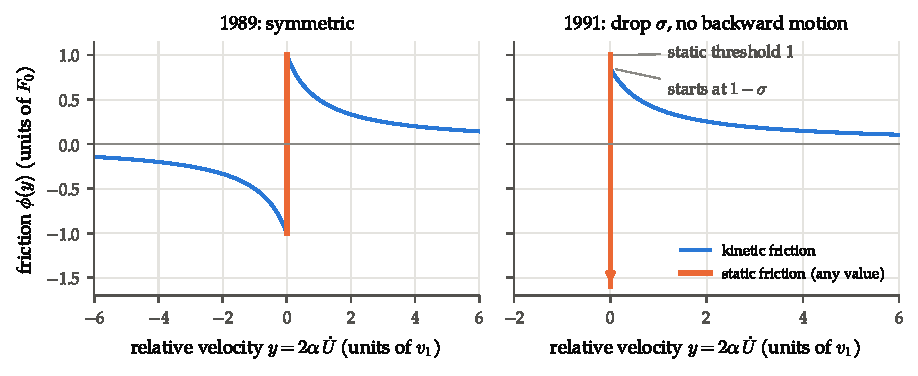
\includegraphics[width=\linewidth]{bk/friction.pdf}
  \caption{The friction laws of Carlson and Langer (1989, left) and of Carlson, Langer, Shaw and Tang (1991, right,
  drawn with $\sigma=0.15$ for visibility; the papers use $\sigma=0.01$). The vertical orange segments show the range of
  values that static friction can take at zero velocity.}
  \label{fig:friction}
\end{figure}

% ======================================================================
\section{Simple motions}
\label{sec:bk-simple}

\subsection{A single block: periodic stick--slip}

Consider first one block with no neighbours (or, equivalently, the whole chain moving rigidly). Its equation is
$\ddot U = (\nu\tau - U) - \phi(2\alpha\dot U)$. While it is stuck, the spring force $\nu\tau - U$ grows linearly with time.
When it reaches 1, the block slips.

If $\alpha$ is large, friction becomes small almost immediately, and the motion is approximately that of a free harmonic
oscillator, $\ddot U \approx \nu\tau - U$. Starting from the slip point, where $\nu\tau - U = 1$, and neglecting the plate
motion during the short slip, the solution is $U(\tau) = U_{\text{slip}} + 1 - \cos(\tau-\tau_{\text{slip}})$. The block
moves forward by 2 (in units of $D_0$) in a time $\pi$ and stops when its velocity vanishes; the spring force is then $-1$,
within the range of static friction, so the block sticks. The plate needs a time $2/\nu$ to load the spring again from
$-1$ to $+1$, and the cycle repeats. For smaller $\alpha$ friction removes part of the energy, and the slip is shorter.
\Cref{fig:single-block} shows the cycle computed numerically with the 1991 law for $\alpha=2.5$ and $\alpha=0.5$.

\begin{figure}[t]
  \centering
  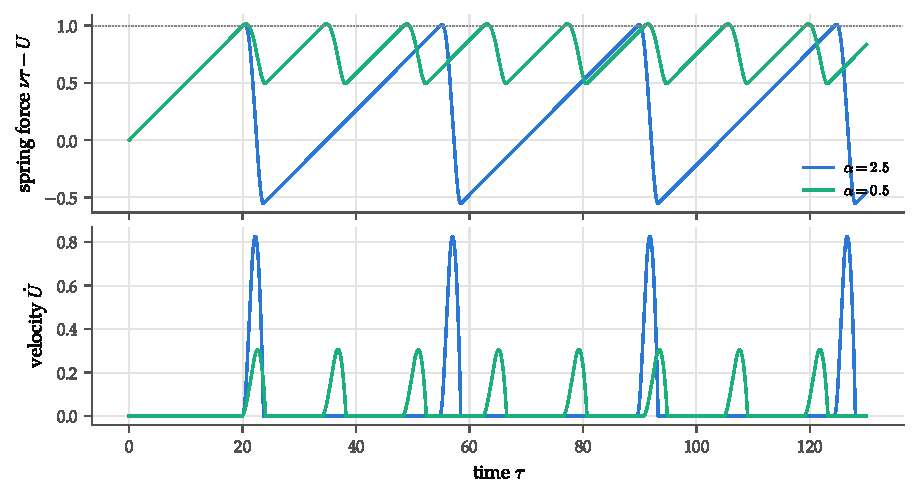
\includegraphics[width=\linewidth]{bk/single_block.pdf}
  \caption{Periodic stick--slip of a single block ($\nu=0.05$, $\sigma=0.05$). Top: spring force; the block slips each time it
  reaches the threshold 1 (dotted). Bottom: velocity. With strong velocity weakening ($\alpha=2.5$) each slip releases most of
  the stored force; with weak weakening ($\alpha=0.5$) only a small part.}
  \label{fig:single-block}
\end{figure}

\subsection{One block slipping inside a stuck chain}
\label{sec:one-block-event}

Now consider block $j$ in a chain whose other blocks are stuck, at the moment its spring force reaches the threshold.
Just before the slip, the forces on it balance exactly: spring force $= 1 =$ static friction. Let $\delta U$ be its
displacement after the slip starts.
\begin{enumerate}
  \item Moving block $j$ by $\delta U$ while its neighbours stay fixed stretches the two coupling springs and the pulling
    spring, changing the spring force on it by $-(2\ell^2+1)\,\delta U$. We write $\omega_1^2 = 2\ell^2+1$.
  \item Friction drops from 1 to $1-\sigma$. If $\ell$ is large the block moves slowly (see below) and the velocity
    dependence of $\phi$ can be neglected, so friction stays at about $1-\sigma$.
  \item The net force is therefore $1 - \omega_1^2\delta U - (1-\sigma) = \sigma - \omega_1^2\delta U$, and
    \begin{equation}
      \delta\ddot U = \sigma - \omega_1^2\,\delta U,\qquad \delta U(0)=\delta\dot U(0)=0 .
    \end{equation}
  \item The solution is a half oscillation about the new equilibrium $\sigma/\omega_1^2$:
    \begin{equation}
      \delta U(\tau) = \frac{\sigma}{\omega_1^2}\bigl(1-\cos\omega_1\tau\bigr).
      \label{eq:one-block}
    \end{equation}
    The velocity $\delta\dot U = (\sigma/\omega_1)\sin\omega_1\tau$ returns to zero at $\tau = \pi/\omega_1$. The block has then
    moved by
    \begin{equation}
      \delta U_1 = \frac{2\sigma}{\omega_1^2} = \frac{2\sigma}{2\ell^2+1}.
      \label{eq:dU1}
    \end{equation}
    At that moment the net force on it is $\sigma - 2\sigma = -\sigma$, which static friction can hold, so it sticks.
\end{enumerate}
The largest velocity, $\sigma/\omega_1$, is small when $\ell$ is large, which is the justification Carlson \emph{et al.} give for step 2.
The \emph{moment} of this event, the product of the block spacing and the displacement, is then
\begin{equation}
  M_1 = a\,\delta U_1 = \frac{2\sigma a}{2\ell^2+1} \approx \frac{\sigma a}{\ell^2}.
  \label{eq:M1}
\end{equation}
For $\ell = 6$ and $\sigma = 0.01$, $M_1\approx 2.7\times10^{-4}\,a$. This is the smallest possible event of the model and
sets the lower end of all size distributions.

\paragraph{The effect of velocity weakening.} Step 2 is less innocent than it looks. Although the velocity is small, what matters
is the change of friction it produces, $2\alpha\,\delta\dot U$, compared with the drop $\sigma$, and these are of the same order. Keeping
the linear term of the friction law, $\phi\approx(1-\sigma)-2\alpha\,\delta\dot U$, the equation of motion becomes
\begin{equation}
  \delta\ddot U - 2\alpha\,\delta\dot U + \omega_1^2\,\delta U = \sigma ,
\end{equation}
a harmonic oscillator with \emph{negative} damping. With $\omega = \sqrt{\omega_1^2-\alpha^2}$, its solution starting from rest is
\begin{equation}
  \delta U(\tau) = \frac{\sigma}{\omega_1^2}\left[1 - e^{\alpha\tau}\left(\cos\omega\tau - \frac{\alpha}{\omega}\sin\omega\tau\right)\right],
  \qquad
  \delta\dot U(\tau) = \frac{\sigma}{\omega}\,e^{\alpha\tau}\sin\omega\tau ,
\end{equation}
as can be checked by substitution. The velocity vanishes again at $\tau = \pi/\omega$, where
\begin{equation}
  \delta U_1 = \frac{\sigma}{\omega_1^2}\left(1 + e^{\pi\alpha/\omega}\right).
  \label{eq:dU1-alpha}
\end{equation}
For $\alpha\to0$ this reduces to \cref{eq:dU1}. For $\ell=6$ and $\alpha=3$, however, $\omega = 8$ and the factor
$\tfrac12(1+e^{3\pi/8})\approx2.1$: the one-block slip is about twice the estimate \cref{eq:dU1}. Our simulations (Chapter~6) give
$M_1 = 5.75\times10^{-4}a$ for these parameters, against $5.82\times10^{-4}a$ from \cref{eq:dU1-alpha} (the small remaining difference
comes from the curvature of the friction law) and $2.74\times10^{-4}a$ from \cref{eq:M1}.

\paragraph{Where the released force goes.} Before the slip the spring force on block $j$ was 1; after it, $1-\omega_1^2\delta U_1$.
The block has shed a force $\Delta f = \omega_1^2\,\delta U_1$, equal to $2\sigma$ without velocity weakening and to
$\sigma(1+e^{\pi\alpha/\omega})$ with it. Each neighbour has been pulled forward by its coupling spring with an extra
force $\ell^2\delta U_1$, so the two neighbours together received
\begin{equation}
  2\ell^2\,\delta U_1 = \frac{2\ell^2}{2\ell^2+1}\,\Delta f ,
\end{equation}
a fraction $2\ell^2/(2\ell^2+1)$ of the force shed, whatever the value of $\Delta f$. The remaining fraction,
\begin{equation}
  \epsilon = \frac{1}{2\ell^2+1},
  \label{eq:eps-bk}
\end{equation}
went into the block's own pulling spring and is no longer available to the chain. This is exactly the \emph{toppling} of a
sandpile site with \emph{bulk dissipation} $\epsilon$, discussed in \cref{sec:soc-implications}: a site at threshold releases
an amount of ``stress'', most of which goes to its neighbours and a small part of which is lost. A neighbour that was within
$\ell^2\delta U_1\approx\Delta f/2$ of its own threshold is pushed over it and slips in turn. This observation is the starting point
of the mapping in Chapter~5.

\subsection{Several blocks slipping together}

Carlson and Langer also consider $n$ neighbouring blocks that are all at threshold and slip together as a rigid group. The
coupling springs inside the group are not stretched when all of them move by the same amount; only the two springs at the
ends of the group and the $n$ pulling springs resist the motion. Per block, a common displacement $\delta$ therefore changes the
spring force by $-(1 + 2\ell^2/n)\,\delta$. Repeating the steps above with $\omega_1^2$ replaced by
\begin{equation}
  \Omega_n^2 = 1 + \frac{2\ell^2}{n},
\end{equation}
each block of the group moves by $\delta_n = 2\sigma/\Omega_n^2$, and the moment of the event is
\begin{equation}
  M_n = n\,a\,\delta_n = \frac{2\sigma a\,n^2}{n+2\ell^2}.
  \label{eq:Mn}
\end{equation}
For $n=1$ this is \cref{eq:M1}. For small groups, $n\ll\ell^2$, $M_n\approx \sigma a n^2/\ell^2$, so the moments of the smallest
events come in a discrete sequence $M_1, 4M_1, 9M_1,\dots$; they appear as separate peaks at the small-moment end of the
distributions. (The 1989 paper derives an analogous sequence for its friction law, in which the size of the few-block events is set by the
loading speed $\nu$ instead of $\sigma$; the corresponding peaks are clearly visible in its Fig.~6.) For $n\gg\ell^2$, $M_n\approx2\sigma a n$.

% ======================================================================
\section{Uniform sliding is unstable}
\label{sec:bk-instability}

A possible motion of the chain is steady sliding: all blocks move together with the plate, at the plate speed, with the
pulling springs stretched just enough to balance friction. In the frame of \cref{eq:bk-CL} this is $U^{\text{CL}}_0 =
-\phi(2\alpha\nu)$, a constant. Is this motion stable? To find out, add a small wavy perturbation,
\begin{equation}
  U^{\text{CL}}(s,\tau) = U^{\text{CL}}_0 + u\,e^{iqs+\Omega\tau},
\end{equation}
with wave number $q$ and growth rate $\Omega$, and insert it into the continuum form of \cref{eq:bk-CL}.
\begin{enumerate}
  \item Expand friction to first order in the small velocity $\dot u$: $\phi(2\alpha\nu + 2\alpha\dot u)\approx\phi(2\alpha\nu) +
    2\alpha\phi'(2\alpha\nu)\,\dot u$. The constant term balances $U^{\text{CL}}_0$. Define $\bar\alpha = -\alpha\,\phi'(2\alpha\nu)$,
    which is positive because friction \emph{decreases} with velocity; for small $\nu$, $\phi'\approx-1$ and $\bar\alpha\approx\alpha$.
  \item The remaining linear terms give $\Omega^2 u = -\xi^2q^2 u - u + 2\bar\alpha\,\Omega u$, i.e.
    \begin{equation}
      \Omega^2 - 2\bar\alpha\,\Omega + (1+\xi^2q^2) = 0 .
    \end{equation}
  \item The solutions are
    \begin{equation}
      \Omega(q) = \bar\alpha \pm\sqrt{\bar\alpha^2 - 1 - \xi^2q^2}.
      \label{eq:dispersion}
    \end{equation}
\end{enumerate}
For every $q$ the real part of $\Omega$ (with the $+$ sign) is at least $\bar\alpha>0$ (\cref{fig:dispersion}): perturbations of
\emph{every} wavelength grow. Steady sliding is unstable.

The physical reason is visible in the equation: the term $+2\bar\alpha\,\Omega u$ is a \emph{negative damping}. Ordinary friction,
which increases with velocity, damps oscillations. Velocity-weakening friction does the opposite: a block that moves a little faster
than its neighbours feels less friction and accelerates further, so any irregularity grows. This instability is the source of the
complex, chaotic behaviour of the BK model, which contains no randomness at all.

\begin{figure}[t]
  \centering
  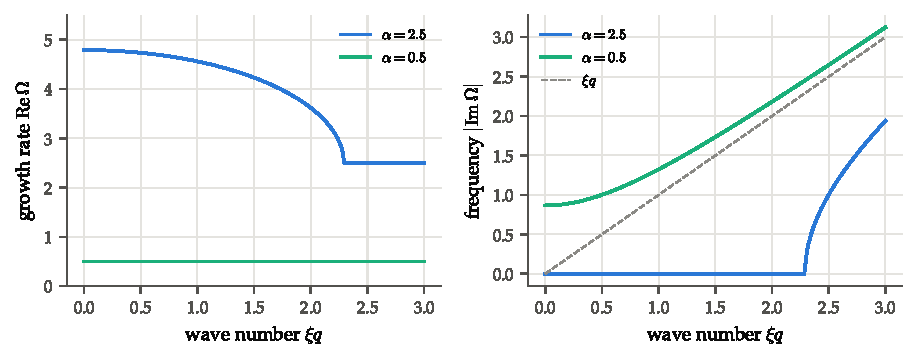
\includegraphics[width=\linewidth]{bk/dispersion.pdf}
  \caption{Linear stability of uniform sliding, \cref{eq:dispersion}. Left: growth rate of a perturbation of wave number $q$; it is
  positive for every $q$. Right: oscillation frequency; for $\xi q\gg\bar\alpha$ it approaches $\xi q$, i.e.\ short perturbations travel
  as waves with speed $\xi$.}
  \label{fig:dispersion}
\end{figure}

% ======================================================================
\section{Growing slip pulses}
\label{sec:bk-pulses}

The same instability acts during a slipping event, and Carlson and Langer use it to understand how events grow. Consider a region of
the fault in which all blocks are just at the threshold of slipping. In the continuum limit with $\nu\to0$, such a state $U_c(s)$
satisfies the force balance with friction at its maximum,
\begin{equation}
  \xi^2\,\frac{\dd^2U_c}{\dd s^2} - U_c = 1 \qquad\Longrightarrow\qquad U_c(s) = -1 + \epsilon\cosh(s/\xi)
\end{equation}
(in the frame of \cref{eq:bk-CL}), where the small constant $\epsilon$ measures how far the region is from being exactly at threshold.

Suppose a small slip starts at a point $s_0$ of this region, and write $U = U_c + \delta U$. In the slipping region friction is
$\phi\approx(1-\sigma) - 2\alpha\,\delta\dot U$ (the drop $\sigma$ plus the linear decrease with slope $-1$). Inserting this,
\begin{equation}
  \delta\ddot U = \xi^2\,\delta U'' - \delta U + \sigma + 2\alpha\,\delta\dot U .
\end{equation}
Differentiate once with respect to time to obtain an equation for the slip velocity $w = \delta\dot U$; the constant $\sigma$ drops out:
\begin{equation}
  \ddot w = \xi^2 w'' - w + 2\alpha\,\dot w .
  \label{eq:telegraph}
\end{equation}
This is a wave equation with negative damping. To solve it, separate the growth: write $w = e^{\alpha\tau}\,W$. Then
$\dot w = e^{\alpha\tau}(\alpha W + \dot W)$ and $\ddot w = e^{\alpha\tau}(\alpha^2W + 2\alpha\dot W + \ddot W)$. Substituting and
cancelling $e^{\alpha\tau}$,
\begin{equation}
  \alpha^2W + 2\alpha\dot W + \ddot W = \xi^2W'' - W + 2\alpha^2W + 2\alpha\dot W
  \quad\Longrightarrow\quad
  \ddot W = \xi^2W'' + (\alpha^2-1)\,W .
\end{equation}
For a pulse much narrower than $\xi/\sqrt{|\alpha^2-1|}$, the second derivative $W''$ is much larger than the last term, which can be
neglected. What remains is the ordinary wave equation, whose solution (d'Alembert) is two copies of the initial pulse travelling in
opposite directions with speed $\xi$. Restoring the factor $e^{\alpha\tau}$, a narrow kick at $s_0$ develops into
\begin{equation}
  \delta\dot U(s,\tau) \approx \frac{w_0}{2}\,e^{\alpha\tau}\Bigl[\delta(s-s_0-\xi\tau) + \delta(s-s_0+\xi\tau)\Bigr]:
  \label{eq:pulses}
\end{equation}
\emph{two pulses that run outward at the sound speed $\xi$ and grow exponentially at the rate $\alpha$}. Carlson \emph{et al.} take the
initial kick to be a one-block event, with $w_0 = \sigma\xi/\omega_1^2$.

\Cref{fig:pulses} shows this mechanism in the discrete chain: a numerical solution of the linearised equations of motion, started from a
short velocity kick a few blocks wide. Two pulses run outward at $\ell$ blocks per unit time and grow roughly as $e^{\alpha\tau}$. The
linear equations allow negative velocities, which the real model forbids; the linear picture is therefore valid only for the early,
small-amplitude stage of an event.

\begin{figure}[t]
  \centering
  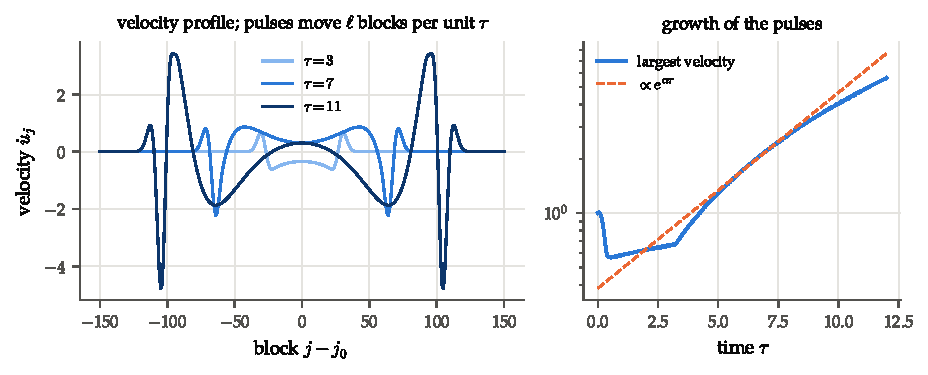
\includegraphics[width=\linewidth]{bk/pulses.pdf}
  \caption{Growing slip pulses in the linearised chain ($\ell=10$, $\alpha=0.25$, 301 blocks), started from a short velocity kick at the
  centre. Left: velocity profile at three times. Right: the largest velocity in the chain against time, compared with $e^{\alpha\tau}$.}
  \label{fig:pulses}
\end{figure}

% ======================================================================
\section{The localization length}
\label{sec:bk-localization}

The growing pulses explain why there are two kinds of large events. Suppose the region that is close to threshold, the
\emph{triggering zone}, has length $\Delta s$, and the event starts near its middle. Each pulse travels a distance $\Delta s/2$ before it
reaches the edge of the zone, which takes a time $\Delta\tau=\Delta s/(2\xi)$. Beyond the edge, the blocks are more firmly stuck. If the pulse
is still small when it gets there, it cannot push these blocks over their threshold and dies out: the event stays \emph{localized} inside
the zone. If the pulse has grown large, it breaks through and keeps going: the event becomes \emph{delocalized}.

\paragraph{The localization condition.} The displacement that a pulse produces at a point at distance $r$ from $s_0$ is the time integral
of the slip velocity there. Since $\int\delta(s_0 + r - s_0 - \xi\tau)\,\dd\tau = 1/\xi$, \cref{eq:pulses} gives
\begin{equation}
  \delta U(r) = \frac{w_0}{2\xi}\,e^{\alpha r/\xi} = \frac{\sigma}{2\omega_1^2}\,e^{\alpha r/\xi}.
\end{equation}
Carlson \emph{et al.} require that this displacement be smaller than a number of order one at the edge of the zone, $r=\Delta s/2$. With
$2\omega_1^2\approx4\ell^2$, the condition $\delta U(\Delta s/2) < 1$ reads
\begin{equation}
  \frac{\sigma}{4\ell^2}\,e^{\alpha\Delta s/(2\xi)} < 1
  \quad\Longleftrightarrow\quad
  \Delta s < \tilde\xi \equiv \frac{2\xi}{\alpha}\,\ln\frac{4\ell^2}{\sigma} .
  \label{eq:xi-tilde}
\end{equation}
Events in zones shorter than $\tilde\xi$ stay localized; longer ones run away. The \emph{localization length} $\tilde\xi$ plays the role of
a correlation length: it is the size of the largest ``ordinary'' event.

\paragraph{The crossover moment.} The total moment of a marginally localized event is the integral of the slip velocity over space and
time. Integrating \cref{eq:pulses} over $s$ gives $w_0e^{\alpha\tau}$, and integrating this over the duration $\Delta\tau = \tilde\xi/(2\xi)$,
\begin{equation}
  \tilde M = \int_0^{\Delta\tau} w_0\,e^{\alpha\tau}\,\dd\tau = \frac{w_0}{\alpha}\left(e^{\alpha\Delta\tau}-1\right)
  \approx \frac{\sigma\xi}{2\ell^2\alpha}\cdot\frac{4\ell^2}{\sigma} = \frac{2\xi}{\alpha},
  \label{eq:M-tilde}
\end{equation}
using $e^{\alpha\Delta\tau} = 4\ell^2/\sigma\gg1$ from \cref{eq:xi-tilde}. Remarkably, $\tilde M$ does not depend on $\sigma$: a smaller
$\sigma$ means a weaker initial kick, which must grow for longer, but the final moment is the same. Carlson \emph{et al.} stress that these
estimates set only the \emph{scales}; the numerical prefactors are not reliable.

\paragraph{The 1989 version.} In the 1989 paper the kick is set by the loading speed $\nu$ instead of $\sigma$, and the localization criterion is
that the displacement at the edge be smaller than $\ell^{-2}$ (the displacement needed to push a neighbour over threshold through one coupling
spring), giving~\cite{CarlsonLanger1989}
\begin{equation}
  \tilde\xi_{1989} \approx \frac{2\xi}{\alpha}\,\ln\frac{4\xi}{\nu a},\qquad \tilde M \approx\frac{2\xi}{\alpha}.
\end{equation}
For their main parameters ($\ell=10$, $\alpha=2.5$, $\nu=0.01$) this gives $\tilde\xi\approx66\,a$, compared with system sizes $N=100$--$400$.

\paragraph{The critical parameter.} In both versions $\tilde\xi$ grows logarithmically without bound as the triggering parameter goes to zero
($\sigma\to0$ in 1991, $\nu\to0$ in 1989). This parameter therefore plays the role of the distance from a critical point: only in the limit
$\sigma\to0$ does the range of localized events become infinite. The logarithmic dependence means, however, that this limit is approached very
slowly (\cref{fig:localization}). For the parameters of the 1991 paper ($\alpha=3$, $\sigma=0.01$) the localization length is about 38 blocks for
$\ell=6$ and 88 blocks for $\ell=12$, while the smallest and crossover moments are $M_1\approx2.7\times10^{-4}a$ and $\tilde M=4a$ for $\ell=6$: the
localized events span about four decades in moment.

\begin{figure}[t]
  \centering
  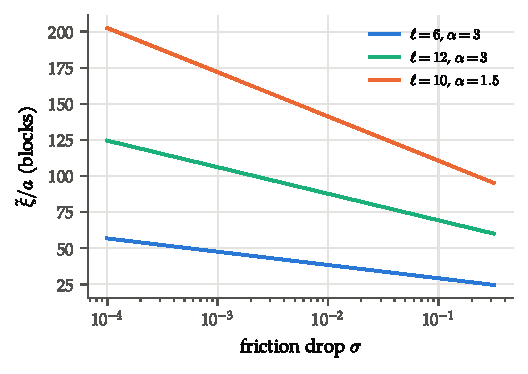
\includegraphics[width=0.55\linewidth]{bk/localization.pdf}
  \caption{Localization length \cref{eq:xi-tilde}, in units of the block spacing, as a function of the friction drop $\sigma$.}
  \label{fig:localization}
\end{figure}

% ======================================================================
\section{Three kinds of events and the cycle of the fault}
\label{sec:bk-events}

Carlson and Langer found that the events of the model fall into three classes, each with its own physics:
\begin{enumerate}
  \item \textbf{Microscopic events}, involving one or a few blocks (\cref{sec:one-block-event}). Their moments are of order $M_1 = 2\sigma a/(2\ell^2+1)$
    and come in discrete steps (\cref{eq:Mn}). They release very little stress and mainly smooth the configuration on the scale of a few blocks.
  \item \textbf{Localized events}, larger than microscopic but smaller than the localization length, with moments up to about $\tilde M = 2\xi/\alpha$.
    These form the broad, power-law ``scaling region'' of the size distribution.
  \item \textbf{Delocalized events}, in which the pulses break out of the triggering zone. They propagate along the fault at the sound speed, can
    involve hundreds or thousands of blocks, and displace them by amounts of order one. They are much more frequent than an extrapolation of the
    scaling region would predict.
\end{enumerate}

The 1991 paper describes how the classes are related (its Fig.~2, which shows a sequence of stuck configurations). After a large delocalized event the
configuration is rough on all scales below $\tilde\xi$, because the instability of \cref{sec:bk-instability} amplifies irregularities while the blocks slip.
The many small and localized events that follow do not move the fault much; their main effect is to \emph{smooth} the configuration: a group of blocks that
lags behind its neighbours slips and catches up. Once a region of size about $\tilde\xi$ has become smooth enough and reaches the threshold, it triggers the
next delocalized event, which roughens the configuration again. In this picture the localized events are not an independent self-organized critical
process: their statistics are controlled by the delocalized events, which set up the rough configurations that the small events then smooth out.

% ======================================================================
\section{Statistics of events}
\label{sec:bk-stats}

\subsection{Definitions}

The \emph{moment} of an event is the total slip it produces, in units of $D_0$ times the block spacing:
\begin{equation}
  M = a\sum_{j}\delta U_j ,
\end{equation}
where $\delta U_j$ is the displacement of block $j$ during the event and the sum runs over the blocks that moved. Its magnitude is $\mu = \ln M$
(Chapter~\ref{ch:intro}). Carlson and Langer use $a=1$, so $M$ is the sum of the block displacements.

In the 1989 paper, with a finite loading speed, the distribution of events is described by $\mathcal R(\mu)$, the number of events \emph{per unit time
and per unit length} of the fault with magnitude between $\mu$ and $\mu+\dd\mu$. In the limit $\nu\to0$ of the 1991 paper, time has no meaning between events,
and the natural quantity is the number of events \emph{per unit plate displacement} and per unit length,
\begin{equation}
  \mathcal D(\mu) = \frac{\mathcal R(\mu)}{\nu}.
\end{equation}

\paragraph{The sum rule.} Over a long time $T$ the plate moves by $\nu T$, and every block must on average move by the same amount (otherwise its pulling
spring would stretch without limit). The total moment of all events in time $T$ on a fault of length $L$ is therefore $L\,\nu T$. Since the number of events
in $\dd\mu$ is $\mathcal R(\mu)\,\dd\mu\, L T$, each with moment $e^\mu = M$,
\begin{equation}
  \int M\,\mathcal R(\mu)\,\dd\mu = \nu,\qquad\text{equivalently}\qquad \int M\,\mathcal D(\mu)\,\dd\mu = 1 .
  \label{eq:sumrule}
\end{equation}
This exact constraint links the frequencies of small and large events: if the small events do not move the fault forward enough, large events must do it.

\subsection{The 1989 results}

Carlson and Langer simulated chains of $N=100$ to $400$ blocks with $\ell=10$, $\nu=0.01$ and $0.001$, and $\alpha$ from 1 to 4, over $40$ to $1000$ loading
periods $2/\nu$. Their distributions $\ln\mathcal R(\mu)$ show:
\begin{itemize}[nosep]
  \item at small $\mu$, sharp peaks from the one-block and few-block microscopic events;
  \item in the middle, a straight ``scaling region'' $\mathcal R\propto e^{-b\mu}$ with $b\approx1$ for $\alpha\gtrsim2.5$; for smaller $\alpha$ the slope is
    flatter ($b\approx0.35$ at $\alpha=1$);
  \item at large $\mu$, a bump of delocalized ``great'' events, near the largest possible moment $\mu_L=\ln(2N)$ (all blocks displaced by 2).
\end{itemize}
They explained the scaling region with a dimensional argument. In the continuum equation \cref{eq:bk-cont} the only length is $\xi$, so if neither $a$ nor
$N$ matters in the scaling region, $\mathcal R$ can depend on $M$ only through $M/\tilde M = \alpha M/2\xi$:
\begin{equation}
  \mathcal R_S(\mu) = \frac{\nu}{M}\,\mathcal C\!\left(\frac{\alpha M}{2\xi},\alpha\right)
  \;\approx\; \frac{\nu}{M}\,\mathcal C_0(\alpha)\left(\frac{\alpha M}{2\xi}\right)^{\eta}\qquad (M\ll\tilde M).
\end{equation}
Comparing with $\mathcal R\propto e^{-b\mu} = M^{-b}$ gives $b = 1-\eta$; $b=1$ corresponds to $\eta=0$, a power law with no ``anomalous dimension''. In the language
of Chapter~\ref{ch:intro}, $b = 1$ means a moment density $P(M)\propto M^{-2}$, $\tau=2$.

The authors note several limitations of their data. The great events appear roughly once per loading period, and the runs covered between 40 and 1000 loading
periods, so the large-event part of the distribution rests on relatively few events. The system sizes were only a few times the localization length
($\tilde\xi\approx66$ for $N=100$), and they observed that the distributions depend on $N$ near the upper end. Finally, the finite loading speed introduces
another length, $2\xi/\nu$, the distance a sound wave travels in one loading period; for $\nu=0.01$ and large $N$ they found resonant propagating modes in which
the picture of separate events breaks down.

\subsection{The 1991 results}

With the $\sigma$ friction law and $\nu\to0$, Carlson, Langer, Shaw and Tang simulated much longer chains: $N=4096$ and $8192$, with $\alpha=3$, $\sigma=0.01$ and
$\ell=6$, 8 and 12 (their Fig.~3), so that even the largest events never span the whole system. Their main findings are:
\begin{itemize}
  \item The distribution $\mathcal D(\mu)$ has a scaling region of localized events with slope $b\approx0.92$ (from a least-squares fit), a pronounced minimum
    just below $M=\tilde M$, and a peak of delocalized events. The minima for different $\ell$ coincide when plotted against $\ln(M/\xi)$, confirming that the
    crossover is at $M\approx\tilde M\propto\xi$.
  \item They summarise the distribution as
    \begin{equation}
      \mathcal D(\mu)\approx
      \begin{cases}
        A\,(\tilde M/M)^{b}, & M_1<M<\tilde M,\\
        A'\,(M/M^*)^{-b'}, & \tilde M<M<M^*,\\
        0, & M<M_1\ \text{or}\ M>M^*,
      \end{cases}
      \label{eq:D91}
    \end{equation}
    with $b\approx1$ and $b'\approx-1$: the delocalized events \emph{rise} with $M$ up to a sharp upper cutoff $M^*$.
  \item The upper cutoff grows with $\ell$ faster than $\tilde M$, roughly as $M^*/\tilde M\propto\ell$ for large $\alpha$. Because the ratio depends on
    $\ell=\xi/a$ and not only on $\xi$, the block spacing $a$ (the ``ultraviolet cutoff'') matters: the model has no simple continuum limit.
  \item For small $\alpha$ ($\alpha=1$, $\sigma=0.01$, $\ell=6$, 10, 14) the separation between localized and delocalized events disappears, and the whole
    distribution is a single power law with $b\approx0.35$.
  \item The localization length measured from the distribution of the number of blocks per event is of the order of $\tilde\xi$ but typically larger than
    \cref{eq:xi-tilde}.
\end{itemize}
Translated into the moment density $P(M)$ (\cref{eq:CL-b-tau}), $b\approx1$ in the localized region means $\tau\approx2$, $b'\approx-1$ for the delocalized events
means $P(M)\approx$ constant up to $M^*$, and $b\approx0.35$ at $\alpha=1$ means $\tau\approx1.35$.

% ======================================================================
\section{Why the two papers differ}
\label{sec:bk-differences}

\Cref{tab:89vs91} collects the differences between the two studies. They are not two runs of the same model with more or less data: they are different models,
analysed in different limits, with different observables. A simulation that mixes features of both, for example the friction drop of 1991 with a finite loading
speed and the event definition of 1989, cannot be expected to reproduce either. Even within one model, the 1989 runs were short and the systems small compared
with the length scales involved, which makes the delocalized part of the distribution and the shape near the crossover statistically fragile.

\begin{table}[t]
\centering
\caption{The two studies of the BK model by Carlson and collaborators.}
\label{tab:89vs91}
\begin{tabular}{@{}lp{55mm}p{55mm}@{}}
\toprule
 & 1989~\cite{CarlsonLanger1989} & 1991~\cite{Carlson1991} \\
\midrule
friction at rest & $[-1,1]$; backward slip possible & $(-\infty,1]$; no backward slip \\
onset of slip & smooth, friction starts at 1 & abrupt drop to $1-\sigma$ \\
loading speed & finite, $\nu = 0.01$, $0.001$ & $\nu\to0$ (event-driven) \\
critical parameter & $\nu$ & $\sigma$ \\
localization length & $\frac{2\xi}{\alpha}\ln\frac{4\xi}{\nu a}$ & $\frac{2\xi}{\alpha}\ln\frac{4\ell^2}{\sigma}$ \\
distribution & $\mathcal R(\mu)$ per unit time & $\mathcal D(\mu)=\mathcal R/\nu$ per unit displacement \\
system size & $N = 100$--$400$ & $N = 4096$--$8192$ \\
stiffness & $\ell = 10$ & $\ell = 6$, 8, 12 (and 3, 10, 14) \\
duration of runs & 40--1000 loading periods & hundreds to thousands of loading periods \\
\bottomrule
\end{tabular}
\end{table}

For this thesis we therefore take the 1991 model as the reference: its definition is cleaner (no dependence on $\nu$), its simulations are larger, and it is the one
that maps most naturally onto a sandpile, where grains are also added only when all activity has stopped. The 1989 model with finite $\nu$ is treated afterwards, as a
variation.

% ======================================================================
\section{Summary: what a sandpile would have to capture}
\label{sec:bk-summary}

The analysis of this chapter identifies the ingredients that determine the statistics of the BK model:
\begin{enumerate}
  \item \textbf{A threshold with a drop.} A block slips when its spring force reaches the static threshold, and then sheds a force $\Delta f$ of order $\sigma$ (\cref{sec:one-block-event}).
    This is the analogue of a sandpile site toppling when its height reaches the critical value.
  \item \textbf{Redistribution with bulk dissipation.} Of the force shed, a fraction $2\ell^2/(2\ell^2+1)$ goes to the two neighbours and a fraction
    $\epsilon = 1/(2\ell^2+1)$ is lost into the pulling spring. In sandpile language this is a toppling rule with bulk dissipation $\epsilon$, which introduces a length
    of order $\ell$, the stiffness length.
  \item \textbf{Uniform, deterministic driving.} The plate loads all blocks at the same rate, and in the limit $\nu\to0$ it is moved only between events, exactly like a
    sandpile that is driven only when it is stable.
  \item \textbf{Inertia and velocity weakening.} Slipping blocks have velocities, and velocity-weakening friction amplifies slip pulses at the rate $\alpha$
    (\cref{sec:bk-pulses}). This is what produces the delocalized events and the localization length $\tilde\xi\propto(\xi/\alpha)\ln(4\ell^2/\sigma)$. A sandpile, whose
    topplings have no memory of velocity, has no counterpart of this ingredient.
\end{enumerate}
The first three ingredients define a sandpile model of the Olami--Feder--Christensen type. Chapter~5 derives this model from \cref{eq:bk} and asks how much of the BK
statistics survives when the fourth ingredient, inertia, is removed. The answer to that question is the central result of this thesis.

\chapter{From the Burridge--Knopoff model to a sandpile}
\label{ch:mapping}

\newcommand{\mapSandDistEnd}{1.0e-12}
\newcommand{\mapLyapPlate}{47}
\newcommand{\mapperFixed}{25{,}376}
\newcommand{\mapperPlateFixed}{0.04248}
\newcommand{\mapperTopplingsFixed}{73.0}
\newcommand{\mapperReset}{152}
\newcommand{\mapperPlateReset}{0.07565}
\newcommand{\mapperTopplingsReset}{130.0}
\newcommand{\mapdropAthreeLsix}{0.04248}
\newcommand{\mapnoiseMaxfixedsix}{125}
\newcommand{\mapnoiseMeanfixedsix}{8.7}
\newcommand{\mapnoiseMaxMfixedsix}{0.24}
\newcommand{\mapnoiseMaxresetsix}{132}
\newcommand{\mapnoiseMeanresetsix}{8.3}
\newcommand{\mapnoiseMaxMresetsix}{0.40}
\newcommand{\mapnoiseMaxfixedtwelve}{247}
\newcommand{\mapnoiseMeanfixedtwelve}{15.0}
\newcommand{\mapnoiseMaxMfixedtwelve}{0.12}
\newcommand{\mapnoiseMaxresettwelve}{267}
\newcommand{\mapnoiseMeanresettwelve}{14.3}
\newcommand{\mapnoiseMaxMresettwelve}{0.20}
\newcommand{\mapbkaBlBAevents}{8{,}600{,}000}
\newcommand{\mapbkaBlBAmaxblocks}{2971}
\newcommand{\mapbkaBlBAplate}{501}
\newcommand{\mapbkaBlBEevents}{7{,}800{,}000}
\newcommand{\mapbkaBlBEmaxblocks}{6769}
\newcommand{\mapbkaBlBEplate}{511}
\newcommand{\mapbkaBlGevents}{5{,}600{,}000}
\newcommand{\mapbkaBlGmaxblocks}{1500}
\newcommand{\mapbkaBlGplate}{517}
\newcommand{\mapbkaDlBCevents}{5{,}000{,}000}
\newcommand{\mapbkaDlBCmaxblocks}{7359}
\newcommand{\mapbkaDlBCplate}{1018}
\newcommand{\mapbkaDlGevents}{3{,}000{,}000}
\newcommand{\mapbkaDlGmaxblocks}{2550}
\newcommand{\mapbkaDlGplate}{1048}
\newcommand{\mapbkaDlIevents}{3{,}000{,}000}
\newcommand{\mapbkaDlImaxblocks}{3178}
\newcommand{\mapbkaDlIplate}{1033}
\newcommand{\mapfixedaBlBAevents}{1{,}099{,}800{,}000}
\newcommand{\mapfixedaBlBAmaxblocks}{121}
\newcommand{\mapfixedaBlBAplate}{300}
\newcommand{\mapfixedaBlGevents}{305{,}200{,}000}
\newcommand{\mapfixedaBlGmaxblocks}{42}
\newcommand{\mapfixedaBlGplate}{300}
\newcommand{\mapfixedaDlBCevents}{1{,}078{,}200{,}000}
\newcommand{\mapfixedaDlBCmaxblocks}{87}
\newcommand{\mapfixedaDlBCplate}{300}
\newcommand{\mapfixedaDlGevents}{172{,}600{,}000}
\newcommand{\mapfixedaDlGmaxblocks}{69}
\newcommand{\mapfixedaDlGplate}{300}
\newcommand{\mapfixedaDlIevents}{276{,}200{,}000}
\newcommand{\mapfixedaDlImaxblocks}{65}
\newcommand{\mapfixedaDlIplate}{300}
\newcommand{\mapnoisefixedwApABlBCevents}{292{,}000{,}000}
\newcommand{\mapnoisefixedwApABlBCmaxblocks}{266}
\newcommand{\mapnoisefixedwApABlBCplate}{300}
\newcommand{\mapnoisefixedwApABlGevents}{89{,}400{,}000}
\newcommand{\mapnoisefixedwApABlGmaxblocks}{138}
\newcommand{\mapnoisefixedwApABlGplate}{300}
\newcommand{\mapnoisefixedwApAFlBCevents}{166{,}000{,}000}
\newcommand{\mapnoisefixedwApAFlBCmaxblocks}{265}
\newcommand{\mapnoisefixedwApAFlBCplate}{300}
\newcommand{\mapnoisefixedwApAFlGevents}{60{,}000{,}000}
\newcommand{\mapnoisefixedwApAFlGmaxblocks}{130}
\newcommand{\mapnoisefixedwApAFlGplate}{301}
\newcommand{\mapnoisefixedwApClBCevents}{80{,}400{,}000}
\newcommand{\mapnoisefixedwApClBCmaxblocks}{247}
\newcommand{\mapnoisefixedwApClBCplate}{300}
\newcommand{\mapnoisefixedwApClGevents}{30{,}000{,}000}
\newcommand{\mapnoisefixedwApClGmaxblocks}{125}
\newcommand{\mapnoisefixedwApClGplate}{301}
\newcommand{\mapnoiseresetwApABlBCevents}{117{,}800{,}000}
\newcommand{\mapnoiseresetwApABlBCmaxblocks}{413}
\newcommand{\mapnoiseresetwApABlBCplate}{300}
\newcommand{\mapnoiseresetwApABlGevents}{50{,}200{,}000}
\newcommand{\mapnoiseresetwApABlGmaxblocks}{991}
\newcommand{\mapnoiseresetwApABlGplate}{301}
\newcommand{\mapnoiseresetwApAFlBCevents}{138{,}400{,}000}
\newcommand{\mapnoiseresetwApAFlBCmaxblocks}{276}
\newcommand{\mapnoiseresetwApAFlBCplate}{300}
\newcommand{\mapnoiseresetwApAFlGevents}{49{,}000{,}000}
\newcommand{\mapnoiseresetwApAFlGmaxblocks}{137}
\newcommand{\mapnoiseresetwApAFlGplate}{300}
\newcommand{\mapnoiseresetwApClBCevents}{51{,}000{,}000}
\newcommand{\mapnoiseresetwApClBCmaxblocks}{267}
\newcommand{\mapnoiseresetwApClBCplate}{301}
\newcommand{\mapnoiseresetwApClGevents}{22{,}000{,}000}
\newcommand{\mapnoiseresetwApClGmaxblocks}{132}
\newcommand{\mapnoiseresetwApClGplate}{302}
\newcommand{\mapresetaDlBCevents}{3{,}800{,}000}
\newcommand{\mapresetaDlBCmaxblocks}{8191}
\newcommand{\mapresetaDlBCplate}{311}
\newcommand{\mapresetaDlGevents}{600{,}000}
\newcommand{\mapresetaDlGmaxblocks}{4095}
\newcommand{\mapresetaDlGplate}{334}
\newcommand{\mapresetaDlIevents}{1{,}400{,}000}
\newcommand{\mapresetaDlImaxblocks}{4095}
\newcommand{\mapresetaDlIplate}{308}
\newcommand{\maptauAthreeLG}{1.962}
\newcommand{\maperrAthreeLG}{0.006}
\newcommand{\mapbAthreeLG}{0.96}
\newcommand{\maptauAthreeLI}{1.921}
\newcommand{\maperrAthreeLI}{0.004}
\newcommand{\mapbAthreeLI}{0.92}
\newcommand{\maptauAthreeLM}{1.913}
\newcommand{\maperrAthreeLM}{0.002}
\newcommand{\mapbAthreeLM}{0.91}
\newcommand{\maptauAoneLG}{1.400}
\newcommand{\maperrAoneLG}{0.001}
\newcommand{\mapbAoneLG}{0.40}
\newcommand{\maptauAoneLK}{1.363}
\newcommand{\maperrAoneLK}{0.001}
\newcommand{\mapbAoneLK}{0.36}
\newcommand{\maptauAoneLO}{1.357}
\newcommand{\maperrAoneLO}{0.001}
\newcommand{\mapbAoneLO}{0.36}


Chapter~\ref{ch:bk} ended with a list of ingredients that determine the statistics of the Burridge--Knopoff
(BK) model: a threshold with a drop of the force, redistribution of the shed force with partial loss into the
pulling springs, uniform driving, and inertia with velocity weakening. The first three are exactly the
ingredients of a sandpile model. In this chapter we make the correspondence precise: we derive a sandpile model
from the BK equations by removing inertia (\cref{sec:map-derivation}), study its properties
(\cref{sec:map-properties}), and then compare its statistics with those of the full BK model, simulated with the
same parameters (\cref{sec:map-comparison}). The comparison answers the central question of this thesis: which
features of the BK model survive the mapping, and which do not.

% ======================================================================
\section{Derivation}
\label{sec:map-derivation}

\subsection{The force variables}

The natural variable for a sandpile description is not the displacement $U_j$ of a block but the total spring force
acting on it,
\begin{equation}
  f_j = \ell^2\,(U_{j+1}-2U_j+U_{j-1}) + (P - U_j),
  \label{eq:fj}
\end{equation}
with free ends ($U_0\equiv U_1$, $U_{N+1}\equiv U_N$) and $P$ the position of the plate. A stuck block stays stuck as long as
$f_j<1$, and starts to slip when $f_j$ reaches 1: $f_j$ plays the role of the height of a sandpile site, and 1 is the critical
height.

Two properties of $f_j$ follow directly from \cref{eq:fj}.
\begin{enumerate}
  \item \textbf{Response to a slip.} If block $j$ moves forward by $\Delta$ while all other blocks stay where they are, its own
    force changes by $-(2\ell^2+1)\Delta$ (two coupling springs and its pulling spring resist the motion) and the force on each
    neighbour increases by $\ell^2\Delta$ (the coupling spring between them is compressed). For an end block, which has only one
    neighbour, the own force changes by $-(\ell^2+1)\Delta$. We write
    \begin{equation}
      \omega_j^2 = \begin{cases} 2\ell^2+1 & \text{bulk},\\ \ell^2+1 & \text{ends.}\end{cases}
    \end{equation}
  \item \textbf{Total force.} Summing \cref{eq:fj} over all blocks, the coupling terms cancel in pairs (each spring pushes one
    block as much as it pulls the other), so
    \begin{equation}
      \sum_{j=1}^N f_j = N P - \sum_{j=1}^{N} U_j .
      \label{eq:total-force}
    \end{equation}
    This identity is exact, in the full BK model as well. Since the moment of an event is $M = \sum_j\delta U_j$ (with $a=1$), it
    gives the force bookkeeping
    \begin{equation}
      \Delta\Bigl(\sum_j f_j\Bigr) = N\,\Delta P - \sum_{\text{events}} M .
      \label{eq:force-bookkeeping}
    \end{equation}
    The plate adds force $N\,\Delta P$; slip removes exactly as much force as its moment. Because the forces stay bounded, over a long
    time the total moment per block equals the plate displacement: this is the sum rule \cref{eq:sumrule}.
\end{enumerate}

\subsection{The quasi-static approximation}

The BK dynamics is replaced by a sequence of elementary slips under the following assumptions:
\begin{enumerate}[label=(A\arabic*)]
  \item \textbf{One block at a time.} A block that reaches the threshold slips while its neighbours are stuck, as in the one-block
    event of \cref{sec:one-block-event}.
  \item \textbf{A fixed slip.} Each such slip has the size of the one-block event, $\Delta_j = \Delta f/\omega_j^2$, where
    \begin{equation}
      \Delta f = \sigma\left(1+e^{\pi\alpha/\omega}\right),\qquad \omega = \sqrt{2\ell^2+1-\alpha^2},
      \label{eq:map-drop}
    \end{equation}
    is the force shed in a one-block event (\cref{eq:dU1-alpha}).
  \item \textbf{No memory of motion.} After its slip the block is at rest; its neighbours feel only the static change of force
    $\ell^2\Delta_j$. No kinetic energy or momentum is passed on.
  \item \textbf{Slow, uniform driving.} The plate moves only when all blocks are stuck, until the most loaded block reaches the threshold
    (the limit $\nu\to0$).
\end{enumerate}
Under these assumptions the BK model becomes a continuous sandpile on the chain:
\begin{description}[font=\normalfont\itshape]
  \item[Drive.] Raise all $f_j$ by the same amount until $\max_j f_j = 1$.
  \item[Toppling.] A site with $f_j\ge1$ topples: $f_j\to f_j - \Delta f$ and $f_{j\pm1}\to f_{j\pm1} + \ell^2\Delta f/\omega_j^2$. The
    corresponding block has slipped by $\Delta f/\omega_j^2$.
  \item[Avalanche.] Topplings continue until all $f_j<1$. Its moment is the sum of the slips.
\end{description}
\Cref{fig:toppling-map} illustrates the correspondence.

\begin{figure}[t]
\centering
\begin{tikzpicture}[x=10mm,y=10mm,>={Stealth[length=1.8mm]}]
  % plate
  \fill[cblue!12] (-0.3,2.3) rectangle (6.3,2.6); \draw[ink2] (-0.3,2.3) rectangle (6.3,2.6);
  \fill[pattern=north east lines,pattern color=ink2!50] (-0.3,-0.2) rectangle (6.3,0); \draw[ink2] (-0.3,0)--(6.3,0);
  \foreach \x/\c in {0.5/cblue!10,2.5/corange!25,4.5/cblue!10} {
    \draw[ink2,fill=\c] (\x,0) rectangle (\x+1,0.8);
    \draw[ink2,decorate,decoration={zigzag,segment length=2mm,amplitude=0.9mm}] (\x+0.5,0.8)--(\x+0.5,2.3);
  }
  \draw[ink2,decorate,decoration={zigzag,segment length=2mm,amplitude=0.9mm}] (1.5,0.4)--(2.5,0.4);
  \draw[ink2,decorate,decoration={zigzag,segment length=2mm,amplitude=0.9mm}] (3.5,0.4)--(4.5,0.4);
  \draw[->,corange,thick] (3.1,1.0)--(3.9,1.0) node[midway,above,font=\footnotesize] {slip $\Delta$};
  \node[font=\footnotesize,align=center] at (1.0,-0.6) {$+\ell^2\Delta$};
  \node[font=\footnotesize,align=center] at (3.0,-0.6) {$-(2\ell^2{+}1)\Delta$};
  \node[font=\footnotesize,align=center] at (5.0,-0.6) {$+\ell^2\Delta$};
  \node[font=\footnotesize,ink2,anchor=west] at (6.4,-0.6) {change of force $f$};
  \node[font=\footnotesize,ink2,anchor=west] at (6.4,1.6) {pulling spring takes $\Delta$};
  \draw[->,ink2] (6.35,1.6) -- (3.65,1.6);
  \node[font=\footnotesize,ink2,anchor=west] at (6.4,2.45) {plate};
\end{tikzpicture}
\caption{A slip $\Delta$ of one block while its neighbours are stuck, as a sandpile toppling. The block's own force drops by $(2\ell^2+1)\Delta$; each neighbour gains
$\ell^2\Delta$; the remaining $\Delta$ is taken up by the block's pulling spring and is lost to the chain. With $\Delta=\Delta f/(2\ell^2+1)$ the lost fraction of the shed
force is $\epsilon = 1/(2\ell^2+1)$.}
\label{fig:toppling-map}
\end{figure}

Of the force $\Delta f$ shed by a toppling in the bulk, a fraction $2\ell^2/(2\ell^2+1)$ goes to the neighbours, and the fraction
\begin{equation}
  \epsilon = \frac{1}{2\ell^2+1}
\end{equation}
is lost into the pulling spring. This model is the one used in the earlier version of this project (with $\Delta f$ expanded to first order in
$\alpha$, $\Delta f\approx\sigma(2+\pi\alpha/\omega)$); we call it the \emph{fixed-drop} rule.

\subsection{The Olami--Feder--Christensen variant}

Assumption (A2) can be replaced by another natural choice. A block whose force has been pushed \emph{above} the threshold by its neighbours
carries an excess force, and one may argue that it should slip until its force returns to a fixed residual value $f_r$:
\begin{equation}
  \Delta_j = \frac{f_j - f_r}{\omega_j^2},\qquad f_j\to f_r .
\end{equation}
This is the rule of Olami, Feder and Christensen (OFC)~\cite{OFC1992}, who derived it from a two-dimensional BK model by the same removal of
inertia; in their language the ``conservation level'' is $\ell^2/(2\ell^2+1)$ per neighbour. We call it the \emph{reset} rule and choose
$f_r = 1-\Delta f$, so that a toppling exactly at threshold sheds the same force as in the fixed-drop rule. The two rules differ only for
sites that are pushed above the threshold during an avalanche.

% ======================================================================
\section{Properties of the mapped model}
\label{sec:map-properties}

\paragraph{The fixed-drop rule is Abelian.} Every toppling of site $j$ changes the forces by the same fixed vector (minus $\Delta f$ at $j$, plus
$\ell^2\Delta f/\omega_j^2$ at each neighbour). This is exactly the structure of the BTW model, with real numbers instead of integers, and the
proof of \cref{thm:abelian} applies word for word: the final configuration and the number of topplings of every site do not depend on the order of
topplings. The reset rule is not Abelian, because the size of a toppling depends on the force at the moment it happens; for it we use the parallel
update of Chapter~\ref{ch:soc}.

\paragraph{The drop only sets the units.} Since the threshold is the same for all sites and the drive is uniform, only the differences $f_j - 1$
matter. Measuring them in units of $\Delta f$, i.e.\ setting $\hat f_j = (f_j-1)/\Delta f$, the toppling rule becomes $\hat f_j\to\hat f_j-1$,
$\hat f_{j\pm1}\to\hat f_{j\pm1}+\ell^2/\omega_j^2$, which no longer contains $\Delta f$. The sequence of avalanches, measured by the number of
topplings, therefore depends only on $\ell$ (and $N$). The friction parameters $\alpha$ and $\sigma$ enter only through $\Delta f$, i.e.\ through the
\emph{unit} in which slips are measured: every moment is proportional to $\Delta f$, and changing $\alpha$ or $\sigma$ shifts the whole distribution
of $\mu = \ln M$ by $\ln\Delta f$ without changing its shape.

This is a sharp prediction, and it is opposite to the behaviour of the BK model. In the BK model $\alpha$ controls the localization length
$\tilde\xi\propto(\xi/\alpha)\ln(4\ell^2/\sigma)$ and the shape of the distribution: Carlson \emph{et al.} found $b\approx1$ with a separate peak of
delocalized events for $\alpha=3$, but a single power law with $b\approx0.35$ for $\alpha=1$. If the mapping were complete, both would collapse onto
one curve after a shift in $\mu$.

\paragraph{The sum rule.} The force bookkeeping \cref{eq:force-bookkeeping} holds exactly in the mapped model as well: a toppling of site $j$ removes
$\omega_j^2\Delta_j$ from $f_j$ and adds $\ell^2\Delta_j$ to each neighbour, a net change of $-\Delta_j$ in both the bulk and at the ends. Hence the
total moment per block again equals the plate displacement, and the frequencies $\mathcal D(\mu)$ of the two models are normalised in the same way
and can be compared directly.

\paragraph{Number of topplings per unit plate displacement.} Per unit displacement of the plate, each block must slip by one unit on average. With the
fixed-drop rule every bulk toppling is a slip of $\Delta f/(2\ell^2+1)$, so each site topples on average $(2\ell^2+1)/\Delta f$ times per unit plate
displacement. For $\ell=6$, $\alpha=3$, $\sigma=0.01$ ($\Delta f\approx0.042$) this is about 1700 topplings per site, compared with a single slip of
order one in a great event of the BK model. The mapped model must accomplish with many small steps what the BK model does with few large ones.

\section{Simulations: the BK model against its sandpile limit}
\label{sec:map-comparison}

\subsection{Set-up}

All simulations use the programs described in Chapter~6. The BK model is simulated in the limit $\nu\to0$ with the 1991 friction law. We use
the parameters of Carlson \emph{et al.}~\cite{Carlson1991}: $\alpha=3$, $\sigma=0.01$, $\ell = 6$, 8 and 12 (their Fig.~3), and $\alpha=1$,
$\sigma=0.01$, $\ell=6$, 10 and 14 (their Fig.~6), with $N=4096$ blocks for $\ell<10$ and $N=8192$ otherwise. Each run starts from a
slightly irregular configuration, discards a transient of 200 units of plate displacement, and then records every event during the next 1000
units (500 for $\alpha=1$), i.e.\ $3\times10^6$ to $9\times10^6$ events. The sandpile models are run with the same $N$ and $\ell$ and with
$\Delta f$ given by \cref{eq:map-drop}; they need about $10^6$ avalanches per unit of plate displacement, and we record 300 units after a
transient of 100. In every run the sum rule \cref{eq:sumrule} is satisfied to better than $3\times10^{-4}$. As in the papers, distributions are
shown as $\ln[\xi\,\mathcal D(\mu)]$ against $\ln(M/\xi)$, with $\xi=\ell$ (block spacing $a=1$).

\subsection{The BK model reproduces the published results}

\Cref{fig:compare} (blue curves) shows the distributions of the BK model. They have all the features described by Carlson \emph{et al.}: peaks
of one- and few-block events at the left, a straight scaling region of localized events, a minimum just below $M=\xi$, a rising branch of
delocalized events, and a sharp upper cutoff; the largest events involve about half of the chain or less. To measure the exponents we follow the
procedure of \cref{sec:protocol}. \Cref{fig:bk-effective} shows the effective exponent $\tau_{\text{eff}}$ of the moment density $P(M)$, obtained by
maximum-likelihood fits in sliding one-decade windows.
\begin{itemize}
  \item For $\alpha=3$, $\tau_{\text{eff}}$ is flat over two decades, $10^{-4}\xi<M<10^{-2}\xi$, for all three values of $\ell$. Fits in this window
    give $\tau = \maptauAthreeLG\pm\maperrAthreeLG$, $\maptauAthreeLI\pm\maperrAthreeLI$ and $\maptauAthreeLM\pm\maperrAthreeLM$ for $\ell=6$, 8
    and 12, i.e.\ $b=\tau-1 = \mapbAthreeLG$, $\mapbAthreeLI$, $\mapbAthreeLM$, in agreement with the value $b\approx0.92$ quoted by Carlson
    \emph{et al.} (from a least-squares fit). Above $M\approx10^{-2}\xi$ the exponent decreases and reaches $\tau_{\text{eff}}\approx0$ at
    $M\approx5\xi$: there $P(M)$ is flat, which is the rising branch $\mathcal D\propto M$ ($b'=-1$) of \cref{eq:D91}.
  \item For $\alpha=1$, $\tau_{\text{eff}}$ is nearly constant over five decades. Fits in $10^{-3}\xi<M<\xi$ give $\tau = \maptauAoneLG$,
    $\maptauAoneLK$ and $\maptauAoneLO$ for $\ell=6$, 10 and 14, i.e.\ $b\approx\mapbAoneLG$--$\mapbAoneLO$, close to the single power law with
    $b\approx0.35$ found by Carlson \emph{et al.}
\end{itemize}
Our implementation therefore reproduces the 1991 results quantitatively, which is the precondition for using it as a reference. (Chapter~7
returns to the reproduction in more detail, including the 1989 model.)

\begin{figure}[t]
  \centering
  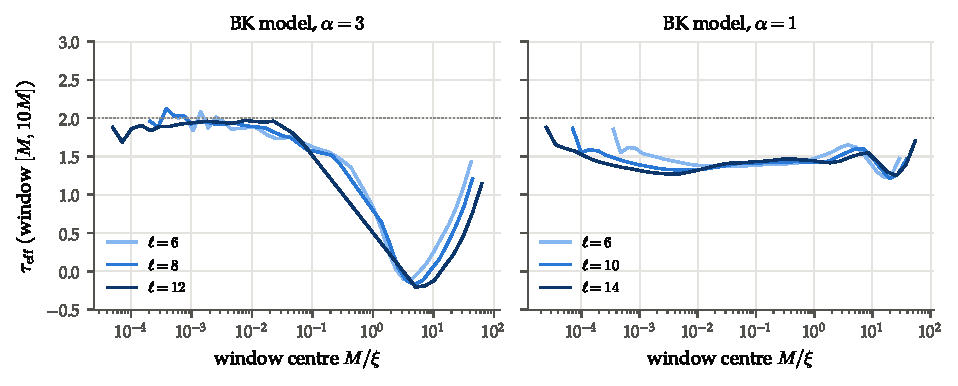
\includegraphics[width=\linewidth]{mapping/bk_effective.pdf}
  \caption{Effective exponent of the moment density of the BK model, from maximum-likelihood fits in windows $[M,10M]$. The dotted line marks
  $\tau=2$, i.e.\ $b=1$.}
  \label{fig:bk-effective}
\end{figure}

\subsection{The sandpile limit is periodic}

The sandpile models behave in a completely different way. Their dynamics, after a transient, is \emph{exactly periodic}: the same sequence of
avalanches repeats again and again. For $N=4096$ and $\ell=6$, the fixed-drop rule has a period of $\mapperFixed$ avalanches, during which the plate
advances by exactly $\mapperPlateFixed$, which is the drop $\Delta f = \mapdropAthreeLsix$, and every site topples on average $\mapperTopplingsFixed$ times.
The reason is simple. Every toppling changes the forces by a fixed amount, $-\Delta f$ at the toppling site and $+\ell^2\Delta f/\omega_j^2$ at its
neighbours, and the plate adds a uniform amount. Up to an overall shift, the forces therefore live on a discrete grid; since they are also bounded,
the deterministic dynamics can visit only a finite number of configurations and must eventually repeat itself. The number of topplings per period
follows from force balance: in one period each bulk site gains $\Delta f$ from the plate, so it must topple $n$ times with
$n\Delta f(1 - 2\ell^2/\omega^2) = \Delta f$, i.e.\ $n = 2\ell^2+1 = 73$ for $\ell = 6$.

The reset (OFC) rule is periodic as well (period $\mapperReset$ avalanches for the same parameters), but in a different way: it
\emph{synchronises}. Almost every avalanche topples nearly all sites of the chain once; the system fires as a whole, like the single block of
\cref{fig:single-block}. This synchronisation of OFC-type models under uniform deterministic driving is well known.

The BK model, by contrast, is chaotic. \Cref{fig:chaos} follows two copies of each model that start from configurations differing by $10^{-12}$ in the
position of a single block. In the BK model the difference stays at $10^{-12}$ until an event reaches the perturbed block, and then grows by ten orders
of magnitude within about one unit of plate displacement. In the sandpile the difference is simply carried along, without growing, for as long as we
follow it. This is the dynamical difference between the two models: the velocity-weakening instability of \cref{sec:bk-instability} continuously
generates new irregularities in the BK chain, while the inertia-free sandpile has no such source and settles on a periodic orbit.

\begin{figure}[t]
  \centering
  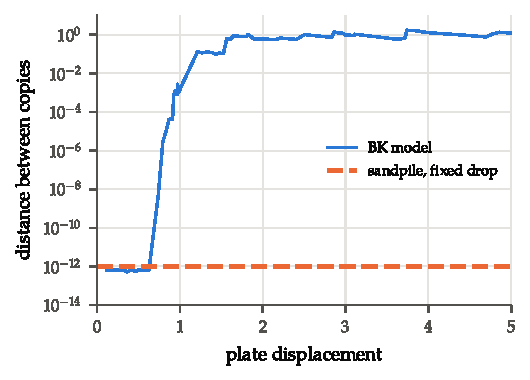
\includegraphics[width=0.55\linewidth]{mapping/chaos.pdf}
  \caption{Sensitivity to initial conditions. Distance between two copies of each model that initially differ by $10^{-12}$ in one block ($N=256$,
  $\ell=6$, $\alpha=3$, $\sigma=0.01$).}
  \label{fig:chaos}
\end{figure}

\subsection{Distributions}

\Cref{fig:compare} compares the distributions of the three models. The fixed-drop sandpile produces only small avalanches: their moments lie between that of a
one-block event and about $10^{-2}\xi$, and they involve at most a few tens of blocks (\cref{fig:blocks}), comparable to the stiffness length $\ell$. There is no
scaling region, no crossover and no delocalized events: the distribution is a single hump. The reset sandpile shows a few sharp spikes, the sizes that occur in its
synchronised cycle; the largest correspond to the whole chain slipping. Neither resembles the BK distribution, which extends continuously over more than seven
decades in moment.

\begin{figure}[t]
  \centering
  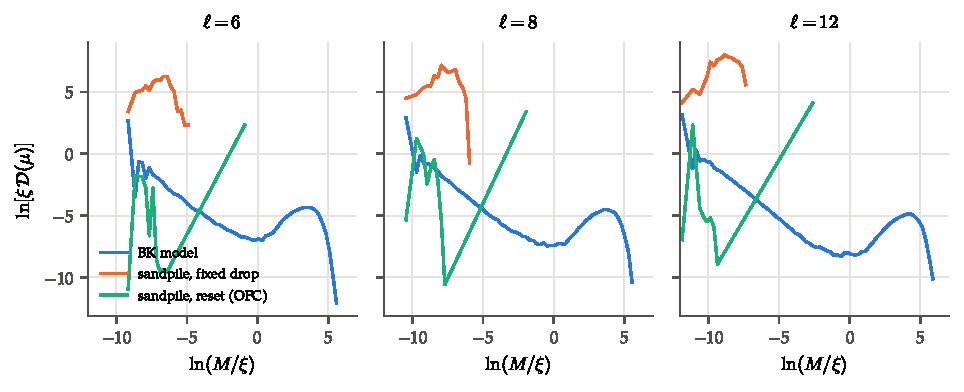
\includegraphics[width=\linewidth]{mapping/compare_alpha3.pdf}
  \caption{Frequency of events per unit magnitude, per unit length and per unit plate displacement, for the BK model and its two sandpile limits ($\alpha=3$,
  $\sigma=0.01$). The curves of the reset rule consist of a few spikes, the distinct sizes in its periodic, synchronised cycle.}
  \label{fig:compare}
\end{figure}

\begin{figure}[t]
  \centering
  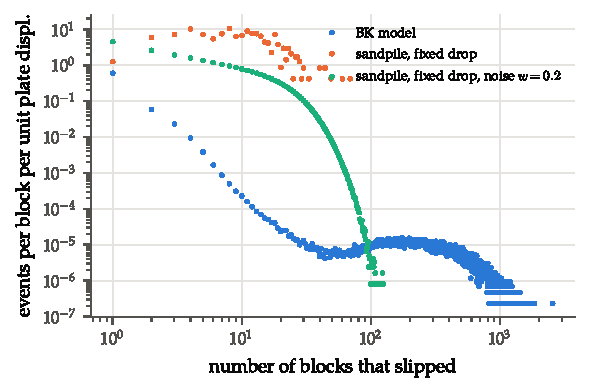
\includegraphics[width=0.62\linewidth]{mapping/blocks.pdf}
  \caption{Distribution of the number of blocks that slip in an event, for $\ell=6$, $\alpha=3$, $\sigma=0.01$.}
  \label{fig:blocks}
\end{figure}

\subsection{The test with \texorpdfstring{$\alpha$}{alpha}}

\Cref{sec:map-properties} predicted that in the sandpile limit the friction parameters only set the unit of slip. \Cref{fig:alpha-test} confirms this: for $\ell=6$, the
sandpile distributions for $\alpha=1$ and $\alpha=3$ nearly coincide once $\mu$ is measured relative to $\ln\Delta f$ (the remaining small differences come from the two
runs having settled on different periodic orbits). In the BK model the same change of $\alpha$ transforms the distribution: for $\alpha=3$ it has a steep scaling region and
a separate peak of large events, for $\alpha=1$ a single, much flatter power law. The dependence on $\alpha$, i.e.\ on how strongly a slipping block accelerates, is a
property of the inertial dynamics that the sandpile limit cannot represent.

\begin{figure}[t]
  \centering
  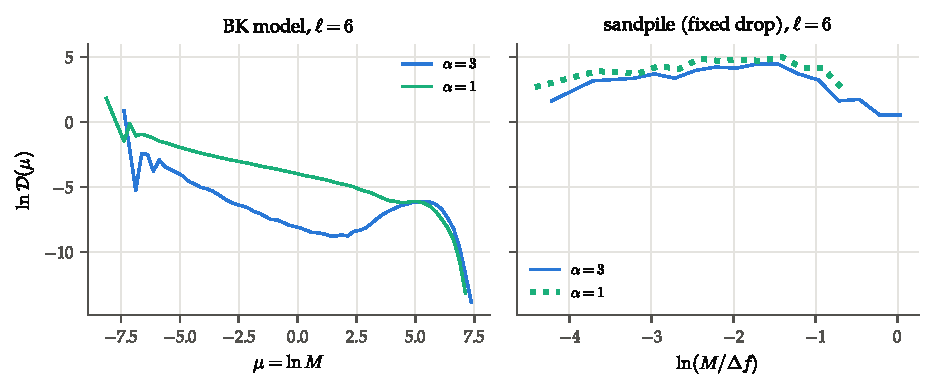
\includegraphics[width=\linewidth]{mapping/alpha_test.pdf}
  \caption{Changing the velocity weakening $\alpha$ at $\ell=6$, $\sigma=0.01$. Left: BK model. Right: fixed-drop sandpile, with moments measured in units of the drop
  $\Delta f$.}
  \label{fig:alpha-test}
\end{figure}

\subsection{Adding disorder}

The periodicity of the sandpile limit suggests a possible repair. In the BK model, irregularities are generated by the dynamics itself; in the sandpile
they could be supplied from outside. A common way to do this is to give the friction a random component: each block has its own static threshold
$\theta_j$, and after every slip it draws a new one, $\theta_j = 1+\eta$ with $\eta$ uniformly distributed in $[-w/2,w/2]$. This models a fault surface
whose strength varies from place to place and changes as the surface slides. We used $w = 0.01$, $0.05$ and $0.2$, i.e.\ from a quarter of the drop
$\Delta f$ to about five times it.

The noise destroys the periodicity of both rules, and for $w\ge0.05$ it also destroys the synchronisation of the reset rule. The distributions become smooth
(\cref{fig:noise}), but they remain bounded: even for the strongest noise the largest events involve $\mapnoiseMaxfixedsix$ blocks for $\ell=6$ and
$\mapnoiseMaxfixedtwelve$ for $\ell=12$ (fixed-drop rule), with moments below about $\mapnoiseMaxMfixedsix\,\xi$, and the mean number of blocks per event is
$\mapnoiseMeanfixedsix$ and $\mapnoiseMeanfixedtwelve$. The size of the largest events thus grows in proportion to the stiffness length, as expected from the bulk
dissipation $\epsilon = 1/(2\ell^2+1)$ discussed in \cref{sec:soc-implications}: a packet of force that loses a fraction $\epsilon$ at each toppling
travels a distance of order $\epsilon^{-1/2}\approx\sqrt2\,\ell$. None of the noisy sandpiles develops a scaling region, a crossover or delocalized events.

\begin{figure}[t]
  \centering
  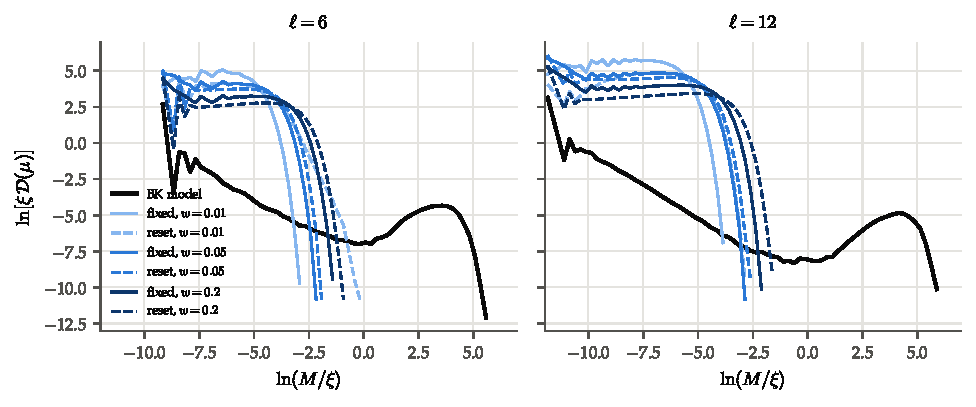
\includegraphics[width=\linewidth]{mapping/noise.pdf}
  \caption{The sandpile limit with random thresholds (noise width $w$), compared with the BK model ($\alpha=3$, $\sigma=0.01$). Solid: fixed-drop rule;
  dashed: reset rule.}
  \label{fig:noise}
\end{figure}

% ======================================================================
\section{What the mapping captures and what it misses}
\label{sec:map-discussion}

The comparison gives a clear answer to the question posed at the beginning of this chapter.

\paragraph{What survives.} The mapping is exact for the elementary process: an isolated toppling of the sandpile is, by construction, identical to a
one-block event of the BK model, including the velocity-weakening correction \cref{eq:map-drop}, and the smallest events of the two models agree to about 1\% (the remaining difference is the curvature of the friction law, which \cref{eq:map-drop} neglects). The
force bookkeeping \cref{eq:force-bookkeeping} and the sum rule are exact in both. The redistribution of the shed force, with the fraction
$\epsilon=1/(2\ell^2+1)$ lost into the pulling springs, is also the same.

\paragraph{What is lost.} Everything that depends on the \emph{motion} of the blocks is lost:
\begin{enumerate}
  \item \textbf{Amplification of slip.} In the BK model a slip that spreads gains energy, because velocity-weakening friction acts as a negative damping
    (\cref{sec:bk-pulses}). A group of blocks slips further than a single block, and a pulse that runs through a region near threshold grows exponentially.
    This is what produces the delocalized events and the localization length $\tilde\xi$. In the sandpile every toppling sheds the same small force,
    whatever its neighbours are doing, so avalanches cannot grow beyond the range set by the bulk dissipation, about $\ell$ blocks.
  \item \textbf{Self-generated disorder.} The same instability makes the BK model chaotic (\cref{fig:chaos}); the large events leave behind rough
    configurations whose smoothing produces the scaling region of localized events (\cref{sec:bk-events}). The inertia-free sandpile is not chaotic: it
    settles on a periodic orbit, and externally imposed disorder does not replace the missing amplification.
  \item \textbf{The dependence on $\alpha$.} Because the sandpile only knows the drop $\Delta f$, it cannot distinguish strong from weak velocity weakening,
    which in the BK model changes the exponent of the scaling region from $b\approx1$ to $b\approx0.4$.
\end{enumerate}

\paragraph{Conclusion.} The simple quasi-static mapping of the one-dimensional BK model onto a sandpile \emph{fails}: the sandpile limit is neither critical
nor chaotic, and it reproduces none of the features of the BK size distribution beyond the smallest events. The failure is not a matter of parameters or of
details of the toppling rule: both natural rules (fixed drop and OFC reset) fail, with and without noise. It is a consequence of removing inertia, which in
the BK model is the mechanism that makes events grow. A cellular-automaton description of the BK model would have to represent this amplification:
a slipping region gains momentum as it grows, and the blocks it reaches are pushed not only by the static forces of the springs but by moving
neighbours. Representing momentum requires carrying the velocities of the blocks from one step to the next, which brings back the full dynamics of
\cref{eq:bk}. In this sense the statistics of the BK model are intrinsically dynamical: they cannot be obtained from a sandpile built from static
force transfer alone.

\chapter{Numerical methods and validation}
\label{ch:numerics}

\newcommand{\valoneBlockA}{702.2}
\newcommand{\valoneBlockErrA}{2.5}
\newcommand{\valoneBlockMinA}{697}
\newcommand{\valoneBlockMaxA}{706}
\newcommand{\vallargeA}{6.20}
\newcommand{\vallargeErrA}{0.02}
\newcommand{\valoneBlockB}{700.8}
\newcommand{\valoneBlockErrB}{2.4}
\newcommand{\valoneBlockMinB}{697}
\newcommand{\valoneBlockMaxB}{705}
\newcommand{\vallargeB}{6.20}
\newcommand{\vallargeErrB}{0.03}
\newcommand{\valerrCascadeHA}{9.3e-08}
\newcommand{\valstatEventsA}{1{,}000{,}000}
\newcommand{\valstatEventsB}{1{,}000{,}000}


This chapter describes how the models of the previous chapters are simulated and how we know that the programs are
correct. The guiding principle is that no simulation result is used unless the program that produced it has first
reproduced known results: exact solutions, conservation laws, and an independent reference implementation. We describe
the software (\cref{sec:num-software}), the algorithms for the sandpile (\cref{sec:num-btw}), the BK model
(\cref{sec:num-bk}) and its sandpile limit (\cref{sec:num-mapped}), and the tests that each of them passes. The last
section (\cref{sec:num-legacy}) lists the errors found in the earlier version of this project, which motivated the complete
rewrite.

% ======================================================================
\section{Software}
\label{sec:num-software}

All programs are written in Python. The time-critical loops are compiled to machine code with Numba, which gives the speed of
C while keeping the code readable. The code is organised as a small package, \code{bksoc}, with one module per model:
\begin{center}
\begin{tabular}{@{}ll@{}}
\toprule
module & content \\
\midrule
\code{sandpile.py} & BTW sandpile on an arbitrary lattice (Chapter~\ref{ch:soc}) \\
\code{theory.py} & exact results for Abelian sandpiles, used as test references \\
\code{stats.py} & binning, maximum-likelihood fits, blocking, finite-size scaling (Chapter~\ref{ch:measuring}) \\
\code{bk.py} & Burridge--Knopoff chain (Chapter~\ref{ch:bk}) \\
\code{mapped.py} & sandpile limit of the BK chain (Chapter~\ref{ch:mapping}) \\
\bottomrule
\end{tabular}
\end{center}
Each figure of this thesis is produced by a script in \code{scripts/thesis/}, which runs the simulations, stores the raw results
together with a file of parameters and random seeds, and draws the figure; the numbers quoted in the text are written by the same
scripts. The test suite, \code{tests/}, contains 81 tests and runs in about a minute and a half. A single simulation always runs on one
processor core; independent runs (different parameters or seeds) are distributed over the cores of the machine. This is far more
efficient than parallelising one run, because the dynamics of an avalanche or an event is inherently sequential.

% ======================================================================
\section{The sandpile}
\label{sec:num-btw}

\paragraph{Algorithm.} The lattice is stored as a table of neighbours: row $i$ lists the $k$ neighbour slots of site $i$, and a slot
pointing outside the lattice is marked with $-1$. This one representation covers chains, square lattices and any other graph. An
avalanche is relaxed with the parallel update of \cref{sec:btw-def}: a list holds the sites that are unstable at the start of a time
step, all of them topple, and the sites made unstable by this are collected into the list for the next step. Each toppling costs a fixed
number of operations, so the cost of an avalanche is proportional to its size; on one core the program performs about $4\times10^7$
topplings per second.

\paragraph{Validation.} The tests check, in order of increasing strength:
\begin{itemize}[nosep]
  \item conservation of grains (grains added $=$ grains in the system $+$ grains lost);
  \item the Abelian property, by comparing every avalanche with an independent, slow implementation that topples unstable sites one at a
    time in \emph{random} order (same final configuration, size and area);
  \item the exact one-dimensional solution of \cref{sec:btw1d}, for every recurrent configuration and every seed, including the full
    toppling profile \cref{eq:n1d};
  \item the stationary size distribution of the chain, against the exact enumeration, with a $\chi^2$ test;
  \item the number of recurrent configurations, $\det\Delta$, by counting the states visited in a long run;
  \item the exact mean avalanche size \cref{eq:mean-s} and the height probabilities of the two-dimensional model (\cref{sec:btw2d}).
\end{itemize}

% ======================================================================
\section{The Burridge--Knopoff chain}
\label{sec:num-bk}

\subsection{The difficulty}

\Cref{eq:bk} is an ordinary differential equation, but not a smooth one: the friction force jumps when a block starts or stops slipping,
and a stuck block is not described by an equation of motion at all but by a constraint. Standard integrators with a fixed time step handle
such switches poorly. If a stop or a start is noticed only at the end of a time step, the error made in that step is proportional to the
step size $h$, whatever the order of the integrator. Since a large event contains thousands of such switches, they dominate the error.

\subsection{Algorithm}

The program treats stuck and slipping blocks separately.
\begin{enumerate}
  \item \textbf{Loading.} Between events all blocks are stuck. The program finds the block with the largest force $f_j$ and moves the plate
    exactly far enough that this force reaches 1 (for $\nu=0$; for $\nu>0$ the time advances by the corresponding amount). The block becomes
    \emph{active}.
  \item \textbf{Integration.} Only active (slipping) blocks are integrated, with the classical fourth-order Runge--Kutta method; stuck blocks
    stay exactly at rest. The cost of a time step is therefore proportional to the number of slipping blocks, not to $N$.
  \item \textbf{Stopping.} When the velocity of a slipping block changes sign during a step, the block sticks. Its position is corrected to the
    moment of the zero crossing, assuming constant acceleration within the step: if the velocity went from $V_0>0$ to $V_1\le0$, the crossing
    happened after a fraction $\theta = V_0/(V_0-V_1)$ of the step, and the block is placed at $U_0 + \tfrac12V_0\theta h$.
  \item \textbf{Starting.} After each step the program checks whether a stuck block has reached the threshold. If so, the moment of crossing is
    found by linear interpolation of its force between the beginning and the end of the step, and the block starts with the velocity and
    displacement it would have gained since that moment. This correction is what makes the method second-order accurate (see below).
  \item \textbf{Events.} An event is a cluster of slip that is connected in space and time. A block that starts to slip while one of its neighbours is
    slipping (or stopped in the same time step) joins that neighbour's event; otherwise it starts a new event, and two events that come into contact
    are merged. An event is over when its last block sticks. The program then records its moment, the number of distinct blocks that slipped, its
    duration, its epicentre, the plate position, and the energy dissipated by friction. For $\nu = 0$ the plate is frozen while blocks slip, so only
    one event can exist at a time and this definition reduces to ``everything between two loadings of the plate''. For $\nu>0$ several events can
    coexist in different parts of the chain, as in the simulations of Carlson and Langer (1989).
\end{enumerate}
With the 1989 friction law, a block whose velocity returns to zero while its force is still outside the static range simply starts again; following
Carlson and Langer, each such return of the velocity to zero ends one slip episode, so that the periodic small slips of a slowly creeping block are
counted as separate one-block events.
To find the block closest to the threshold without scanning all $N$ blocks, the forces of the stuck blocks are kept in a \emph{segment tree}, a
binary tree in which every node stores the largest value below it. Updating one force and finding the largest one both take a time proportional to
$\log N$. With these choices a chain of 4096 blocks runs at about $4\times10^4$ events per second; one unit of plate displacement takes between
0.2 seconds ($\ell=6$, $\alpha=3$) and a few seconds ($\ell=14$, $\alpha=1$, $N=8192$), because events are larger and last longer for stiffer chains and
weaker velocity weakening.

\paragraph{Time step.} The fastest motion in the chain is its highest normal mode, with angular frequency $\omega_{\max} = \sqrt{4\ell^2+1}$ (neighbouring
blocks moving in opposite directions). We use $h = 0.1/\omega_{\max}$, i.e.\ about 60 steps per period of the fastest oscillation.

\subsection{Validation}

\paragraph{Exact one-block events.} An isolated block reaching the threshold in a stuck chain must slip by $2\sigma/(2\ell^2+1)$ when velocity weakening is
switched off (\cref{eq:dU1}). The program reproduces this to seven significant digits, and the duration $\pi/\omega_1$ to the accuracy of the time step. With
velocity weakening it agrees with the solution of the single-block equation with the full nonlinear friction law to $10^{-4}$, and with the linearised
formula \cref{eq:dU1-alpha} to 2\%.

\paragraph{Comparison with a reference solver.} The most demanding test compares whole events with an independent implementation. The reference solver
integrates the equations of motion with an adaptive high-order method (Dormand--Prince of order 8, relative tolerance $10^{-11}$) and locates every stop and
every start exactly, by root finding on the velocity of each slipping block and on the force of each stuck block; between two such switches the set of slipping
blocks is fixed and the equations are smooth. The comparison uses chains of ten blocks prepared so close to threshold that the event cascades through all of
them. \Cref{fig:convergence} shows the largest difference in the final positions as a function of the time step: it decreases as $h^2$, and at $h=10^{-3}$ it is
$\valerrCascadeHA$, for slips of order one. During the development of the program, before the starting correction (item 4 above) was introduced, the same test
showed only first-order convergence, with errors about a thousand times larger.

\begin{figure}[t]
  \centering
  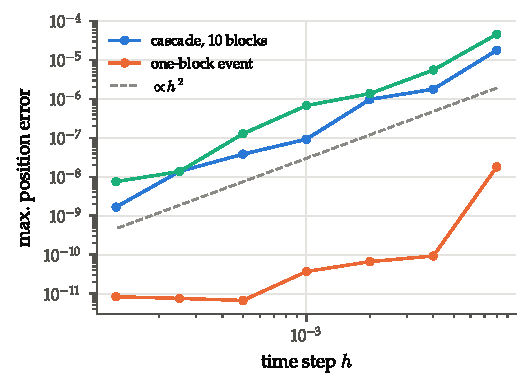
\includegraphics[width=0.58\linewidth]{validation/convergence.pdf}
  \caption{Error of the BK program against the reference solver, for single events in a chain of ten blocks. For one-block events the error reaches the tolerance of
  the reference solver.}
  \label{fig:convergence}
\end{figure}

\paragraph{Conservation laws.} With the plate at rest, the mechanical energy (kinetic energy plus the elastic energy of all springs) lost in an event must equal the
work done by friction, which the program accumulates with the same Runge--Kutta weights as the motion. Over thousands of events the two agree with a median relative
difference of $3\times10^{-7}$. The total moment of all events equals $N$ times the increase of the mean block position to machine precision, and the mean block
position stays within a bounded distance of the plate, as the sum rule requires.

\paragraph{Invariances.} No block ever moves backwards with the 1991 law, all forces are below the threshold after every event, the result is unchanged when the chain
is mirrored, and shifting all blocks and the plate by the same amount leaves the events unchanged. (In the last test only the first events are compared: the model is
chaotic, and differences of the order of the rounding error, $10^{-15}$, eventually grow to visible size.)

\paragraph{The 1989 friction law.} The reference solver was extended to the symmetric friction law, with backward slip and a moving plate. Whole cascades in
chains of eight blocks agree with it to $10^{-4}$ in the final positions. A block that reaches the threshold in a slowly loaded chain creeps with an
oscillating velocity; its first slip episode, of size about $2\pi\nu/\omega_1^3$, agrees with the exact single-block solution to $2\times10^{-3}$. This last
test exposed an error in an intermediate version of the program: within a Runge--Kutta step, a stage velocity slightly below zero made the symmetric friction
change sign and gave the block a spurious kick, so that creeping blocks ``bounced'' instead of stopping. Friction is now always evaluated against the current
direction of motion. Further tests check that every slip is assigned to an event (the moments of completed and unfinished events add up to the total slip
exactly), that no event is left unrecorded once all its blocks have stopped, that the number of blocks in an event never exceeds $N$, and that two blocks
reaching the threshold at the same time far apart produce two separate events. For a single block, the slip of each stick--slip cycle agrees with a direct
integration to $10^{-3}$.

\paragraph{Statistical convergence.} Because the dynamics is chaotic, individual trajectories computed with different time steps eventually diverge, and convergence must
be checked on the statistics. \Cref{fig:statistical} compares the distribution $\mathcal D(\mu)$ for $h = 0.1/\omega_{\max}$ and $h=0.05/\omega_{\max}$ ($N=1024$, $\ell=6$,
$\alpha=3$, $\sigma=0.01$, $10^6$ events each). The two curves are indistinguishable by eye, but a quantitative comparison taught us something about the errors. For all
magnitudes except the smallest the two runs agree within their statistical errors; the rate of one-block events, which make up 85\% of all events, differed by 2\%, many
times its error estimated by blocking the time series into 50 pieces. To decide whether this was an effect of the time step, we repeated the runs with three independent
initial conditions for each time step (600 units of plate displacement each). The rate of one-block events per unit plate displacement varies between runs from
$\valoneBlockMinA$ to $\valoneBlockMaxA$ for the larger step and from $\valoneBlockMinB$ to $\valoneBlockMaxB$ for the smaller one; the averages, $\valoneBlockA\pm\valoneBlockErrA$
and $\valoneBlockB\pm\valoneBlockErrB$, agree, as do the rates of large events ($M>6$), $\vallargeA\pm\vallargeErrA$ and $\vallargeB\pm\vallargeErrB$. The time step
therefore has no detectable effect on the statistics. The difference seen in the first comparison is a run-to-run fluctuation: the rate of small events depends on the
slowly evolving roughness of the chain, whose memory is longer than the blocks used in the first error estimate. For quantities of this kind we estimate errors from
independent runs.

\begin{figure}[t]
  \centering
  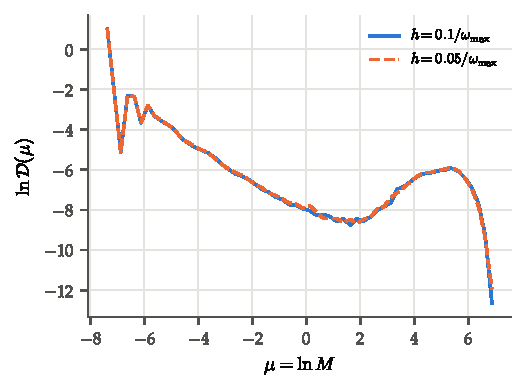
\includegraphics[width=0.58\linewidth]{validation/statistical.pdf}
  \caption{Distribution of event magnitudes of the BK model computed with two time steps.}
  \label{fig:statistical}
\end{figure}

% ======================================================================
\section{The sandpile limit}
\label{sec:num-mapped}

The program for the sandpile limit of Chapter~\ref{ch:mapping} combines the two previous ones: the forces $f_j$ are relaxed with the parallel update of the sandpile,
and the plate is moved as in the BK program, with a segment tree to find the next block to reach the threshold. It performs between $5\times10^5$ and $10^6$ avalanches per
second for the chains used here. The tests check that the fixed-drop rule is Abelian (against a random-order reference implementation), that the force bookkeeping
\cref{eq:force-bookkeeping} holds to rounding precision, that all forces are below the threshold after every avalanche, that an isolated toppling with the drop
\cref{eq:map-drop} reproduces the one-block event of the BK program, that changing the drop only changes the unit of slip, and that threshold noise breaks the
periodicity without violating the force bookkeeping.

% ======================================================================
\section{Statistical tools}
\label{sec:num-stats}

The methods of Chapter~\ref{ch:measuring} are tested on synthetic data with known answers: the maximum-likelihood estimates (continuous, discrete and truncated) recover
the exponents used to generate the data within their error bars, and the error bars themselves are correct (68\% coverage); the discrete sampler reproduces the exact
probabilities; the choice of $x_{\min}$ finds the onset of a power-law tail; the goodness-of-fit test accepts a power law and rejects an exponential; the blocking
method reproduces the exact error of the mean of a correlated (autoregressive) process; and the moment analysis and data collapse recover the exponents of synthetic
finite-size-scaling data, including the exact corrections to scaling.

% ======================================================================
\section{The earlier implementation}
\label{sec:num-legacy}

The earlier version of this project did not reproduce the results of Carlson and Langer. A review of its code, carried out before the rewrite, found the following
problems. They are listed because each of them is a mistake that is easy to make and hard to notice without tests of the kind described above.
\begin{enumerate}
  \item \textbf{An error in the Runge--Kutta step.} The fourth stage used $v + \tfrac12k_3$ instead of $v + h\,k_3$ for the velocity, so the integration was not of
    fourth order; in fact it was not consistent at all for the positions.
  \item \textbf{Stiffness tied to the system size.} The pulling-spring constant was set to $k_p = 1/(L-1)$, with $L$ the number of blocks, so that changing the length of
    the chain also changed the stiffness ratio $\ell^2$.
  \item \textbf{Units.} The program used units in which $k_c = m = F_0 = 1$, while the friction parameter was compared directly with the $\alpha$ of the papers. As shown in
    \cref{sec:bk-units}, a friction coefficient $c$ in such units corresponds to $\alpha = c/(2\sqrt{k_p})$, e.g.\ $\alpha=2.5\,c$ for $k_p = 0.04$.
  \item \textbf{Boundary conditions.} The missing neighbours of the end blocks were set to zero displacement, which attaches the chain to fixed walls, instead of the free ends
    of the papers.
  \item \textbf{Stick--slip handling.} The friction law was evaluated inside the Runge--Kutta stages with the static or kinetic branch chosen from intermediate velocities,
    and negative velocities were simply set to zero at the end of each step, without locating the stopping time. Starts of slip were detected only at the end of a step.
  \item \textbf{Event durations.} In the GPU version the array of times was never filled, so all event durations were recorded as zero.
\end{enumerate}
Each of these would be caught immediately by one of the tests of \cref{sec:num-bk}: the one-block event, the comparison with the reference solver, or the energy balance.

\chapter{Results: reproduction and the question of criticality}
\label{ch:results}

\newcommand{\resoffMeanG}{1.6}
\newcommand{\ressumOursG}{1.01}
\newcommand{\ressumTheirsG}{0.21}
\newcommand{\resoffMeanBC}{1.6}
\newcommand{\ressumOursBC}{1.00}
\newcommand{\ressumTheirsBC}{0.20}
\newcommand{\resMstarExp}{0.95}
\newcommand{\restauEllG}{1.96}
\newcommand{\reserrEllG}{0.01}
\newcommand{\restauEllI}{1.92}
\newcommand{\reserrEllI}{0.00}
\newcommand{\restauEllBC}{1.91}
\newcommand{\reserrEllBC}{0.00}
\newcommand{\restauEllBG}{1.88}
\newcommand{\reserrEllBG}{0.00}
\newcommand{\restauEllCE}{1.87}
\newcommand{\reserrEllCE}{0.01}
\newcommand{\reslenLongA}{4008}
\newcommand{\reslenLongB}{2000}
\newcommand{\reslenLongC}{2000}
\newcommand{\reslenLongD}{2001}
\newcommand{\reslenLongE}{2010}


This chapter collects the results on the Burridge--Knopoff model itself. \Cref{sec:res-1991} completes the comparison with Carlson,
Langer, Shaw and Tang (1991) begun in Chapter~\ref{ch:mapping}, including a discrepancy in the normalisation of their figures.
\Cref{sec:res-sigma,sec:res-ell} address the question of whether the model is critical, by varying the friction drop $\sigma$ (which
Carlson \emph{et al.} identify as the critical parameter) and the stiffness $\ell$ (which controls the approach to the continuum limit).
\Cref{sec:res-1989} reproduces the 1989 study of Carlson and Langer, and \cref{sec:res-summary} summarises what has been learned. All
simulations use the programs of Chapter~\ref{ch:numerics}, and all distributions are normalised per unit length and per unit plate
displacement (\cref{sec:bk-stats}).

% ======================================================================
\section{The 1991 model}
\label{sec:res-1991}

\subsection{Shape and exponents}

Chapter~\ref{ch:mapping} showed that our simulations reproduce the features of the size distributions of Carlson \emph{et al.}: peaks of
one- and few-block events, a scaling region of localized events, a minimum near $M=\xi$, a rising branch of delocalized events and a sharp
upper cutoff (\cref{fig:compare,fig:bk-effective}). The exponents of the scaling region agree with theirs: $b = 0.96$, $0.92$ and $0.91$ for
$\ell = 6$, 8 and 12 at $\alpha = 3$ (theirs: $0.92$), and $b\approx0.36$--$0.40$ for $\alpha = 1$ (theirs: $0.35$). The positions of the
minimum and of the peak of delocalized events agree with their Fig.~3 to within a few tenths in $\ln(M/\xi)$.

\subsection{Normalisation}

There is, however, a difference in the \emph{height} of the distributions. \Cref{fig:normalisation} compares our results with values read off
Fig.~3 of Carlson \emph{et al.} at three landmarks: a point in the scaling region, the minimum, and the peak of delocalized events. For both
$\ell = 6$ and $\ell = 12$ their curves lie below ours by an almost constant amount, $\Delta\ln(\xi\mathcal D)\approx\resoffMeanG$, i.e.\ a factor
of about $e^{1.6}\approx5$. A constant vertical offset on a logarithmic plot means the same distribution with a different normalisation.

The sum rule decides which normalisation is the one defined in their paper. In the coordinates of the figure, $x=\ln(M/\xi)$ and
$y=\ln(\xi\mathcal D)$, we have $M = \xi e^x$, $\mathcal D = e^y/\xi$ and $\dd\mu = \dd x$, so the sum rule \cref{eq:sumrule} reads
\begin{equation}
  \int M\,\mathcal D(\mu)\,\dd\mu = \int e^{x+y}\,\dd x = 1 .
\end{equation}
This integral can be evaluated directly from a plotted curve. For our distributions it gives $\ressumOursG$ ($\ell = 6$) and $\ressumOursBC$
($\ell=12$), as it must. For curves lying $\resoffMeanG$ lower, as in their figure, it gives about $\ressumTheirsG$. The distributions plotted by
Carlson \emph{et al.} therefore do not satisfy their own sum rule (their Eq.~4.1); they appear to be normalised differently from their stated
definition by a factor of about five. We cannot identify the origin with certainty from the paper. A combination of two common conventions would
produce a factor of this size: measuring plate displacement in loading periods $2/\nu$ (a factor 2) and binning in $\log_{10}M$ while plotting
against $\ln M$ (a factor $\ln10\approx2.3$) together give $2\ln10\approx4.6$, i.e.\ $\Delta\ln\approx1.5$. Whatever its origin, the offset is
the same for all values of $\ell$ and does not affect any of the exponents or positions, which are the physically meaningful content of the comparison.

\begin{figure}[t]
  \centering
  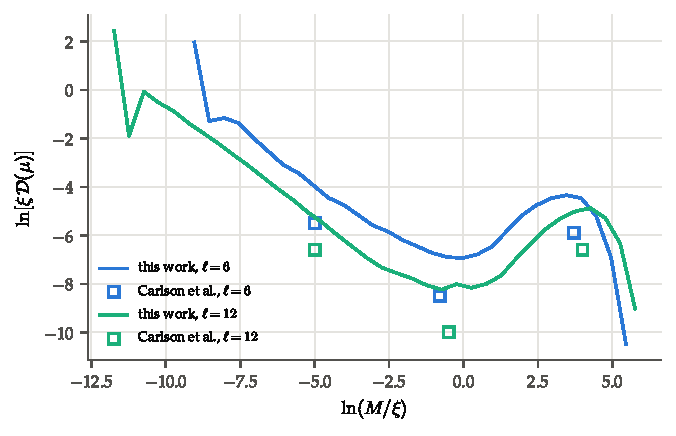
\includegraphics[width=0.62\linewidth]{results/normalisation.pdf}
  \caption{Our distributions for $\alpha=3$, $\sigma=0.01$ (lines) and three landmark values read from Fig.~3 of Carlson \emph{et al.} (1991)
  (squares).}
  \label{fig:normalisation}
\end{figure}

% ======================================================================
\section{Is the model critical? The role of \texorpdfstring{$\sigma$}{sigma}}
\label{sec:res-sigma}

\subsection{The hypothesis}

Carlson \emph{et al.} identify the friction drop $\sigma$ as the critical parameter of the 1991 model: the localization length
$\tilde\xi = (2\xi/\alpha)\ln(4\ell^2/\sigma)$ (\cref{eq:xi-tilde}) diverges as $\sigma\to0$, so that in this limit the range of localized events would
become infinite, as at a critical point. At the same time, their estimate of the crossover moment, $\tilde M = 2\xi/\alpha$, does not depend on $\sigma$.
To test this picture we simulated the model with $\alpha=3$, $\ell=6$, $N=4096$ and $\sigma$ from 0.1 down to 0.0003, each over 1000 units of plate
displacement.

\subsection{Results}

\Cref{fig:sigma} and \cref{tab:sigma} show the results. Two things are clear.

\emph{The small events depend on $\sigma$.} The one-block moment $M_1$ is proportional to $\sigma$, and as $\sigma$ decreases the distribution extends to ever
smaller moments, with the peaks of one- and few-block events moving with it (left panel). These microscopic events make the effective exponent oscillate
in the lower part of the range (middle panel).

\emph{Everything else does not.} For $\sigma\le0.03$ the distributions of moments coincide for $M\gtrsim0.03\,\xi$, and the distributions of the number of
blocks per event coincide for events of more than about ten blocks (right panel). The rate of events with ten or more blocks, the position of the minimum
of $\mathcal D(\mu)$ ($M\approx0.85\,\xi$), the position $\Delta_{\min}$ of the minimum of the block-number distribution, and the upper cutoff of the delocalized
events are all independent of $\sigma$ within the accuracy of the data. In particular, $\Delta_{\min}$ stays between 45 and 57 blocks without any trend, while the prediction for
$\tilde\xi$ grows from 34 to 52.

\begin{figure}[t]
  \centering
  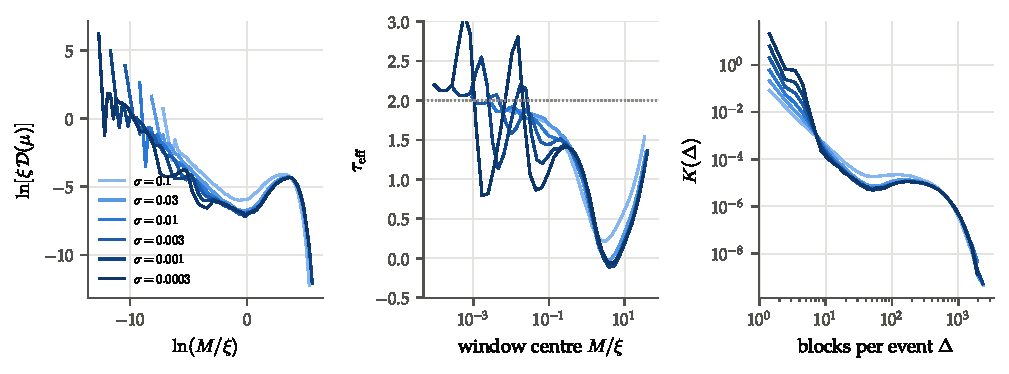
\includegraphics[width=\linewidth]{results/sigma_scan.pdf}
  \caption{The role of the friction drop $\sigma$ ($\alpha=3$, $\ell=6$, $N=4096$). Left: size distributions. Middle: effective exponent of the moment
  density in windows $[M,10M]$. Right: distribution of the number of blocks per event, per unit plate displacement and unit length.}
  \label{fig:sigma}
\end{figure}

\begin{table}[t]
\centering
\caption{Dependence on $\sigma$ ($\alpha=3$, $\ell=6$). $M_1$: one-block moment; $r_{10}$: events with at least ten blocks per block and per unit plate
displacement; $M_{\min}$: minimum of $\mathcal D(\mu)$; $\Delta_{\min}$: minimum of the block-number distribution; $\tilde\xi$: prediction
\cref{eq:xi-tilde}; $M^*$: 99th percentile of the delocalized events.}
\label{tab:sigma}
\begin{tabular}{ccccccc}
\toprule
$\sigma$ & $M_1$ & $r_{10}$ & $M_{\min}/\xi$ & $\Delta_{\min}$ & $\tilde\xi/a$ & $M^*/\tilde M$ \\
\midrule
\tabinput{figures/results/sigma_table.tex}
\bottomrule
\end{tabular}
\end{table}

\subsection{Interpretation}

The friction drop $\sigma$ controls only how small events can be; it does not control a length that grows as $\sigma\to0$. The statistics of all events of
more than a few blocks, localized and delocalized, are independent of $\sigma$ over the range studied, and no growing localization length is visible. In the
sense of \cref{sec:critical}, $\sigma$ is therefore not a critical parameter of the large-event statistics: making it smaller does not bring the model closer to
a scale-free state; it only adds microscopic events at the bottom of the distribution.

This also qualifies the ``Gutenberg--Richter'' scaling region of Carlson \emph{et al.} At $\sigma = 0.01$ the region with $b\approx1$ lies where the
$\sigma$-dependent few-block events overlap with the $\sigma$-independent localized events. Its effective exponent is not a property of the localized events
alone, and it shifts when $\sigma$ changes.

% ======================================================================
\section{Towards the continuum limit: the role of \texorpdfstring{$\ell$}{l}}
\label{sec:res-ell}

The other natural limit is $\ell\to\infty$ at fixed $\sigma$: the stiffness length $\xi=\ell a$ becomes large compared with the block spacing, and the chain
approaches the continuum equation \cref{eq:bk-cont}. Carlson \emph{et al.} argue that real faults have $\ell\sim100$. We extended their range $\ell = 6$--12 to
$\ell = 16$ and 24, with chains long enough that the largest events stay well below the system size (\cref{tab:ell}). Doubling the chain at $\ell=12$ (from 8192 to
16384 blocks) changes the upper cutoff by about 6\%, which shows that the runs at $\ell\le12$ are only marginally affected by the system size.

\begin{figure}[t]
  \centering
  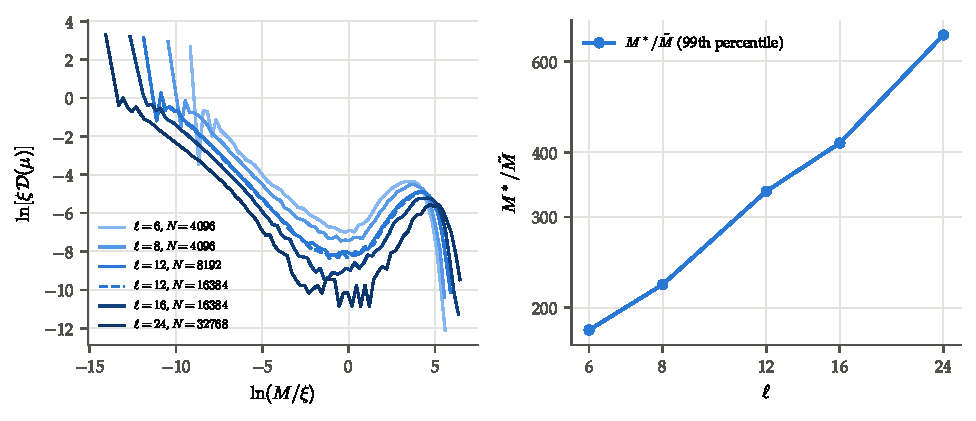
\includegraphics[width=\linewidth]{results/ell_scan.pdf}
  \caption{Approaching the continuum limit ($\alpha=3$, $\sigma=0.01$). Left: size distributions for $\ell$ from 6 to 24. Right: upper cutoff of the delocalized
  events, in units of $\tilde M = 2\xi/\alpha$.}
  \label{fig:ell}
\end{figure}

\begin{table}[t]
\centering
\caption{Dependence on $\ell$ ($\alpha=3$, $\sigma=0.01$): number of blocks, largest event (blocks), upper cutoff $M^*/\tilde M$, and the exponent of the localized
region from a maximum-likelihood fit between $\max(10M_1,10^{-4}\xi)$ and $10^{-2}\xi$.}
\label{tab:ell}
\begin{tabular}{ccccc}
\toprule
$\ell$ & $N$ & largest event & $M^*/\tilde M$ & $\tau$ \\
\midrule
\tabinput{figures/results/ell_table.tex}
\bottomrule
\end{tabular}
\end{table}

Two trends are visible (\cref{fig:ell}). First, the ratio of the upper cutoff of the delocalized events to the crossover moment grows with $\ell$, as
$M^*/\tilde M\propto\ell^{\resMstarExp}$, consistent with the rough proportionality to $\ell$ reported by Carlson \emph{et al.} The range of great events,
measured in units of the crossover, therefore grows without bound in the continuum limit. Because this ratio depends on $\ell = \xi/a$ and not on $\xi$ alone,
the block spacing remains relevant: as Carlson \emph{et al.} noted, the model has no simple continuum limit. Second, the window of the localized power law widens
(its lower end, $M_1/\xi\propto\sigma/\ell^3$, moves down), while its exponent decreases slowly, from $\tau = \restauEllG$ at $\ell=6$ to $\restauEllCE$ at $\ell=24$
($b$ from 0.96 to 0.87). Whether the exponent converges to a limiting value as $\ell\to\infty$ cannot be decided from this range.

% ======================================================================
\section{The 1989 model}
\label{sec:res-1989}

\subsection{Set-up}

The first study of Carlson and Langer~\cite{CarlsonLanger1989} used the symmetric friction law \cref{eq:phi89}, a finite loading speed $\nu$,
$\ell = 10$, and chains of 100 or 400 blocks. Their Fig.~6 shows distributions for five parameter sets, each obtained from one run of a given
length $T$ in loading periods $2/\nu$. We simulated each parameter set in two ways: as one long run, 4 to 44 times longer than theirs, and as five
independent runs of exactly their length. Events are space--time connected clusters of slip (\cref{sec:num-bk}); as in their analysis, each return
of a block's velocity to zero ends its slip episode, so that the small oscillating slips of a slowly creeping block count as separate one-block events.
With a finite loading speed the natural frequency of events is $\mathcal R(\mu)$, the number per unit time and unit length.

\subsection{Results}

\Cref{fig:cl1989} shows the distributions. All the features of their Fig.~6 are present. The tallest peak is that of one-block events, at the
magnitude $\mu_1 = \ln[2\pi\nu(2\ell^2)^{-3/2}]$ predicted by their small-event analysis ($-10.7$ for $\nu=0.01$ and $-13.0$ for $\nu=0.001$), followed by
peaks of few-block events. Then comes a straight scaling region, a minimum near $\mu\approx0$--1, and a peak of great events just below the largest
possible magnitude $\mu_L = \ln(2N)$ (dotted lines). For $\alpha=1$ (panel d) the scaling region is much flatter and the great events are weak, and for
$N=400$ (panel c) the peak of great events is lower and broader than for $N = 100$, both as in their figure.

\begin{figure}[t]
  \centering
  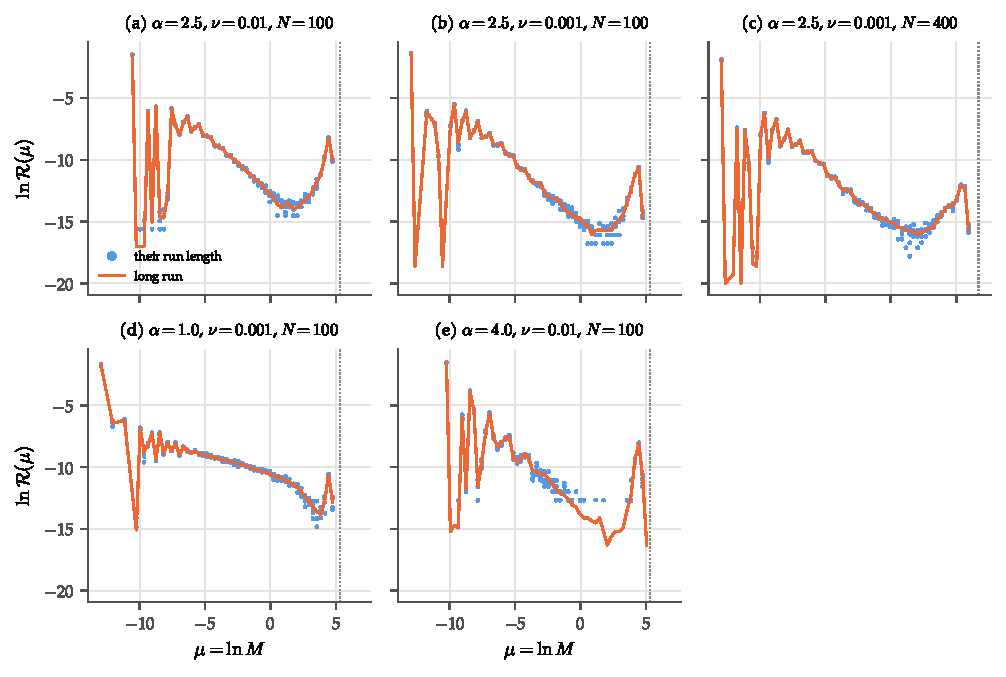
\includegraphics[width=\linewidth]{results/cl1989.pdf}
  \caption{The 1989 model with the parameters of Fig.~6 of Carlson and Langer ($\ell = 10$). Points: five independent runs of their length; line: one long
  run. Dotted line: $\mu_L=\ln(2N)$.}
  \label{fig:cl1989}
\end{figure}

\Cref{tab:cl1989} gives the exponent $b$ of the scaling region, from maximum-likelihood fits in $e^{-5}<M<e^{-1}$ ($e^{-7}<M<e^{2}$ for $\alpha=1$).
For $\alpha = 2.5$ we find $b = 0.89$--$0.94$, and for $\alpha = 1$, $b=0.29$, in reasonable agreement with their values $b\approx1$ and $b\approx0.35$
(their Fig.~7). For $\alpha=4$ we find $b = 0.80$, whereas their Fig.~7 gives $b\approx1$ for all $\alpha\ge2.5$.

\begin{table}[t]
\centering
\caption{The 1989 model: exponent $b$ of the scaling region from one long run, and its range over five independent runs of the original length $T$
(in loading periods).}
\label{tab:cl1989}
\begin{tabular}{cccccc c}
\toprule
 & $\alpha$ & $\nu$ & $N$ & $T$ & $b$ (long run) & $b$ (runs of length $T$) \\
\midrule
\tabinput{figures/results/cl1989_table.tex}
\bottomrule
\end{tabular}
\end{table}

\subsection{How much data did the 1989 study need?}

The five independent runs of the original length show how precisely the published distributions could be determined. For panels (a)--(d) the
small and intermediate events are well determined at the original length, and the spread of $b$ between runs is a few hundredths. The great events
are a different matter: they occur roughly once per loading period, so a run of 45 or 50 loading periods (panels d and e) contains only a few dozen of
them, and their part of the distribution differs visibly from run to run. For $\alpha = 4$ (panel e) even the exponent of the scaling region varies between
0.71 and 0.90 among runs of the original length, so their value $b\approx1$ at large $\alpha$ is within the statistical uncertainty of a single short run but
is not confirmed by our long run. This supports the suspicion, raised at the beginning of this project, that some of the published distributions were based
on too little data.

The main obstacle to reproducing the 1989 paper in the earlier version of this project was, however, not the length of the runs but the implementation
(\cref{sec:num-legacy}) and the definition of events. With a finite loading speed, slip somewhere in the chain is almost never absent, and defining an event as
``everything between two quiet periods'' merges unrelated slips into a few huge events; the space--time cluster definition, with each zero of a block's
velocity ending its episode, is needed to recover the distributions of Carlson and Langer.

% ======================================================================
\section{Summary: is the Burridge--Knopoff model critical?}
\label{sec:res-summary}

The results of this chapter and of Chapter~\ref{ch:mapping} answer the question in several parts.
\begin{enumerate}
  \item \textbf{There are power laws.} Localized events follow a power law with $b\approx0.9$ ($\tau\approx1.9$) for strong velocity weakening and
    $b\approx0.3$--$0.4$ for $\alpha=1$, over one to several decades in moment, in both the 1989 and the 1991 versions of the model.
  \item \textbf{Their range is set by the model, not by the system size.} The localized power law ends at a crossover moment $\tilde M\approx\xi$, and the
    great events have a cutoff $M^*\propto\ell^{\resMstarExp}\tilde M$; once the chain is several times longer than the largest event, the distributions no longer
    depend on its length. In SOC proper, by contrast, the only cutoff is the system size.
  \item \textbf{The friction drop $\sigma$ is not a critical parameter.} Reducing $\sigma$ by a factor of 100 (from 0.03 to 0.0003) changes only the smallest events; the statistics of all events
    of more than a few blocks, and the crossover length, stay the same.
  \item \textbf{The continuum limit $\ell\to\infty$ widens the windows.} Both the localized power law and the range of great events grow with $\ell$, while the exponent
    of the localized region drifts slowly ($\tau$ from 1.96 to 1.87 between $\ell = 6$ and 24). The block spacing remains relevant, so the model has no simple continuum
    limit.
  \item \textbf{The great events are characteristic, not critical.} They form a separate population with a peak and a sharp cutoff, which is the opposite of scale
    invariance, and they are produced by the inertial amplification of slip that the sandpile limit lacks (Chapter~\ref{ch:mapping}).
\end{enumerate}
The one-dimensional Burridge--Knopoff model is therefore not self-organized critical in the strict sense. It produces Gutenberg--Richter-like statistics over a window
bounded below by the microscopic events and above by a crossover set by the stiffness length, together with an excess of characteristic great events. The parameter that
controls how wide this window is, is the stiffness ratio $\ell$, i.e.\ the separation between the block spacing and the stiffness length, and not the friction drop or the
loading speed.

\chapter{Approximate theory}
\label{ch:theory}

\newcommand{\thampBK}{23}
\newcommand{\thampRigid}{81}
\newcommand{\thampSand}{4.5}
\newcommand{\thsandAsix}{1.45}
\newcommand{\thsandSsix}{1.96}
\newcommand{\thsandDecaysix}{1.21}
\newcommand{\thsandTausix}{0.92}
\newcommand{\thsandAtwelve}{1.25}
\newcommand{\thsandStwelve}{2.23}
\newcommand{\thsandDecaytwelve}{1.21}
\newcommand{\thsandTautwelve}{0.93}
\newcommand{\thonsetsix}{1.36}
\newcommand{\thonsettwelve}{1.69}
\newcommand{\thMcMin}{0.62}
\newcommand{\thMcMax}{0.85}
\newcommand{\thMcLmin}{3.8}
\newcommand{\thMcLmax}{6.6}
\newcommand{\thMcXiLsix}{0.78}
\newcommand{\thMcXiLtwentyfour}{0.16}


The previous chapters established, by simulation, what the Burridge--Knopoff (BK) model and its sandpile limit do. This chapter asks how much of
it can be understood with simple approximate calculations. We develop three approximations, each aimed at one question, and test each against
the simulations:
\begin{enumerate}
  \item \emph{What is the statistics of the sandpile limit?} The natural first approximation for any avalanche model is a branching process, the
    mean-field theory of avalanches (\cref{sec:th-branching}). We derive its size distribution exactly, apply it to the mapped sandpile of
    Chapter~\ref{ch:mapping}, and compare it with a second, one-dimensional approximation, a random walk with losses (\cref{sec:th-randomwalk}).
  \item \emph{Why do events in the BK model grow?} We extend the rigid-group calculation of \cref{sec:one-block-event} to include velocity
    weakening, which shows that the slip per block grows rapidly with the size of the slipping group and runs away above a size $n^*$
    (\cref{sec:th-amplification}).
  \item \emph{When are there great events, and where does the crossover lie?} Combining $n^*$ with the localization length $\tilde\xi$ of Carlson
    \emph{et al.} gives a criterion for the existence of a separate population of great events, which we test with new runs in which $\alpha$ and $\ell$
    are varied (\cref{sec:th-bimodal}). We also test the predicted crossover moment $\tilde M = 2\xi/\alpha$ (\cref{sec:th-crossover}).
\end{enumerate}
\Cref{sec:th-exponent} discusses what none of these approximations explains, the exponent of the localized events, and \cref{sec:th-summary}
summarises. All BK runs of this chapter use the 1991 friction law with $\sigma = 0.01$ and $\nu\to0$, the programs of Chapter~\ref{ch:numerics},
and the normalisation of \cref{sec:bk-stats}.

% ======================================================================
\section{Mean-field theory: the branching process}
\label{sec:th-branching}

\subsection{Definition}

Consider an avalanche as a family tree. The first toppling is the \emph{root}. Each toppling may cause further topplings, its
\emph{offspring}, by pushing neighbouring sites over the threshold; each of these may have offspring of its own, and so on. The avalanche ends
when a generation has no offspring. The \emph{size} $s$ of the avalanche is the total number of topplings, i.e.\ the number of members of the
tree.

The \emph{branching-process approximation} assumes that every toppling has offspring independently of all others, with the same probabilities
$p_k$ of having $k = 0,1,2,\dots$ offspring. This ignores the geometry of the lattice: in a real sandpile two topplings can push the same site,
and a site that has already toppled is less likely to topple again. The approximation becomes exact on a lattice of very high dimension, where
the chance of two branches meeting vanishes, and is therefore called the \emph{mean-field} theory of avalanches.

The most important parameter is the mean number of offspring, the \emph{branching ratio}
\begin{equation}
  m = \sum_k k\,p_k .
\end{equation}
The mean number of topplings in generation $g$ is $m^g$: the root is generation 0, it has on average $m$ offspring, each of which has on average
$m$ offspring, and so on. The mean size is therefore
\begin{equation}
  \avg{s} = \sum_{g=0}^\infty m^g = \frac{1}{1-m}\qquad(m<1),
  \label{eq:bp-mean}
\end{equation}
which diverges as $m\to1$. A process with $m<1$ is \emph{subcritical} (avalanches die out quickly), one with $m>1$ is \emph{supercritical}
(with a finite probability the avalanche never stops), and $m = 1$ is the \emph{critical} branching process. The branching ratio plays the
role of the control parameter of \cref{sec:critical}.

\subsection{The size distribution}

We now compute the full distribution $P(s)$ for the simplest case, \emph{binary branching}: each toppling has either no offspring (probability
$1-p$) or two (probability $p$). Then $m = 2p$, and the critical point is $p=1/2$. Every tree has an odd size, since each branching adds two members.

\paragraph{Small trees by hand.} An avalanche of size 1 is a root without offspring, with probability $1-p$. An avalanche of size 3 is a root
with two offspring, both of which have none: probability $p(1-p)^2$. For size 5 the root has two offspring, and exactly one of them has two
offspring, all others none; there are two such trees (the left or the right child branches), so $P(5) = 2p^2(1-p)^3$. In general, a tree of size
$s = 2k+1$ contains $k$ branching members and $k+1$ childless ones, so each such tree has probability $p^k(1-p)^{k+1}$, and
\begin{equation}
  P(2k+1) = C_k\,p^k(1-p)^{k+1},
\end{equation}
where $C_k$ is the number of different binary trees with $k$ branching members. The first values are $C_0 = C_1 = 1$, $C_2 = 2$.

\paragraph{The generating function.} To find $C_k$ in general we use the \emph{generating function} $Q(x) = \sum_s P(s)\,x^s$, a power series
whose coefficients are the probabilities. It satisfies a simple equation. A tree is either a single childless root, which contributes $(1-p)x$,
or a root with two offspring, each of which is the root of an independent tree of the same kind. Since the size of the whole tree is $1$ plus the
sizes of the two subtrees, and the generating function of a sum of independent sizes is the product of the generating functions, this second case
contributes $p\,x\,Q(x)^2$. Hence
\begin{equation}
  Q = (1-p)\,x + p\,x\,Q^2 .
\end{equation}
This is a quadratic equation for $Q$, with the solution
\begin{equation}
  Q(x) = \frac{1 - \sqrt{1-4p(1-p)\,x^2}}{2px}
\end{equation}
(the other root diverges as $x\to0$ and is excluded because $Q(0) = 0$). Expanding the square root in powers of $y = 4p(1-p)x^2$ with the binomial
series $\sqrt{1-y} = 1-\sum_{k\ge0}\frac{(2k)!}{(k!)^2(k+1)\,2^{2k+1}}\,y^{k+1}$ and collecting the coefficient of $x^{2k+1}$ gives
\begin{equation}
  C_k = \frac{(2k)!}{k!\,(k+1)!},
  \label{eq:catalan}
\end{equation}
the Catalan numbers $1,1,2,5,14,\dots$, in agreement with the trees counted by hand.

\paragraph{The power law at criticality.} For large $k$, Stirling's formula $k!\approx\sqrt{2\pi k}\,(k/e)^k$ gives $C_k\approx
4^k/(\sqrt\pi\,k^{3/2})$. Therefore
\begin{equation}
  P(2k+1)\approx \frac{1-p}{\sqrt\pi}\,k^{-3/2}\,\bigl[4p(1-p)\bigr]^k .
\end{equation}
At the critical point $p = 1/2$ the bracket equals 1, and with $k\approx s/2$,
\begin{equation}
  P(s)\approx\sqrt{\frac2\pi}\;s^{-3/2}\qquad(m=1,\ s\ \text{odd}).
  \label{eq:bp-crit}
\end{equation}
The critical branching process thus produces a pure power law with the \emph{mean-field exponent} $\tau = 3/2$.

\paragraph{The cutoff away from criticality.} For $m = 2p<1$, write $4p(1-p) = 2m - m^2 = 1-(1-m)^2$. Then
$[4p(1-p)]^k = [1-(1-m)^2]^{s/2}\approx e^{-s/s_c}$ with
\begin{equation}
  s_c = \frac{2}{(1-m)^2}.
  \label{eq:bp-cutoff}
\end{equation}
The distribution is the power law \cref{eq:bp-crit} up to $s_c$, followed by an exponential cutoff: exactly the form \cref{eq:cutoff-form} of
Chapter~\ref{ch:soc}. The cutoff diverges as $(1-m)^{-2}$, the mean size as $(1-m)^{-1}$. \Cref{fig:branching} shows the exact distribution for
several values of $m$. These results do not depend on the choice of binary branching: any offspring distribution with a finite variance gives
$\tau = 3/2$ and $s_c\propto(1-m)^{-2}$.

\begin{figure}[t]
  \centering
  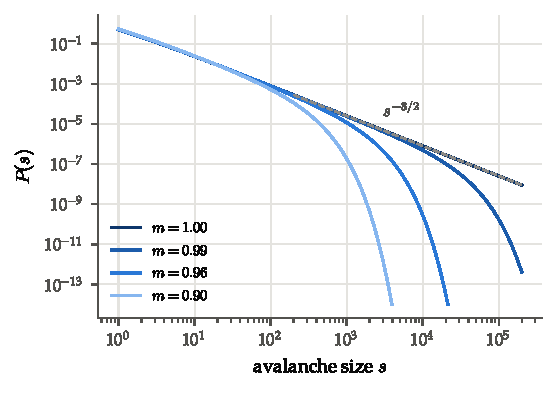
\includegraphics[width=0.55\linewidth]{theory/branching.pdf}
  \caption{Size distribution of the binary branching process for four values of the branching ratio $m$, from the exact result with the Catalan numbers
  \cref{eq:catalan}. Dashed: the critical power law $\sqrt{2/\pi}\,s^{-3/2}$.}
  \label{fig:branching}
\end{figure}

\subsection{Application to the sandpile limit}

In the fixed-drop sandpile of Chapter~\ref{ch:mapping}, a toppling sheds the force $\Delta f$, of which a fraction $1-\epsilon$, with
$\epsilon = 1/(2\ell^2+1)$, goes to the two neighbours. To turn this into a branching ratio we make the mean-field assumption that the forces of the
sites are spread uniformly over the interval of width $\Delta f$ below the threshold. A site that receives a force $\delta$ then topples with
probability $\delta/\Delta f$, and the expected number of topplings caused by one toppling is
\begin{equation}
  m = \frac{(1-\epsilon)\,\Delta f}{\Delta f} = 1-\epsilon = \frac{2\ell^2}{2\ell^2+1}.
\end{equation}
The sandpile limit is therefore a \emph{subcritical} branching process, below the critical point by exactly the bulk dissipation. The mean-field
predictions follow from \cref{eq:bp-mean,eq:bp-cutoff}:
\begin{equation}
  \avg{s} = \frac1\epsilon = 2\ell^2+1,\qquad s_c = \frac{2}{\epsilon^2}\approx 8\ell^4,
  \qquad P(s)\propto s^{-3/2}\ \text{for}\ s\ll s_c .
  \label{eq:bp-sandpile}
\end{equation}
For $\ell=6$ this predicts a power law with $\tau = 3/2$ over about four decades, up to $s_c\approx10^4$ topplings.

To test this we use the sandpile with random thresholds (noise width $w = 0.2$) of Chapter~\ref{ch:mapping}; without noise the sandpile is periodic
and has no meaningful statistics. The measured mean sizes are $\avg{s}/\ell^2 = \thsandSsix$ for $\ell=6$ and $\thsandStwelve$ for $\ell = 12$, close to
the prediction $(2\ell^2+1)/\ell^2\approx2.0$. The mean-field theory therefore gets the mean right. It gets the \emph{shape} wrong
(\cref{fig:sandpile-scaling}, right): below the cutoff, $P(s)$ decreases with an effective exponent of only $\tau_{\text{eff}}\approx\thsandTausix$, not $3/2$, and the
cutoff lies at a few tens of $\ell^2$ rather than near $8\ell^4$: nearly ten times lower than predicted for $\ell=6$, and more than twenty times lower for $\ell = 12$. The mean is
fixed by force balance and is insensitive to how the topplings are arranged; the shape is not, and the arrangement is what the branching process gets wrong.

% ======================================================================
\section{A one-dimensional approximation: random walk with losses}
\label{sec:th-randomwalk}

The failure of mean-field theory is a consequence of the dimension. On a chain, the offspring of a toppling are its two neighbours, and the
neighbours of those are again the original site and the sites next to it. Branches meet constantly, the same sites topple many times in one
avalanche, and the avalanche stays a compact interval. The random-walk picture of \cref{sec:mean} describes this geometry better.

Follow a packet of force $\Delta f$ released by a toppling. It is passed to a neighbour, which (when it topples in turn) passes it on, and at every
step the fraction $\epsilon$ is lost into the pulling spring. In the simplest version of this picture we let the whole packet survive each step with
probability $1-\epsilon$ and choose the next site at random among the two neighbours. Then:
\begin{enumerate}
  \item The packet survives $t$ steps with probability $(1-\epsilon)^t\approx e^{-\epsilon t}$, so it makes on average $1/\epsilon$ steps. Each
    step is a toppling, so the number of topplings per avalanche is of order $1/\epsilon = 2\ell^2+1$, as in mean-field theory.
  \item A random walk of $t$ steps covers a distance of order $\sqrt t$. During its lifetime the packet therefore visits an interval of length of
    order $\epsilon^{-1/2} = \sqrt{2\ell^2+1}\approx\sqrt2\,\ell$. This is the \emph{area} $a$ of the avalanche, the number of distinct sites
    that topple.
\end{enumerate}
The only length in this picture is $\ell$, and the only number of steps is $\ell^2$. If the approximation is right, the distributions of area and
size must therefore have the scaling forms
\begin{equation}
  P(a) = \frac1\ell\,F\!\left(\frac a\ell\right),\qquad P(s) = \frac1{\ell^2}\,G\!\left(\frac s{\ell^2}\right),
  \label{eq:rw-scaling}
\end{equation}
with functions $F$ and $G$ that do not depend on $\ell$. This is a sharp test: plotted as $\ell P(a)$ against $a/\ell$ and as $\ell^2P(s)$ against $s/\ell^2$,
the data for different $\ell$ must fall on one curve.

\Cref{fig:sandpile-scaling} shows that they do. For $\ell = 6$ and $\ell = 12$ the area distributions coincide over six decades, with an exponential tail
$P(a)\propto e^{-a/(\thsandDecaysix\,\ell)}$, and the mean area is $\thsandAsix\,\ell$ and $\thsandAtwelve\,\ell$, close to the estimate $\sqrt2\,\ell$. The size
distributions coincide in the bulk, and the extreme tail extends only slightly further for $\ell=12$. The noisy sandpile limit is therefore
described by a single scale, $\ell$ in space and $\ell^2$ in number of topplings, with no power law wider than about two decades in between. This
confirms quantitatively the conclusion of Chapter~\ref{ch:mapping}: the avalanches of the sandpile limit are confined to a few stiffness lengths by the
bulk dissipation.

\begin{figure}[t]
  \centering
  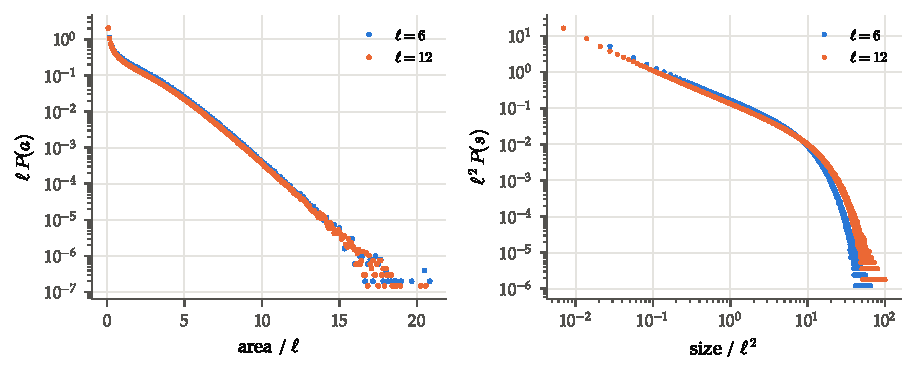
\includegraphics[width=\linewidth]{theory/sandpile_scaling.pdf}
  \caption{Scaling of the noisy sandpile limit (fixed-drop rule, $w = 0.2$) with the stiffness ratio $\ell$, as predicted by the random walk with losses
  \cref{eq:rw-scaling}. Left: number of distinct sites that topple (area). Right: number of topplings (size).}
  \label{fig:sandpile-scaling}
\end{figure}

% ======================================================================
\section{Inertial amplification in the BK model}
\label{sec:th-amplification}

\subsection{A rigid group with velocity weakening}

The sandpile is subcritical because every toppling sheds the same force, however many neighbours are also slipping. In the BK model this is not true.
\Cref{sec:one-block-event} computed the slip of a rigid group of $n$ blocks without velocity weakening; we now repeat the calculation with it.

Consider $n$ neighbouring blocks, all at threshold, that slip together by the same amount $\delta(\tau)$, while the blocks outside the group are stuck.
As in \cref{sec:one-block-event}, the spring force per block changes by $-\Omega_n^2\,\delta$ with
\begin{equation}
  \Omega_n^2 = 1+\frac{2\ell^2}{n}:
\end{equation}
the $n$ pulling springs and the two coupling springs at the ends of the group resist the motion, while the coupling springs inside the group are not
stretched. Friction is $\phi(2\alpha\dot\delta)$. With the 1991 law, $\phi(y) = (1-\sigma)/[1+y/(1-\sigma)]$, which for small velocities is
$\phi\approx(1-\sigma)-2\alpha\dot\delta$. The equation of motion per block is
\begin{equation}
  \ddot\delta = 1 - \Omega_n^2\,\delta - \phi(2\alpha\dot\delta)
  \quad\approx\quad
  \sigma - \Omega_n^2\,\delta + 2\alpha\,\dot\delta ,
  \qquad \delta(0) = \dot\delta(0) = 0 .
  \label{eq:group}
\end{equation}
This is the one-block equation of \cref{sec:one-block-event} with $\omega_1$ replaced by $\Omega_n$. The solution is therefore the same, and the slip per
block at the moment the velocity returns to zero is
\begin{equation}
  \delta_n = \frac{\sigma}{\Omega_n^2}\left(1+e^{\pi\alpha/\omega_n}\right),\qquad \omega_n = \sqrt{\Omega_n^2-\alpha^2}.
  \label{eq:group-slip}
\end{equation}

\subsection{Amplification and runaway}

\Cref{eq:group-slip} contains two sources of growth with $n$. The first is the factor $1/\Omega_n^2$: a longer group is held back by fewer coupling springs per
block. This is present without velocity weakening and gives $M_n\propto n^2$ for small groups (\cref{eq:Mn}). The second is the factor $e^{\pi\alpha/\omega_n}$:
the negative damping $2\alpha\dot\delta$ acts for the duration $\pi/\omega_n$ of the slip, and a longer group oscillates more slowly, so its slip is amplified
for longer. As $n$ grows, $\Omega_n$ decreases from $\omega_1 = \sqrt{2\ell^2+1}$ towards 1, and if $\alpha>1$ it reaches $\alpha$ at a finite group size:
\begin{equation}
  \Omega_{n^*}^2 = \alpha^2\quad\Longleftrightarrow\quad n^* = \frac{2\ell^2}{\alpha^2-1}.
  \label{eq:nstar}
\end{equation}
At $n = n^*$ the frequency $\omega_n$ vanishes and \cref{eq:group-slip} diverges. For $n>n^*$ the solutions of the linear equation \cref{eq:group} no longer
oscillate: both characteristic rates $\alpha\pm\sqrt{\alpha^2-\Omega_n^2}$ are real and positive, and the velocity grows exponentially without returning to
zero. In the linear approximation the group \emph{runs away}. In reality the slip is stopped by the nonlinearity of the friction law: as the velocity grows, friction
falls towards zero, and the group swings like an undamped oscillator about its new equilibrium. Its slip is then of order $2/\Omega_n^2$, i.e.\ of order one,
instead of order $\sigma$. We call $n^*$ the \emph{runaway size}. For $\ell = 6$ it is 9 blocks for $\alpha = 3$, 58 blocks for $\alpha=1.5$, and infinite
for $\alpha\le1$: with weak velocity weakening no group, however long, runs away.

Solving the full nonlinear equation \cref{eq:group} numerically confirms this picture. For $\ell=6$, $\alpha=3$ the slip per block is $6\times10^{-4}$ for one
block, $0.06$ at $n = n^* = 9$, and saturates at $1.5$ for very long groups: a factor of more than 2000 between a single block and a long group. For $\alpha = 1$ the
corresponding values are $3\times10^{-4}$, $0.004$ and $0.5$, and the growth is much more gradual.

\subsection{Comparison with the simulations}

A real event is not a rigid group: its blocks do not all start at threshold and do not all start at the same moment. The rigid group should therefore be read as an
upper estimate of the slip per block. \Cref{fig:amplification} compares it with the BK simulation for $\ell = 6$, $\alpha = 3$: for every event we compute the slip
per block, $M/n$, where $n$ is the number of blocks that slipped, and plot its median for each $n$. From $n = 1$ to $n = 8$ the slip per block grows by a factor
$\thampBK$ in the BK model and by $\thampRigid$ for the rigid group. The amplification is real and large, though weaker than for the idealised rigid group.

The sandpile limit behaves differently. Without noise every toppling is a slip of $\Delta f/(2\ell^2+1)$, so the slip per block equals the one-block value for every
event (dotted line). With noise a site can topple several times in one avalanche, and the slip per block grows by a factor $\thampSand$ from $n = 1$ to 8, but only because
of these repeated topplings; it never approaches the BK values. This is the missing ingredient identified in Chapter~\ref{ch:mapping}, now made quantitative: in the BK model
the force a slipping region passes to its surroundings grows with its size, so in the language of \cref{sec:th-branching} the effective branching ratio of an event
\emph{increases} as the event grows, from the subcritical value $1-\epsilon$ for a single block to a supercritical value once the slipping region exceeds $n^*$.

\begin{figure}[t]
  \centering
  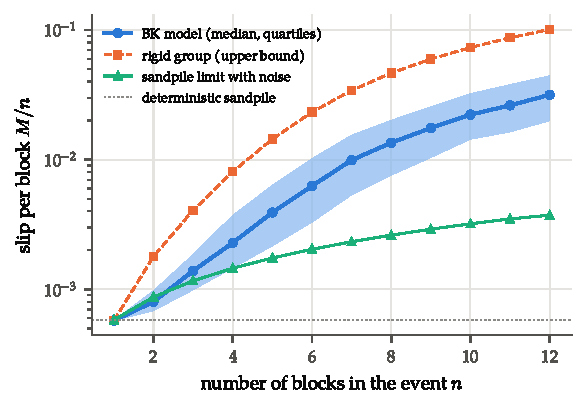
\includegraphics[width=0.62\linewidth]{theory/amplification.pdf}
  \caption{Slip per block as a function of the number of blocks in the event ($\ell=6$, $\alpha=3$, $\sigma=0.01$). BK model: median and quartiles over all events
  with $n$ blocks. Rigid group: numerical solution of \cref{eq:group}. Sandpile: fixed-drop rule with $\Delta f$ from \cref{eq:map-drop}, with noise $w = 0.2$ and
  without noise.}
  \label{fig:amplification}
\end{figure}

% ======================================================================
\section{When are there great events?}
\label{sec:th-bimodal}

\subsection{A criterion}

The size distributions of the BK model have a separate peak of great (delocalized) events for $\alpha = 3$, but not for $\alpha = 1$
(\cref{fig:alpha-test}). The runaway size suggests why. An event that is still localized can turn into a great event only if its slipping region becomes longer than
$n^*$; below that size every slip is stopped by the springs. The localization length $\tilde\xi$ of Carlson \emph{et al.} (\cref{eq:xi-tilde}) is the size of the largest
triggering zone that a growing pulse can cross without breaking out. Combining the two:
\begin{itemize}
  \item if $n^*<\tilde\xi$, localized events reach the runaway size before they reach the end of their zone, and some of them run away: there is a separate population of
    great events;
  \item if $n^*>\tilde\xi$, localized events die out before they become long enough to run away, events grow gradually, and the distribution has no separate peak;
  \item for $\alpha\le1$, $n^* = \infty$ and there are no great events in this sense for any $\ell$.
\end{itemize}
The criterion $n^*<\tilde\xi$ involves both parameters. With $n^* = 2\ell^2/(\alpha^2-1)$ and $\tilde\xi = (2\ell/\alpha)\ln(4\ell^2/\sigma)$, the ratio
\begin{equation}
  \frac{n^*}{\tilde\xi} = \frac{\alpha\,\ell}{(\alpha^2-1)\ln(4\ell^2/\sigma)}
  \label{eq:bimodal}
\end{equation}
grows with $\ell$. At fixed $\alpha$, a stiffer chain therefore needs stronger velocity weakening to produce great events. This is a prediction that a criterion based on
$\alpha$ alone would not make.

\subsection{Measuring bimodality}

To test the criterion we need a measure of how strongly the great events are separated from the localized ones. We use the \emph{depth of the minimum}: the difference
between $\ln\mathcal D(\mu)$ at the peak of the great events and at the minimum to its left (both after averaging over bins of width 0.5 in $\mu$). A positive depth means
the distribution falls, reaches a minimum and rises again; a depth of zero or below means it decreases monotonically. This depth also grows with the width of the
localized power law, so it measures the existence of a separate population, not its strength in a way that can be compared between different values of $\ell$.

We ran the BK model for ten values of $\alpha$ between 1 and 5 at $\ell = 6$ ($N = 4096$, 500 units of plate displacement each), and for $\alpha = 1.25$, 1.5, 1.75
and 2 at $\ell=12$ ($N = 8192$, 300 units). Together with the runs of Chapters~\ref{ch:mapping} and~\ref{ch:results} at $\alpha = 1$ and $\alpha = 3$, these cover
values of $n^*/\tilde\xi$ from about 0.1 to infinity.

\subsection{Results}

\Cref{fig:alpha-scan} shows the distributions at $\ell = 6$. The change with $\alpha$ is gradual for small events and abrupt for large ones. For $\alpha = 1$ and $1.25$ the
distribution of moments decreases monotonically up to the cutoff, and the distribution of the number of blocks per event is a single smooth curve. From $\alpha = 1.35$ on, a
minimum appears near $M\approx\xi$ and a separate peak of great events at $M\approx30\,\xi$, and in the distribution of blocks a plateau of events with several hundred blocks
separates from the rest. For $\alpha\ge2.5$ the shape hardly changes any more.

\begin{figure}[t]
  \centering
  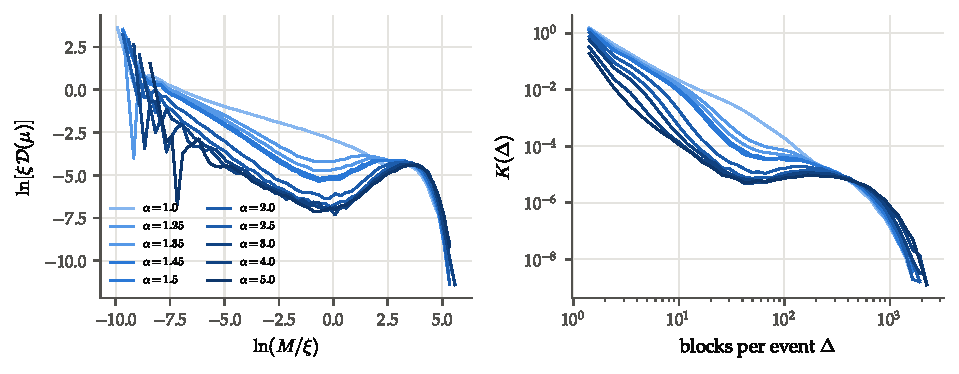
\includegraphics[width=\linewidth]{theory/alpha_scan.pdf}
  \caption{The BK model for $\alpha$ from 1 to 5 ($\ell=6$, $\sigma=0.01$, $N=4096$). Left: frequency per unit magnitude. Right: frequency of events with $\Delta$
  blocks, per unit length and unit plate displacement.}
  \label{fig:alpha-scan}
\end{figure}

\Cref{tab:bimodal} and the middle panel of \cref{fig:crossover} compare the depth of the minimum with the criterion. At $\ell = 6$ the agreement is good: the criterion
$n^* = \tilde\xi$ predicts the onset of great events at $\alpha = \thonsetsix$, and the simulations show no minimum at $\alpha = 1.25$ ($n^*/\tilde\xi = 1.39$) and a clear one from
$\alpha = 1.35$ ($n^*/\tilde\xi = 1.03$) on. Its depth then grows steadily and saturates for $\alpha\gtrsim2.5$.

At $\ell = 12$, however, the criterion fails. It predicts that the onset moves to $\alpha = \thonsettwelve$, because $n^*$ grows as $\ell^2$ while $\tilde\xi$ grows only as
$\ell\ln\ell$. The simulations show the opposite: at $\ell = 12$ a minimum is already present at $\alpha = 1.5$ ($n^*/\tilde\xi = 1.31$), with the same depth as at $\ell = 6$, and a
shallow one even at $\alpha = 1.25$ ($n^*/\tilde\xi = 2.43$). At fixed $\alpha$ the minimum is at least as deep for $\ell=12$ as for $\ell = 6$, and for $\alpha = 3$ it deepens steadily
from $\ell = 6$ to $\ell = 24$, where the criterion predicts that it should become shallower. The onset of great events therefore moves to \emph{smaller} $\alpha$ as $\ell$ grows,
not to larger $\alpha$.

The test thus refutes the criterion $n^*<\tilde\xi$ as a description of the dependence on $\ell$; its success at $\ell = 6$ is a coincidence of the numerical prefactors. What
survives is the weaker statement that great events require $\alpha>1$. The runs with $\alpha = 1$ ($\ell = 6$, 10 and 14), for which no finite group runs away, show no minimum or
only a trace of one (depth $\le0.1$), and the onset at finite $\ell$ lies somewhat above $\alpha = 1$ and approaches it as $\ell$ grows. This is consistent with the runaway of a
long group, $\Omega_\infty = 1<\alpha$, being the mechanism of the great events, but it shows that the size at which an event runs away is not $n^*$ of the rigid-group
calculation. A real event is not rigid: its slipping region is a pair of pulses that move outward, and the coupling springs inside it are stretched, so the restoring force per
block is not $\Omega_n^2$. A better estimate of the runaway size would have to start from the pulse solution of \cref{sec:bk-pulses} rather than from a rigid group.

\begin{table}[t]
\centering
\caption{Runaway size $n^*$ (\cref{eq:nstar}), localization length $\tilde\xi$ (\cref{eq:xi-tilde}) and depth of the minimum of $\mathcal D(\mu)$ for all runs with
$\sigma=0.01$. A depth of zero or below means that there is no separate population of great events.}
\label{tab:bimodal}
\begin{tabular}{cccccc}
\toprule
$\ell$ & $\alpha$ & $n^*$ & $\tilde\xi/a$ & $n^*/\tilde\xi$ & depth \\
\midrule
\tabinput{figures/theory/dip_table.tex}
\bottomrule
\end{tabular}
\end{table}

% ======================================================================
\section{The crossover moment}
\label{sec:th-crossover}

Carlson \emph{et al.} estimate that the localized events end at the crossover moment $\tilde M = 2\xi/\alpha$ (\cref{eq:M-tilde}): proportional to the stiffness
length $\xi$, inversely proportional to $\alpha$, and independent of $\sigma$. Chapter~\ref{ch:results} confirmed the independence of $\sigma$. To test the other two
dependences we need a definition of the crossover that can be applied to every run. We use the moment $M_c$ at which the effective exponent of $P(M)$, measured in
windows $[M,10M]$, first falls below 1. Since $\mathcal D(\mu) = M\,P(M)$, an effective exponent of 1 means that $\mathcal D(\mu)$ is locally flat, so $M_c$ is the
point where $\mathcal D(\mu)$ stops decreasing; it coincides with the minimum of $\mathcal D(\mu)$ when there is one, and it remains defined when there is not.

\Cref{fig:crossover} (left) shows $M_c$ for the $\alpha$-scan at $\ell=6$. For all $\alpha$ between 1.25 and 5, $M_c$ lies between $\thMcMin\,\xi$ and $\thMcMax\,\xi$, without a
trend; the prediction $2\xi/\alpha$ decreases by a factor of four over the same range. The right panel shows $M_c$ for $\alpha = 3$ and $\ell$ from 6 to 24. The prediction
$\tilde M/\xi = 2/3$ is independent of $\ell$; the measured ratio falls from $\thMcXiLsix$ at $\ell = 6$ to $\thMcXiLtwentyfour$ at $\ell = 24$, because $M_c$ itself stays between
$\thMcLmin\,a$ and $\thMcLmax\,a$ while $\xi$ grows by a factor of four. The direct positions of the minimum of $\mathcal D(\mu)$ tell the same story: they lie at
$M\approx3.5$--$6\,a$ for all five values of $\ell$.

Neither dependence of $\tilde M$ is therefore confirmed. Within the parameter range studied ($\ell\le24$), the crossover from localized to delocalized events happens at a
moment of a few units of $a$, nearly independent of $\alpha$, $\sigma$ and $\ell$. The estimate $\tilde M = 2\xi/\alpha$ has the right order of magnitude for $\ell = 6$, which
is the case Carlson \emph{et al.} studied most, but not the right scaling. It is based on the linear pulse equation, which describes a single pulse growing in a uniform
region at threshold; the crossover in the simulations is instead set by events that start in the rough configurations left by earlier events, which that calculation does
not describe. We have not found an approximate theory for the position of the crossover, and we leave it as an open question.

\begin{figure}[t]
  \centering
  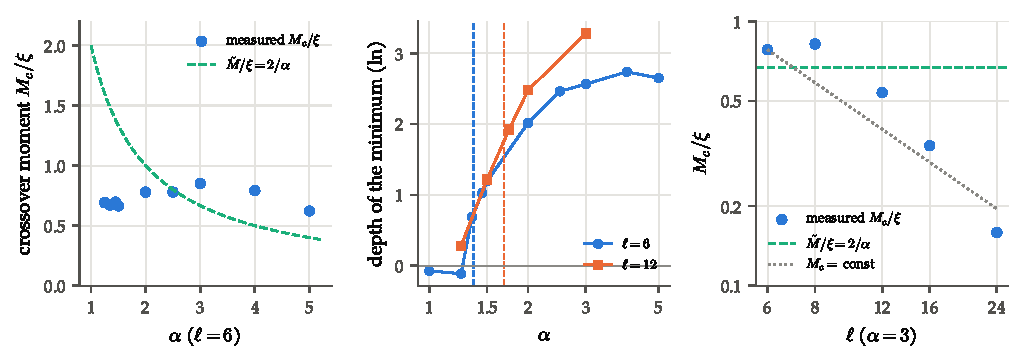
\includegraphics[width=\linewidth]{theory/crossover.pdf}
  \caption{Tests of the approximate theory. Left: crossover moment against $\alpha$ ($\ell=6$), with the prediction $\tilde M = 2\xi/\alpha$. Middle: depth of the minimum of
  $\mathcal D(\mu)$ against the ratio of the runaway size and the localization length, \cref{eq:bimodal}; runs with $\alpha\le1$ ($n^*=\infty$) are plotted at the right
  edge. Right: crossover moment against $\ell$ ($\alpha=3$), with the prediction and the line of constant $M_c$.}
  \label{fig:crossover}
\end{figure}

% ======================================================================
\section{The exponent of the localized events}
\label{sec:th-exponent}

The last question is whether any of these approximations predicts the exponent of the localized power law. \Cref{tab:alpha} gives the exponent from
maximum-likelihood fits between $\max(10M_1, 10^{-4}\xi)$ and $10^{-2}\xi$ for the $\alpha$-scan at $\ell = 6$. It is not a constant: $\tau$ rises from about 1.5 at
$\alpha=1$ to a maximum of about 1.97 at $\alpha = 3$ and decreases again for larger $\alpha$.

\begin{table}[t]
\centering
\caption{The $\alpha$-scan at $\ell=6$: exponent $\tau$ of the localized region, crossover moment $M_c$, runaway size $n^*$ and localization length $\tilde\xi$.}
\label{tab:alpha}
\begin{tabular}{ccccc}
\toprule
$\alpha$ & $\tau$ & $M_c/\xi$ & $n^*$ & $\tilde\xi/a$ \\
\midrule
\tabinput{figures/theory/alpha_table.tex}
\bottomrule
\end{tabular}
\end{table}

Two conclusions follow. First, the localized events are not a critical branching process: mean-field theory predicts the universal value $\tau = 3/2$ at its critical point,
whereas the measured exponent depends continuously on a parameter of the friction law and lies well above $3/2$ for the values studied by Carlson \emph{et al.} The value near
$3/2$ at $\alpha=1$ should not be taken as a confirmation: at $\alpha=1$ the effective exponent drifts slowly over the whole range (Chapter~\ref{ch:mapping} found $\tau\approx1.4$
in a different window), and the branching process has no reason to apply there either. Second, an exponent that varies continuously with a model parameter is not a universal
critical exponent in the sense of \cref{sec:critical}. Such non-universal exponents are known from the OFC model, whose exponent depends on the degree of conservation, and they are
another sign that the BK model is not critical in the strict sense. In the picture of \cref{sec:bk-events}, the localized events smooth the rough configurations left by great
events, so their statistics are inherited from the roughness of these configurations, which depends on how strongly the great events amplify irregularities, i.e.\ on $\alpha$.
Turning this picture into a calculation of $\tau$ would require a theory of the roughness, which we have not attempted.

% ======================================================================
\section{Summary}
\label{sec:th-summary}

\begin{enumerate}
  \item \textbf{Mean field.} The branching process gives $\tau=3/2$ at its critical point, a cutoff $s_c\propto(1-m)^{-2}$ and a mean size $(1-m)^{-1}$. The sandpile limit of the BK
    model is a subcritical branching process with $m = 1-\epsilon = 2\ell^2/(2\ell^2+1)$. Mean-field theory predicts its mean avalanche size correctly, but not the shape of the
    distribution.
  \item \textbf{Random walk with losses.} In one dimension the appropriate approximation is a random walk that loses the fraction $\epsilon$ at each step. It predicts that the noisy
    sandpile limit has a single scale, $\ell$ in space and $\ell^2$ in number of topplings, and the simulations collapse accordingly. The sandpile limit is not critical for any $\ell$.
  \item \textbf{Amplification.} A rigid group of $n$ blocks with velocity weakening slips by an amount that grows rapidly with $n$ and runs away above $n^* = 2\ell^2/(\alpha^2-1)$.
    The simulations show this amplification, weaker than for the rigid group, and the sandpile limit lacks it. This makes quantitative the failure of the mapping found in
    Chapter~\ref{ch:mapping}.
  \item \textbf{Great events.} A separate population of great events exists only for $\alpha>1$, as the runaway of long groups requires. The criterion $n^*<\tilde\xi$, which
    combines the rigid-group runaway size with the localization length, predicts the onset correctly at $\ell = 6$ ($\alpha\approx1.3$) but fails at $\ell = 12$: the onset moves to
    smaller $\alpha$ as $\ell$ grows, not to larger.
  \item \textbf{Crossover and exponent.} The crossover moment is not described by $\tilde M = 2\xi/\alpha$: it stays at a few units of $a$ for all $\alpha$ and $\ell$ studied. The exponent
    of the localized region varies with $\alpha$ and is not the mean-field value. Neither is explained by the approximations of this chapter.
\end{enumerate}

\chapter{Conclusions}
\label{ch:conclusions}

This thesis set out to answer one question: can the statistics of the one-dimensional Burridge--Knopoff model of an earthquake fault be
understood by mapping it onto a sandpile model, and can its exponents be obtained from the theory of self-organized criticality? This chapter
collects the answers, in the order of the aims listed in Chapter~\ref{ch:intro}, and lists the questions that remain open.

\section{Results}

\paragraph{Self-organized criticality in one dimension.} The Bak--Tang--Wiesenfeld sandpile is Abelian, which gives exact results in any
dimension: the mean number of topplings is the Green function of the toppling matrix, $\avg{s}\propto L^2$, and $D(2-\tau) = 2$. In one dimension
the model can be solved completely; its avalanche sizes are given by the closed formula $s = g(j)+g(l')-g(l)$, and their distribution is a function of
$s/L^2$ that is not a power law. The one-dimensional BTW model is therefore not critical, and whatever power laws the one-dimensional BK model produces
cannot come from the mechanism of the simplest sandpile (Chapter~\ref{ch:soc}).

\paragraph{The papers of Carlson and collaborators.} The 1989 and 1991 papers study different versions of the model: the 1989 version has a symmetric
friction law and a finite loading speed $\nu$, which sets the size of the smallest events; the 1991 version has an asymmetric law with a friction drop
$\sigma$ and $\nu\to0$. Their analytical estimates (the one-block event, slip pulses that grow exponentially at the sound speed, the localization length
$\tilde\xi$ and the crossover moment $\tilde M$) are the same in both, with $\nu$ replaced by $\sigma$. The one-block event, which underlies all of them,
is underestimated by a factor of about two for $\alpha=3$ when velocity weakening is neglected; we derived the corrected result,
$\delta U_1 = \sigma(1+e^{\pi\alpha/\omega})/\omega_1^2$ (Chapter~\ref{ch:bk}).

\paragraph{Implementation and validation.} The earlier implementation of this project contained several errors, among them a wrong Runge--Kutta stage, a coupling
constant tied to the system size, fixed instead of free ends, and event durations that were never recorded. The new programs (Python, with the time-critical loops
compiled by Numba) are validated by tests against exactly known results: the one-block event, a reference integrator, the energy balance, the sum rule, the Abelian
property and the exact one-dimensional solution of the BTW model (Chapter~\ref{ch:numerics}). With these programs, a run of the BK chain that records millions of events
takes minutes on a single processor core, so independent runs are executed in parallel rather than parallelising a single run.

\paragraph{Reproduction.} Both papers are reproduced. For the 1991 model the shape of the distributions and the exponents agree with the published values
($b = 0.91$--$0.96$ for $\alpha = 3$, against $0.92$; $b\approx0.36$--$0.40$ for $\alpha=1$, against $0.35$). The published curves lie, however, a factor of about five
below the normalisation defined in the paper, as the sum rule shows. For the 1989 model all five panels of Fig.~6 of Carlson and Langer are reproduced, with
$b = 0.89$--$0.94$ for $\alpha = 2.5$. Independent runs of the original length show that the shortest published runs could not determine $b$ better than about
$\pm0.1$; together with the event definition (space--time clusters of slip), this explains why the earlier version of this project failed to reproduce the 1989 figures
(Chapter~\ref{ch:results}).

\paragraph{The mapping.} Removing inertia from the BK equations gives a continuous sandpile on the chain with a fixed drop of force and bulk dissipation
$\epsilon = 1/(2\ell^2+1)$, or, with a different toppling rule, the one-dimensional Olami--Feder--Christensen model. The mapping is exact for the elementary process
(the one-block event) and for the force bookkeeping and the sum rule. It fails for everything else: the deterministic sandpile limit is exactly periodic or synchronised,
it is not chaotic, its avalanches are confined to a few stiffness lengths, and the friction parameters only set the unit of slip. Adding random thresholds removes the
periodicity but not the confinement. None of the features of the BK size distribution beyond the smallest events survives (Chapter~\ref{ch:mapping}).

\paragraph{Is the BK model critical?} Not in the strict sense of self-organized criticality. Its localized events follow a power law over a window bounded below by the
microscopic events and above by a crossover at a moment of a few units of $a$, and the great events form a separate population with a peak and a sharp cutoff. The friction
drop $\sigma$, which Carlson \emph{et al.} identify as the critical parameter, changes only the smallest events. The window of localized events and the range of great events
both widen as the stiffness ratio $\ell$ grows, while the exponent drifts slowly, so the continuum limit $\ell\to\infty$ remains an open possibility for scale invariance
(Chapter~\ref{ch:results}).

\paragraph{Approximate theory.} Mean-field theory (the branching process) describes the sandpile limit as a subcritical process with branching ratio $1-\epsilon$; it
predicts the mean avalanche size but not the distribution, which is instead described by a random walk with losses and collapses with the single scale $\ell$. The BK model
differs by inertial amplification: a rigid group of $n$ blocks slips by an amount that grows rapidly with $n$ and runs away above $n^* = 2\ell^2/(\alpha^2-1)$, and the
simulations show the same amplification. Great events require $\alpha>1$, the condition for a long group to run away. A sharper criterion, $n^*<\tilde\xi$, predicts their onset
correctly for $\ell = 6$ but was refuted by new runs at $\ell = 12$, where the onset moves to smaller $\alpha$ instead of larger (Chapter~\ref{ch:theory}). The predicted crossover moment $\tilde M = 2\xi/\alpha$ is not confirmed, and the exponent of the localized events depends on $\alpha$,
which rules out a universal mean-field exponent.

\section{The answer}

The one-dimensional Burridge--Knopoff model cannot be mapped onto a sandpile model. The obstacle is not a detail of the toppling rule or the absence of disorder, but the
inertia of the blocks: with velocity-weakening friction, a slipping region gains momentum and passes on more force the larger it becomes, so that its effective branching ratio
grows with its size, while in any sandpile built on static force transfer every toppling passes on the same fraction $1-\epsilon$ of a fixed drop. This amplification produces the
great events, the chaotic dynamics and the dependence on $\alpha$; its absence makes the sandpile limit subcritical and confined to the scale $\ell$. The Gutenberg--Richter-like
statistics of the BK model are therefore intrinsically dynamical, and they are not self-organized critical in the sense of the sandpile models.

\section{Open questions}

\begin{itemize}
  \item \textbf{The crossover.} The crossover from localized to great events lies at a moment of a few units of $a$, nearly independent of $\alpha$, $\sigma$ and $\ell$ in the range
    studied. A theory of its position, and a test whether it eventually scales with $\xi$ for $\ell\gg24$, are missing.
  \item \textbf{The runaway size.} The onset of great events lies at $\alpha\approx1.3$ for $\ell=6$ and below $1.25$ for $\ell = 12$. An estimate of the size at which an
    event runs away, based on the pulse solution rather than on a rigid group, should explain this dependence on $\ell$.
  \item \textbf{The exponent of the localized events.} It depends on $\alpha$, with a maximum $\tau\approx2$ near $\alpha = 3$. In the picture of Carlson \emph{et al.} it is set by
    the roughness that great events leave behind; a quantitative theory of that roughness would be needed to predict it.
  \item \textbf{The continuum limit.} Whether the window of the localized power law becomes infinite and its exponent converges as $\ell\to\infty$ requires chains with $\ell\gtrsim100$,
    which are within reach of the present programs with longer runs.
  \item \textbf{A dynamical cellular automaton.} A sandpile-like model that carries a velocity, or a rule in which the force passed on grows with the size of the slipping region,
    might reproduce the BK statistics at a fraction of the cost. The runaway of long slipping regions for $\alpha>1$, found in Chapter~\ref{ch:theory}, is the property such a model would have to reproduce.
  \item \textbf{Two dimensions.} The OFC model was derived from a two-dimensional BK model. Whether inertia plays the same role there, and whether the two-dimensional sandpile limit
    is closer to criticality, is the natural extension of this work.
\end{itemize}


\printbibliography[heading=bibintoc]

\end{document}
